\chapter{Pressure Anisotropy Probe}
\label{sch:pa_probe}

Pressure anisotropy, as discussed in \ref{ss2:intro_PA_what}, is a difference between the average kinetic energy parallel to the magnetic field vs. perpendicular to the field. During reconnection, our interest lies in understanding the electron anisotropy as simulations show that it can have major impacts on the reconnection dynamics \cite{Ohia_Egedal_Lukin_Daughton_Le_2012}.

\section{Measurement Methods}

% We need some way of actually measuring the electron distribution function or at least the parallel and perpendicular temperatures so let's examine a number of possibilities.
We require the measurement of the temperatures parallel and perpendicular to the magnetic field to identify pressure anisotropy. There are a number of diagnostics that can attain those measurements with each being of varied complexity and requirements.

\subsection{Thomson Scattering}

Thomson scattering has long been used in the fusion plasma community for measuring electron distribution functions.

% \subsubsection{Basics}

These diagnostics use Thomson scattering where a laser scatters off electrons. By measuring the spectrum of the scattered radiation for a single direction, the distribution function in that direction can be attained. Then, if the measurement direction is changed, a new direction of the distribution function can be measured.

Thomson scattering works well as a localized measurement that's measurement volume is determined by the optics of the beam and collection.% Our system is not so reproducible that this high localization is necessary but it is nice nevertheless.
Since Thomson usually operates in a pulsed fashion, the timing and duration of pulses can be highly controlled to allow for very temporally localized measurements on the scale of nanoseconds. % Check this.

It's also non-perturbative and thus is especially useful in fusion devices where physical probes are impossible. Additionally, laser based diagnostics do not require the use of long probe shafts except for the case of moving collection optics near the measurement area.

This diagnostic faces a number of issues that would need to be addressed for application to TREX including the following:
\begin{itemize}
    \item The startup cost for the laser and hardware needed is large along with the training/learning required to get the system working.
    \item Thomson scattering is signal-to-noise limited and attaining a sufficient number of photons is difficult. Because of the size of our machine (and thus the distance from the measurement location of collection optics) and the relatively low densities, this would decrease the number of measured photons.
    \item We want to measure the evolution in time of the distribution function. Thomson scattering is often usually sampling at a maximum rate of 1 kHz. Some systems pulse the laser briefly at a higher rep rate but this is still too low of temporal frequency for our plasma dynamics.
    \item Since our system triggers at slightly different times for each shot, a scheme would need to be developed that could be triggered based on some sort of plasma dynamics or current ramp up.
    \item The low temperatures of our system (on the order of 10s of eV) necessitate the use of high spectral purity lasers or measurement optics. This raises the cost of setup and reduces the available lasers that could be used.
\end{itemize}

\subsection{Retarding Field Energy Analyzer}

A retarding field energy analyzer (RFEA) uses a set of conducting grids at different potentials to repel all particles up to some kinetic energy. They can be used for either electrons or ions but here we'll discuss electron RFEAs.

% \subsubsection{Basics}
% TODO: Is cuboid the right term.
A planar RFEA is often a small box with a hole on one side where particles enter. Particles initially pass through an aperture such that particles mostly from a single direction are measured, then ions are repelled using a grid at a high positive potential. Electrons of a minimum energy are selected via another grid at a negative potential, and finally electrons are collected and the current is measured.

% \subsubsection{Pros}

RFEAs accurately measure the high energy tail of a distribution. The electron distribution is extracted by taking the derivative of the measured current with respect to the applied voltage at a single time point by using many shots to sample the IV-characteristic. For our configuration we would use a static repelling potential because sweeping the voltage in time would not be feasible in the experiment timescales. RFEAs have been shown to work to very high sampling rates so a continuous evolution of plasma temperature could be measured \cite{Hu_Rovey_Zhao_2017}.

% \subsubsection{Cons}

Since RFEAs need multiple grids they are usually somewhat sizable (around a centimeter on all sides). In the case of creating a multidirectional probe, which would vastly accelerate data collection, the size of the probe would become large and an understanding of non-local perturbative physics may be required for data interpretation. Since our plasma potential changes drastically during a shot, a measurement of that potential would be needed for RFEA interpretation which could be done with an additional probe near the RFEA but would increase the size and complexity.

Overall, an RFEA is a promising option especially for the study of particle energization during reconnection but because of lack of experience and probe miniaturization was not chosen for TREX.

\subsection{Langmuir Probes}

Langmuir probes come in many possible configurations and are relatively easy to build (a description of these probes can be found in section \ref{sse:multitip_langmuir_what}).

% \subsubsection{Basics}

Common probe setups are the following:
\begin{itemize}
    \item A single tip cylindrical probe which is a long thin wire. This is useful for measuring the isotropic plasma IV-characteristic from which plasma parameters can be extracted either by fitting or taking the derivative of the probe current with respect to voltage (specifically for getting the electron distribution function) \cite{Godyak_Demidov_2011}.
    \item Two plates pointed in opposite directions (like that seen in fig. \ref{fig:multitip_mach_effect}) which can measure the ion drift velocity by measuring the ratio of ion currents to each plate \cite{Chung_2012}.
    \item A ball-pen probe consisting of a shield and collector. The collector is retracted inside the shield such that only a limited number of electrons can hit the probe because their gyroradii force them to instead hit the shield. By changing the retraction depth this can be used to balance the electron and ion currents such the plasma potential can be directly measured but requires high magnetic fields. % TODO: add citation.
    \item A directional probe where an alumina sheath around a cylindrical probe has a hole perpendicular to the axis of the cylinder. The hole is rotated between shots to collect at different angles relative to the plasma flow and the ion saturation current is measured. % TODO: add citation
\end{itemize}

The TREX group had a significant amount of experience designing, building, and operating Langmuir probes for studying magnetic reconnection that work well to attain accurate isotropic plasma parameters at high frequencies. These probes are relatively cheap and we already have a number of materials needed for their construction.

Utilizing Langmuir probes for directional measurements of the electron distribution has not yet been well documented although there are many setups that use direction for extracting the ion flow. One possible reason for this is that many terrestrial experiments lack the ability to generate anisotropic electron distributions in the regions accessible by a Langmuir probe. Since the theory is lacking in understanding anisotropic distributions we will need to develop our own. 

% \subsection{Solution}

Comparing all of the aforementioned solutions, we've designed a multi-tip directional Langmuir probe that leverages the expertise of our group and funding requirements.

\section{Hardware}

The pressure anisotropy probe (PA probe) uses many of the same designs as the multi-tip Langmuir probe so we focus here on highlighting significant differences.

% \subsection{Shaft Components}

% The garages, shaft materials, and usage of centering collets is the same as described in \ref{sss:multitip_shaft_components}. The only difference is the feedthrough.

% \subsubsection{Feedthrough}

\begin{figure}
    \centering
    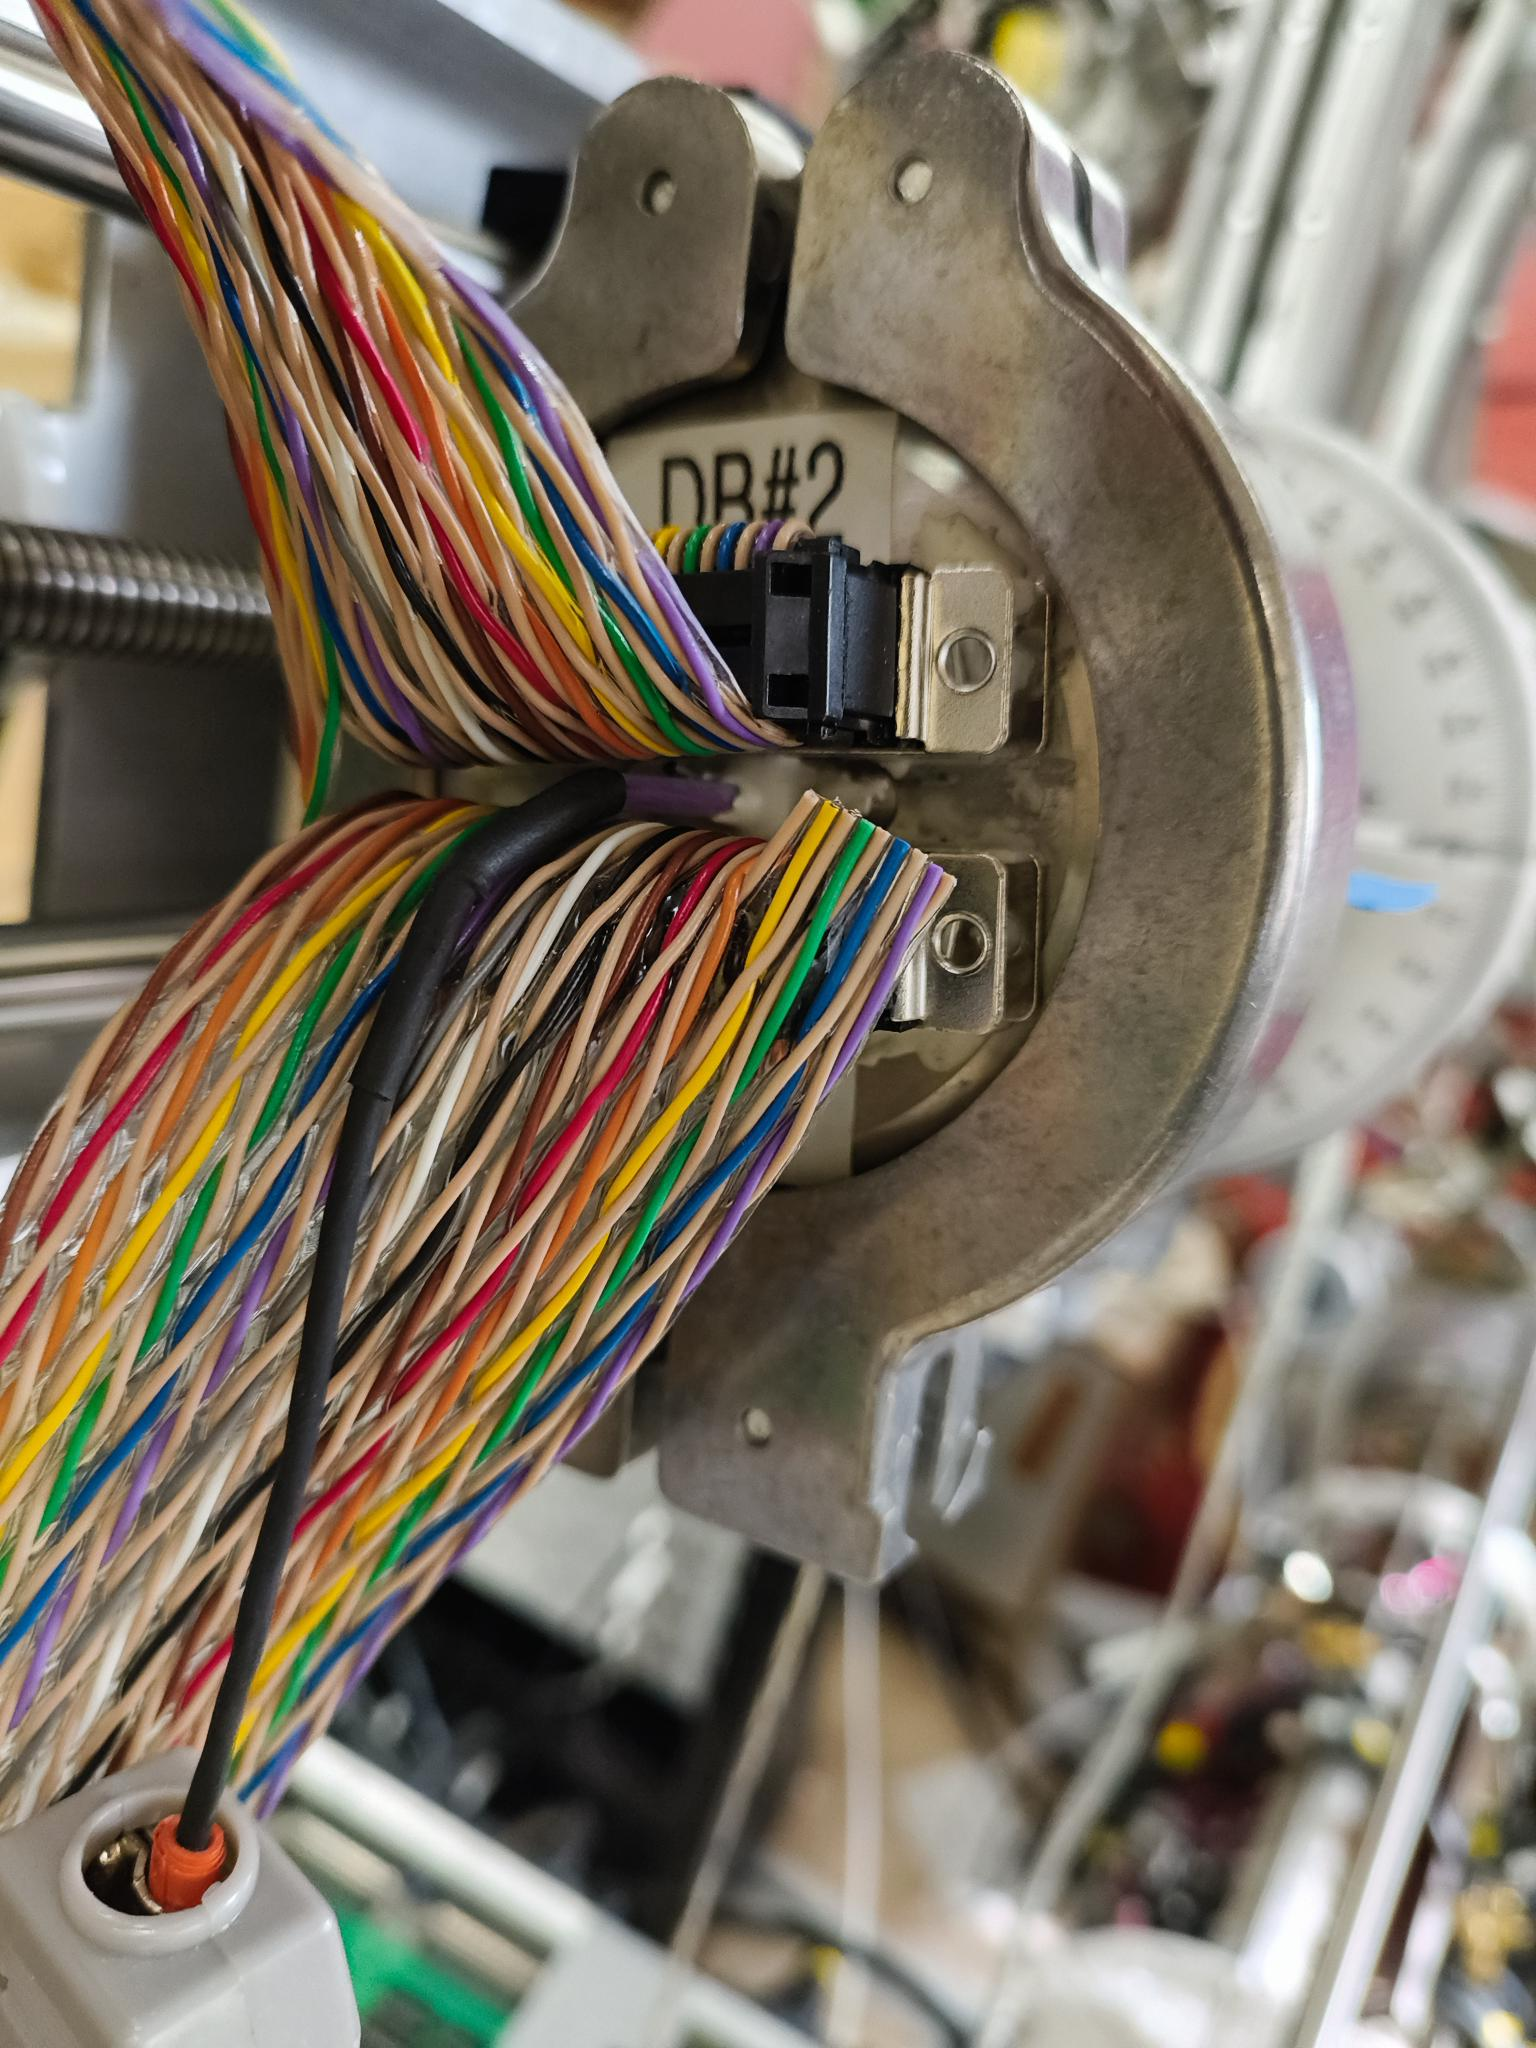
\includegraphics[width=0.5\textwidth]{chapter_pa_probe/figures/pa_feed_thru.jpeg}
    \caption{Image of the PA probe feedthrough with both DB-25s connected with ribbon cables for attaching to the probe tips. The central black tubing carries the B-dot signals from the probe to the digitizer.}
    \label{fig:pa_feedthroughs}
\end{figure}

For the feedthroughs in figure \ref{fig:pa_feedthroughs}, we use the same basic setup of two hermetically sealed DB-25s mounted to a KF-50 flange except for an addition of a through-hole that carries B-dot signals. This is made by drilling a hole through the flange and then passing twelve wires along with a structural wire through the hole. Vacuum sealing is done using an epoxy and mounting connection are soldered to both ends of the signal wires (an internal circuit board and an external DB-15) while heat shrink and teflon tubing is used to protect the signal wires.

% \subsection{Tip Components}

\begin{figure}
    \centering
    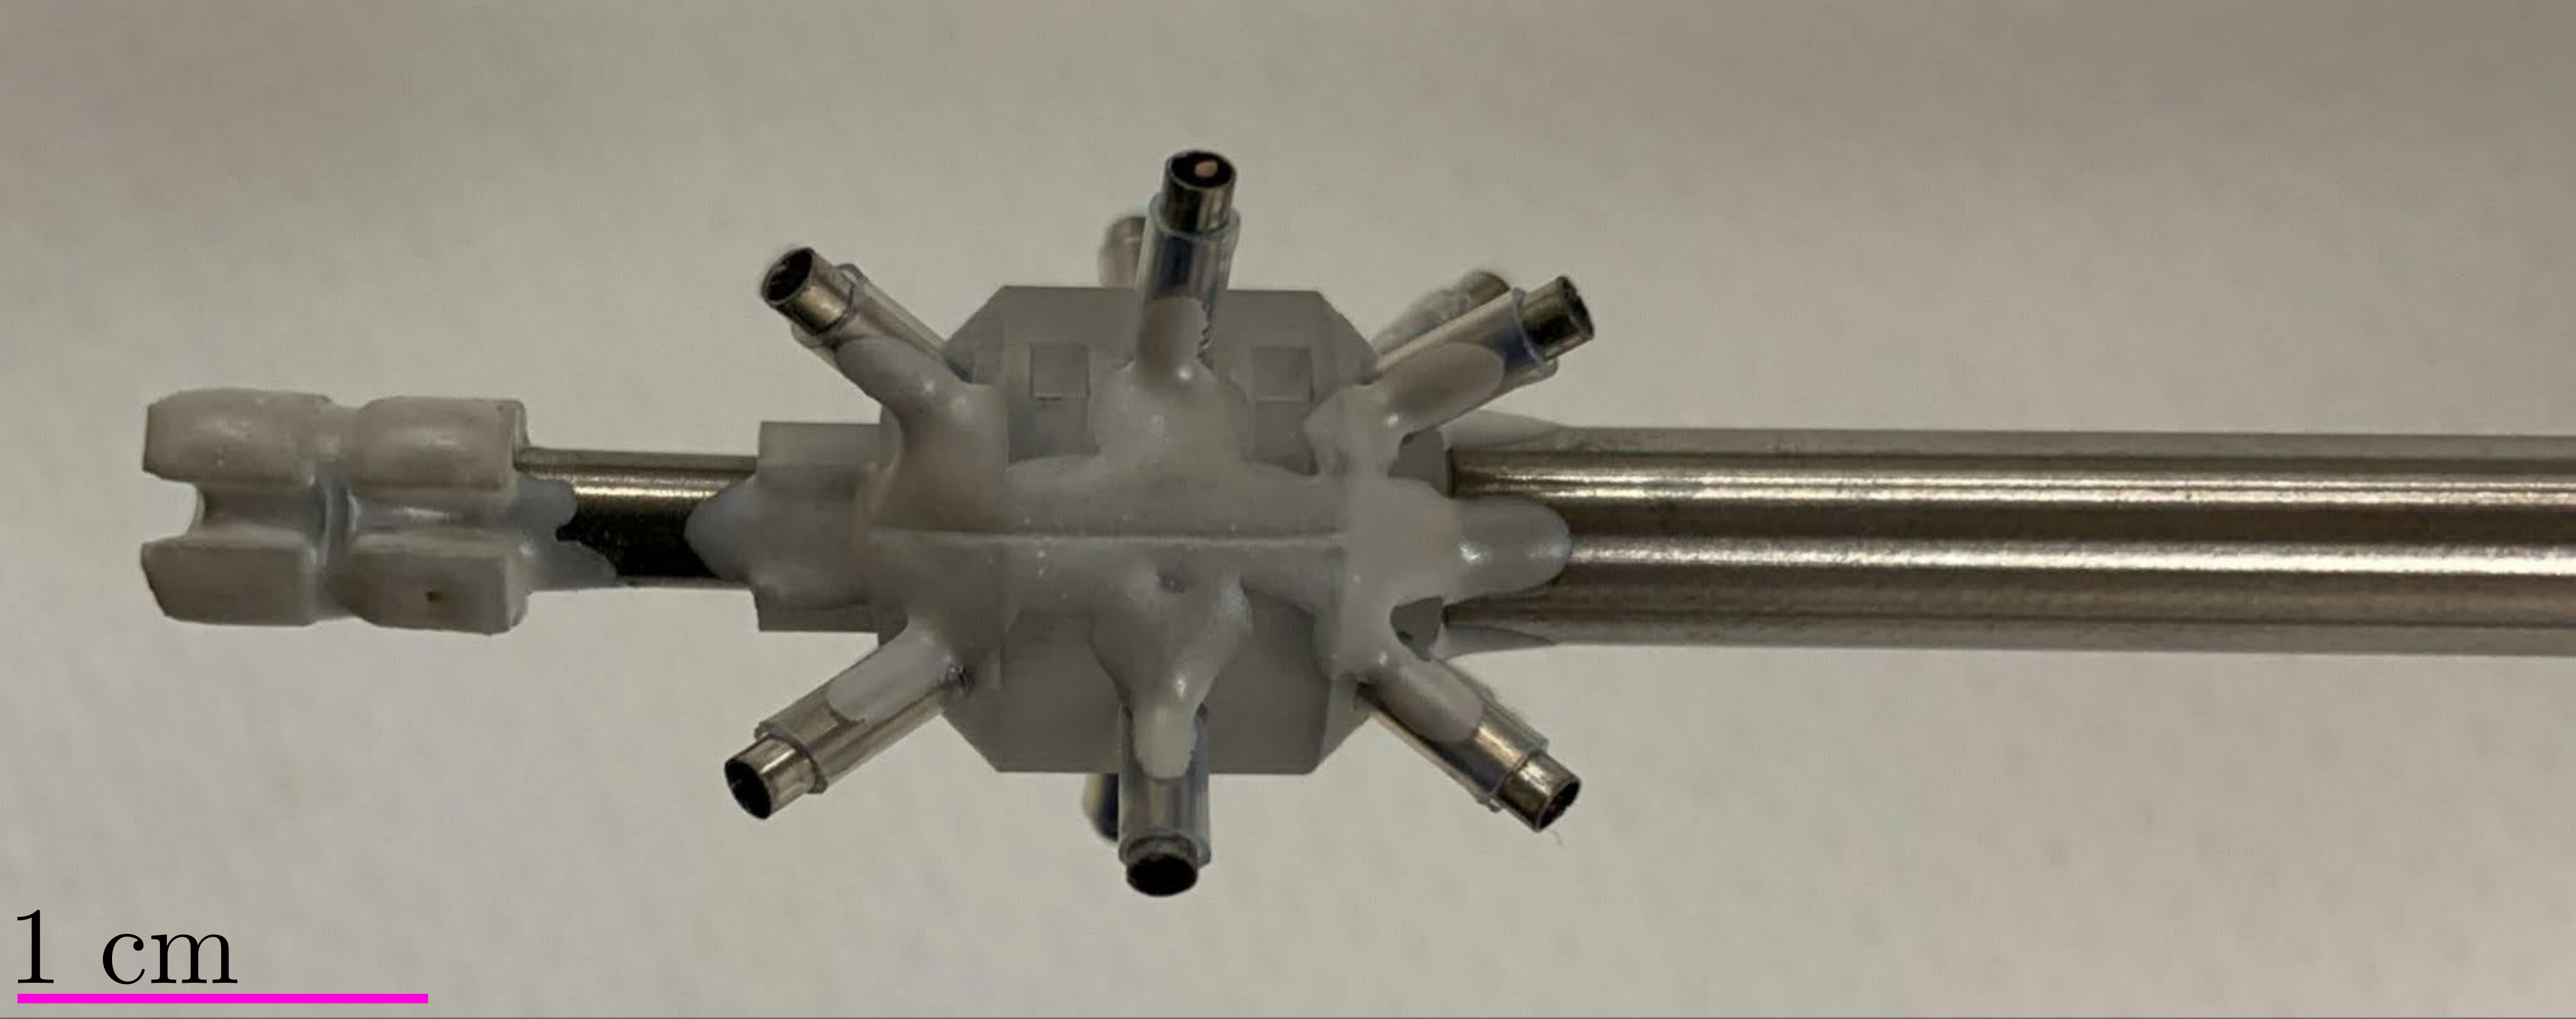
\includegraphics[width=\textwidth]{chapter_pa_probe/figures/probe_image_with_scale.png}
    \caption{Image of the end of the probe. On the far left is a 3-axis hand wound B-dot probe which is attached to the PR probe at center via a short length of stainless steel tubing. The central probe body is composed of two halves joined with epoxy. Each of the twelve tips point outwards from the center of the probe. The rightmost tubing connects the probe body to the shaft.}
    \label{fig:pa_image}
\end{figure}

\begin{figure}
    \centering
    \begin{subfigure}{.5\textwidth}
    \centering
    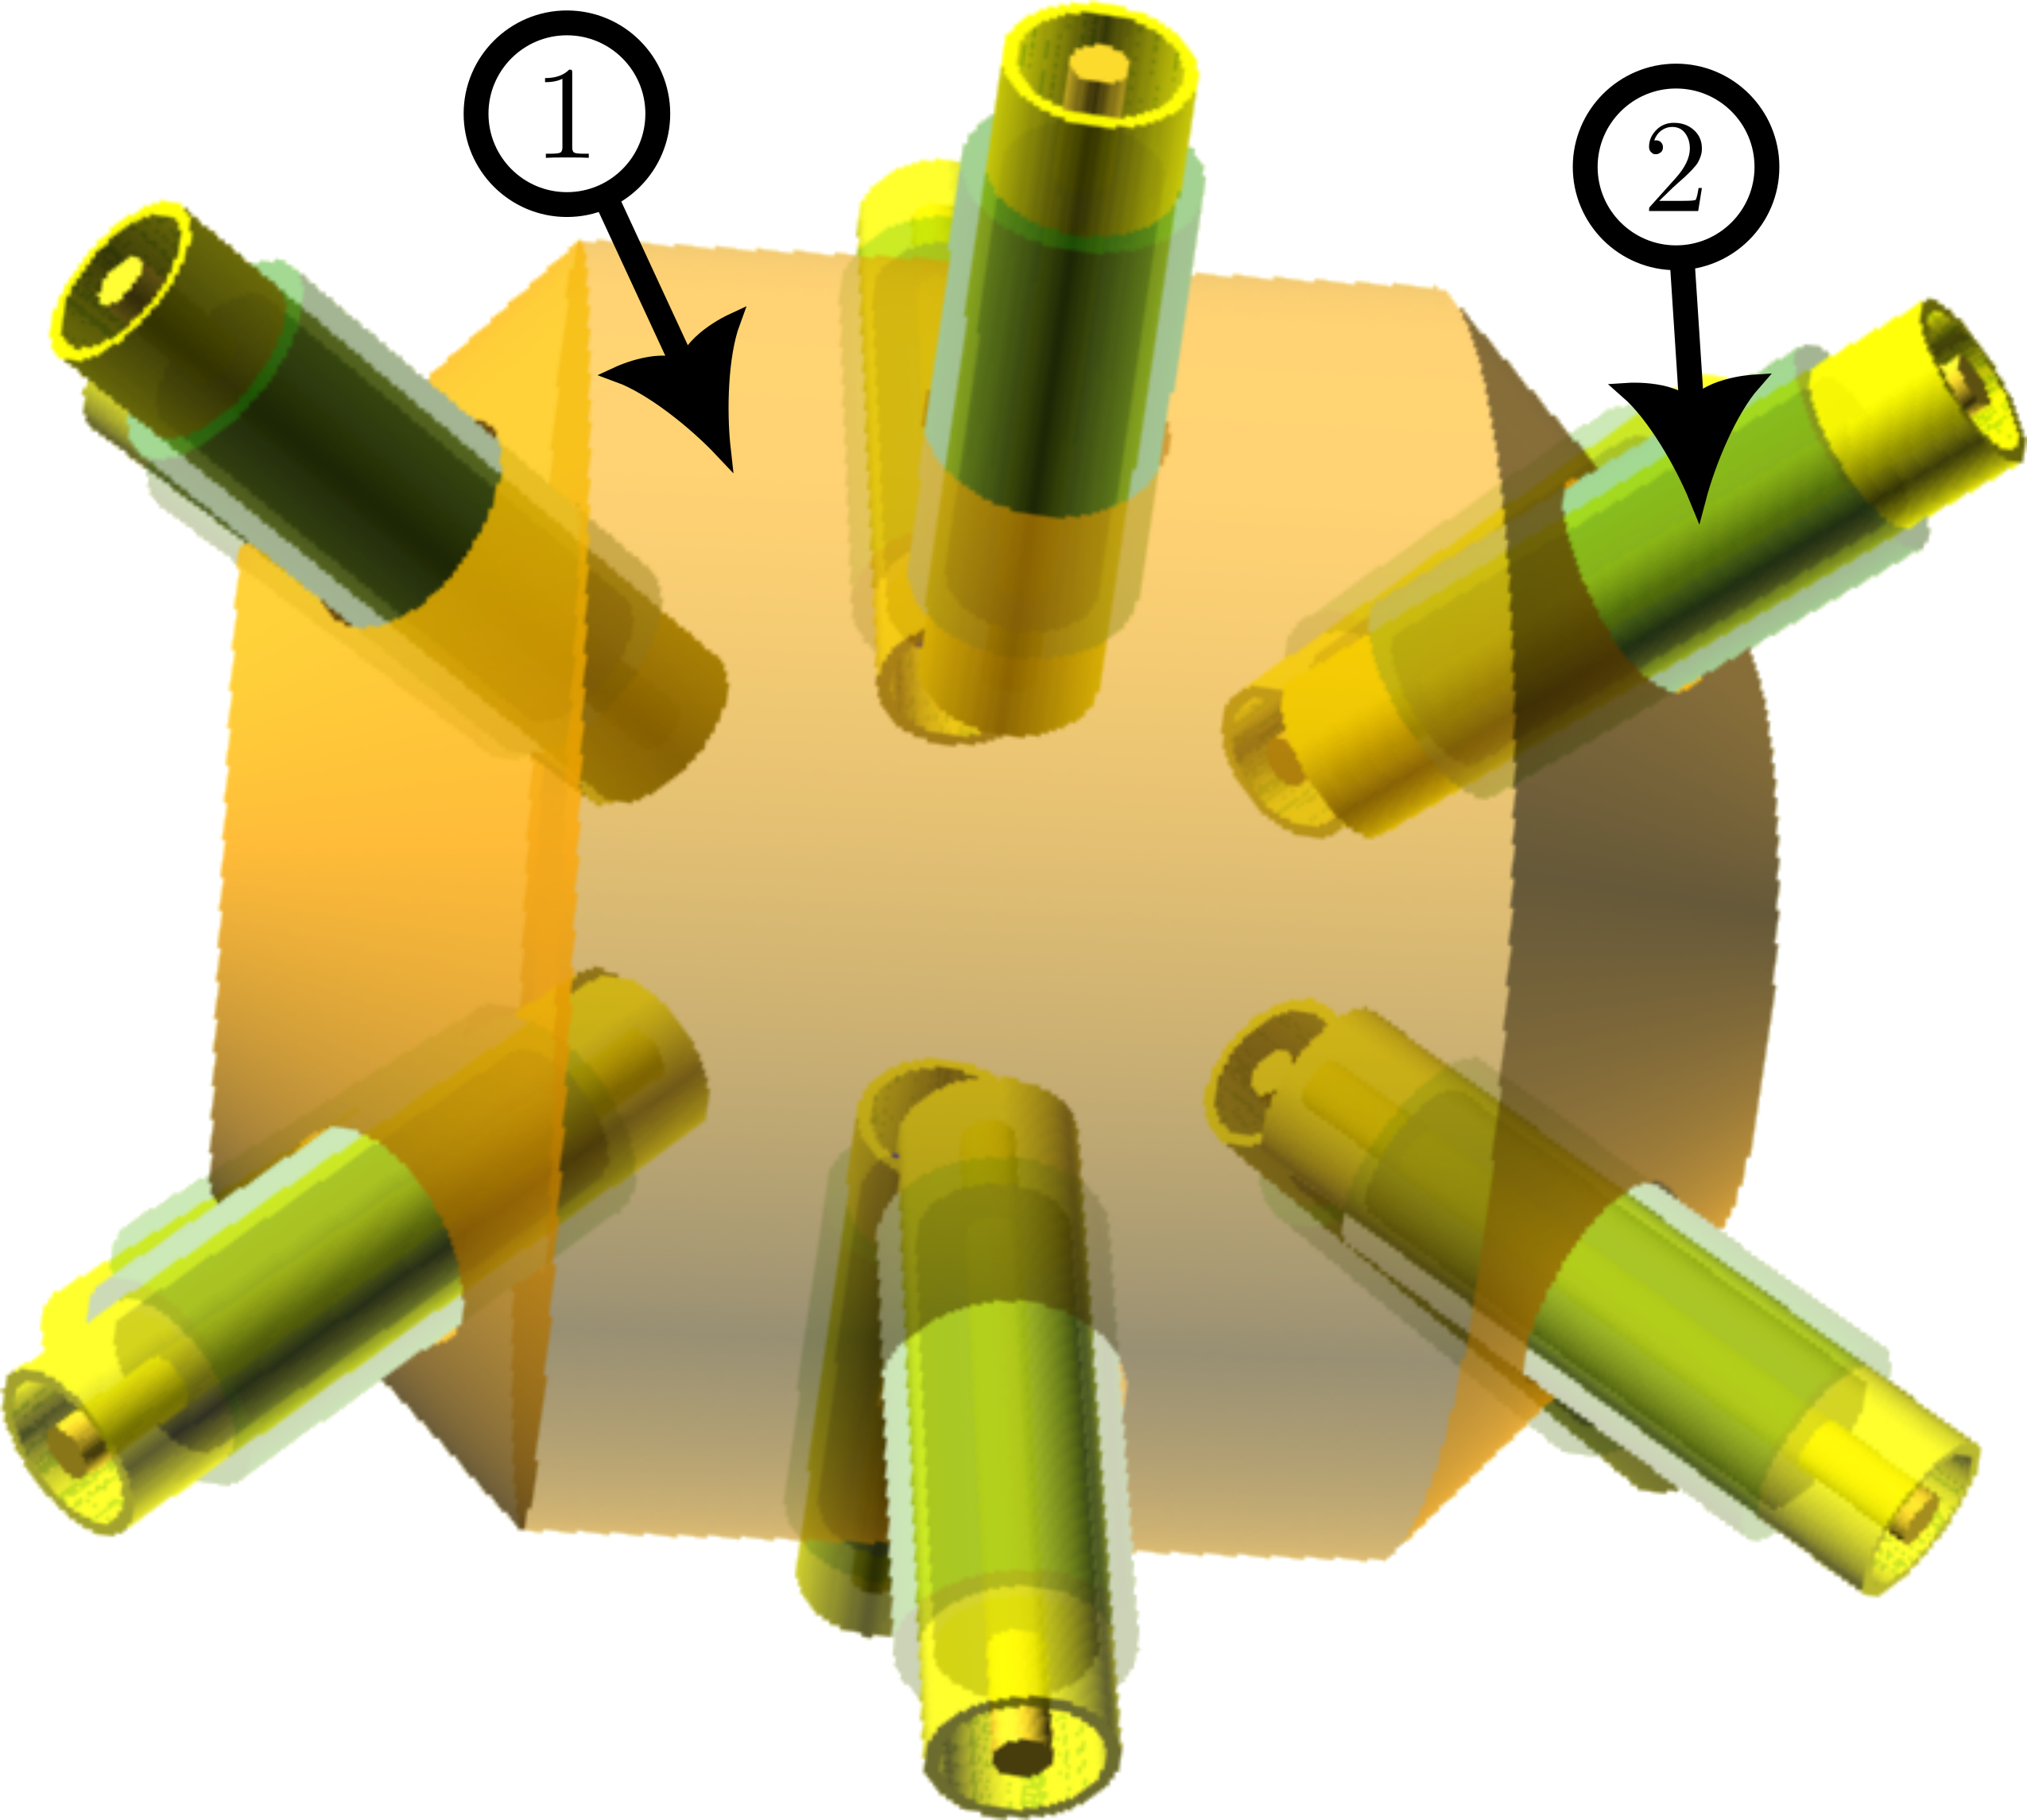
\includegraphics[scale=0.9]{chapter_pa_probe/figures/cad_body_image.png}
    \caption{Full probe}
    \label{fig:pa_full_probe_cad}
    \end{subfigure}%
    \begin{subfigure}{.5\textwidth}
    \centering
    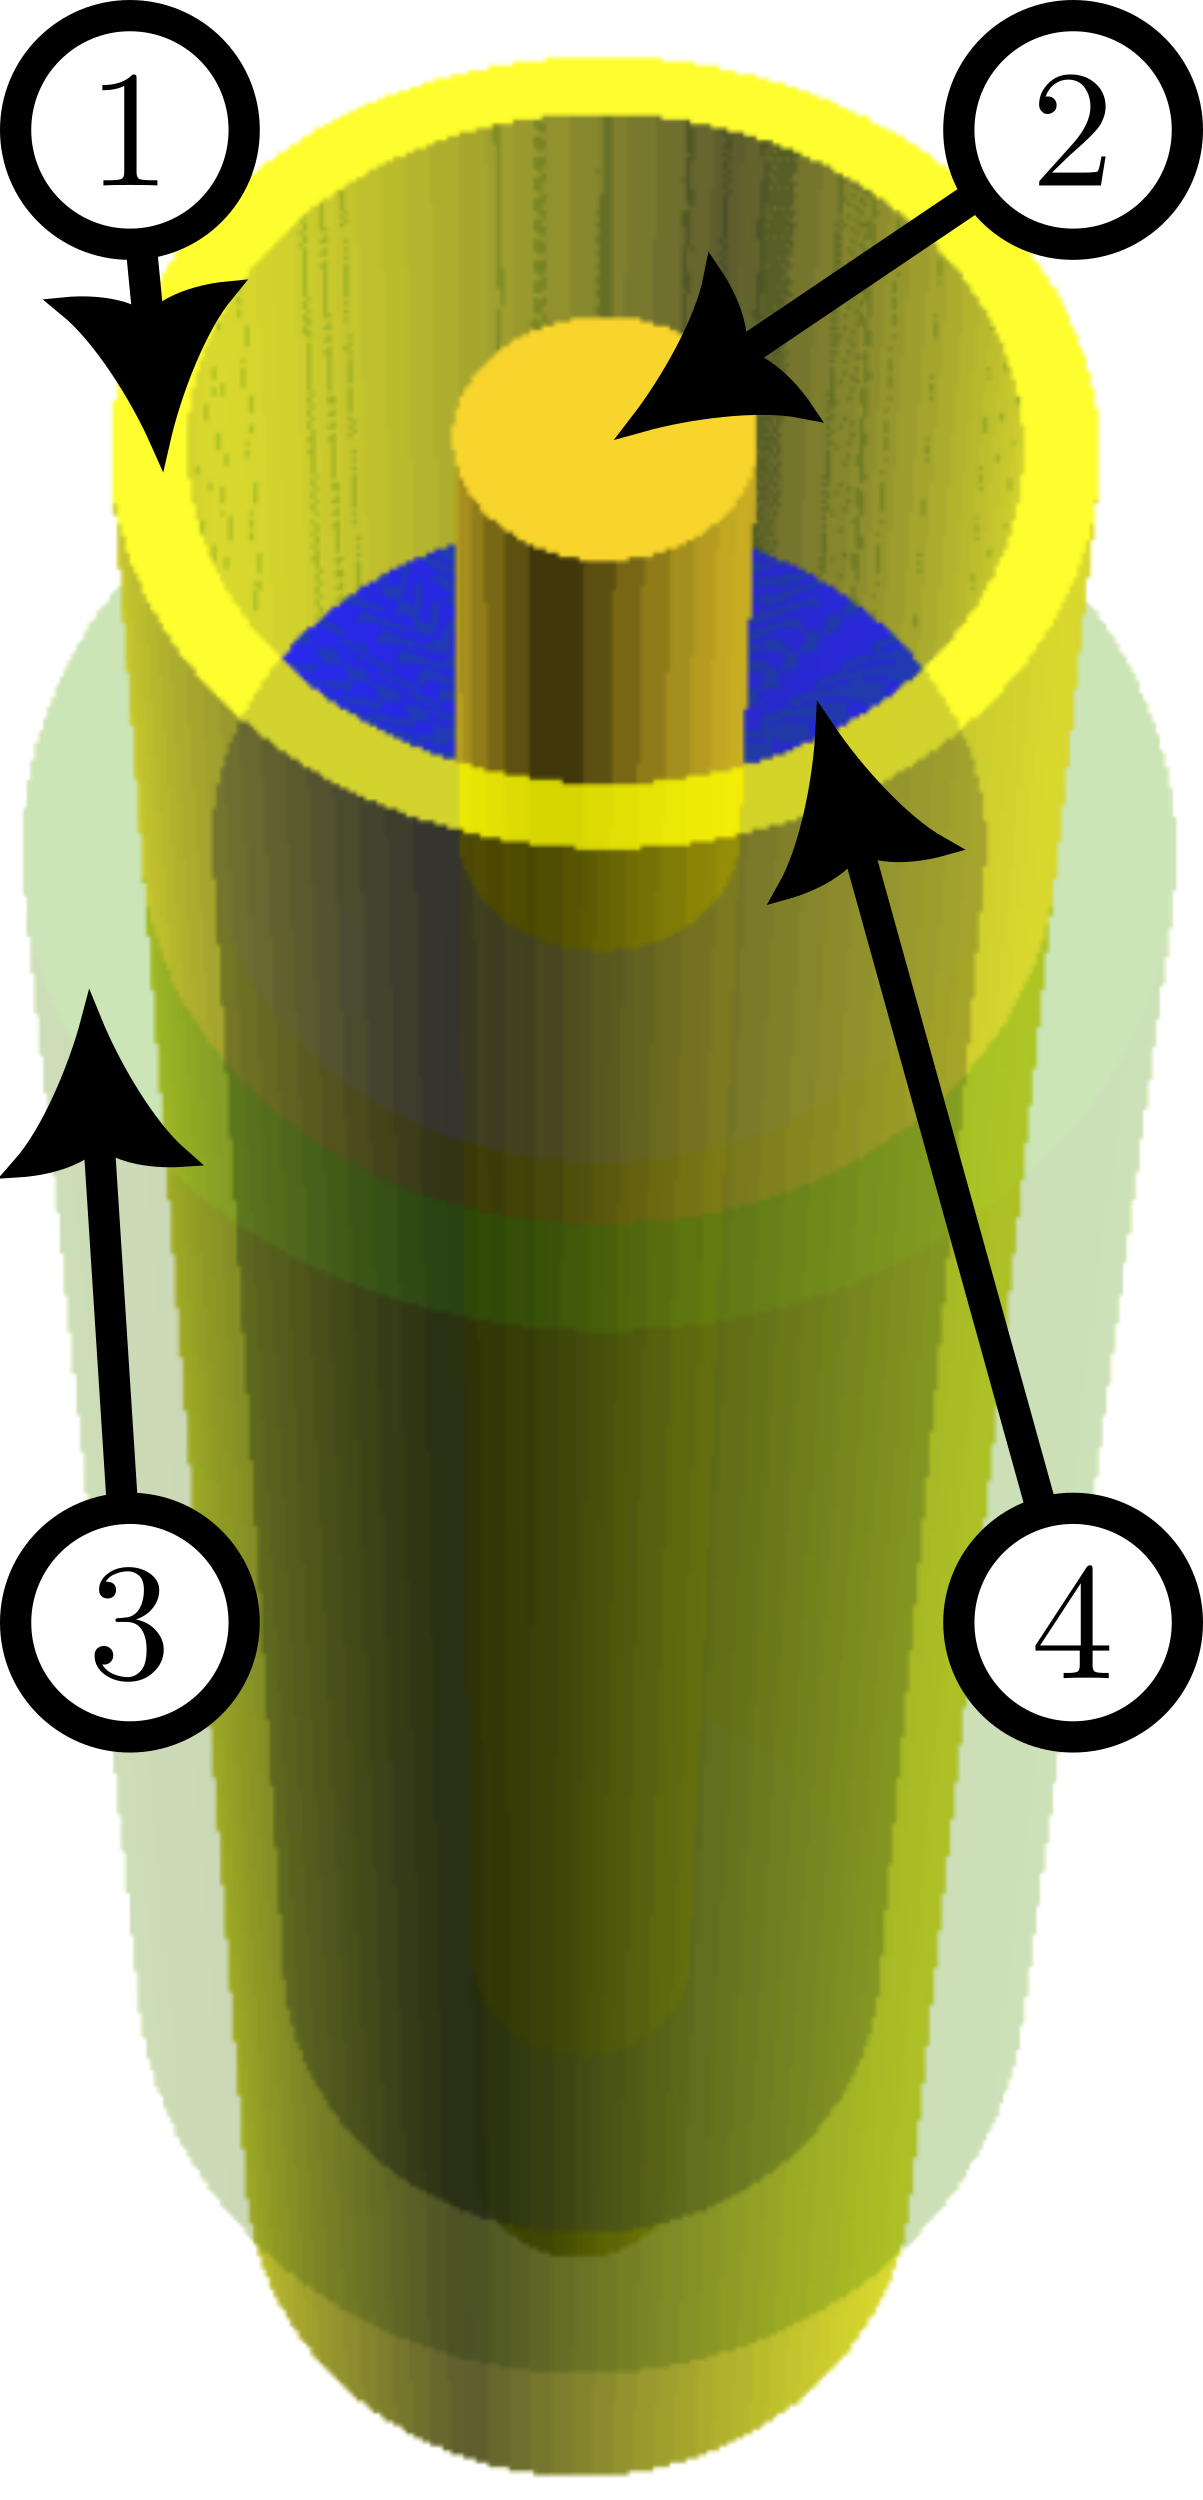
\includegraphics[scale=0.9]{chapter_pa_probe/figures/cad_tip_image.png}
    \caption{Single tip}
    \label{fig:pa_single_tip_cad}
    \end{subfigure}
    \caption{CAD diagrams of the PA probe. \ref{fig:pa_full_probe_cad} shows the 3D-printed body (1) and tips (2) of the PA probe. \ref{fig:pa_single_tip_cad} shows the shell (1) and core (2) conductors where the shield is protected by insulation (3) and the conductors are isolated from each other via more insulation (4).}
    \label{fig:pa_cad}
\end{figure}

% \paragraph{Two sides}

The probe, as can be seen in figure \ref{fig:pa_image} and \ref{fig:pa_cad}, is built in two halves of six tips each where each tip consists of stainless steel tubing, teflon outer insulation, and PTFE insulated solid core wire. Each tip is individually constructed then threaded through the probe body until finally both halves are epoxied together.

% \subsubsection{Tip material + size}

As compared to the multi-tip probe, the PA probe tips use stainless steel and copper as conductors instead of molybdenum. Although both of these metals have higher secondary electron emission coefficients they are both still small at the low temperatures our plasmas attain \cite{Dekker_1958}.

% \paragraph{Shell}

% The shell of the tip is made of 7 mm of stainless steel tubing. On one side, a wire is soldered for measuring the current to the shell and the other side is exposed to the plasma.

% \paragraph{Core}

% The core on the other hand is just 24 AWG wire that is placed inside the shell with a limited amount of wire exposed from it's PTFE insulation. The other side of the wire is also soldered for measurement.

% \subsubsection{Tip Shielding}

% To restrict current to the tip to not overwhelm measurement and reduce tip heating, we shield both the shell and the core.

% \paragraph{Shell Shielding}

% The shell is shielded using teflon tubing that exposes some of the tip on the plasma facing side and helps to move the measurement region away from the body to avoid shadowing effects (see \ref{fig:multitip_mach_effect}) as we want the shell to collect isotropically.

% \paragraph{Core Shielding}

% The core is shielded in two ways. The insulation on the core limits how much is exposed in total while the height of the core cylinder face relative to the shell edge limits the projected area the core sees as discussed in \ref{spg:pa_area}.

% \subsection{B-dot Coils}

% The design of the B-dot probe on the end of the PA probe is the same as that for the multi-tip Langmuir probe as discussed in \ref{sss:multitip_bdot}.

% \subsection{Length Scales}

% The plasma parameters we must consider are the same as those for the multi-tip probe but we have a few other probe length scales specific to the PA probe which can all be seen in table \ref{tab:pa_length_scales}.

\begin{table}
\begin{center}
\begin{tabular}{|r|c|c|c|}
    \hline
    Name & Symbol & Equation & Value \\
    \hline\hline
    Core radius & $r$ & --- & 3e-4\\
    \hline
    Shell inner radius & $r$ & --- & 7e-4\\
    \hline
    Shell outer radius & $r$ & --- & 8e-4\\
    \hline
    Exposed shell length & $l$ & --- & 4e-3\\
    \hline
    Exposed core length & $l$ & --- & 3e-3\\
    \hline
    Top of core to top of shell & $l$ & --- & ~1e-3\\
    \hline
    Poloidal angular separation & --- & --- & $45$\textdegree \\
    \hline
    Toroidal angular separation & --- & --- & $45$\textdegree \\
    \hline
    Tip-to-tip separation & --- & --- & ~1e-2\\
    \hline
    B-dot coil side length & --- & --- & 3e-3 \\
    \hline
    Debye length & $\lambda_D$ & $\sqrt{\frac{\epsilon_0 T_e}{n e}}$ & 3e-5 \\
    \hline
    Ion Gyroradius & $r_i$ & $\frac{m_i \sqrt{2 m_i \bar{v}_i}}{e B}$ & 6e-1 \\
    \hline
    Electron Gyroradius & $r_e$ & $\frac{m_e \sqrt{2 m_e \bar{v}_e}}{e B}$ & 1.5e-1 \\
    \hline
    Ion mean free path & $\lambda_i$ & $\frac{\bar{v}_i}{\nu_{i,i}}$ & 9e-4 \\
    \hline
    Electron mean free path & $\lambda_e$ & $\frac{\bar{v}_e}{\nu_{e,e}}$ & 4.5 \\
    \hline
    Electron energy relaxation length & $\lambda_\mathcal{E}$ & * Eq. 5 & 4.5 \\
    \hline
    Sheath thickness & $h$ & $\sim \lambda_D$ & 3e-5 \\
    \hline
\end{tabular}
\end{center}
\caption[*Pressure Anisotropy Probe Length Scales]{Length scales of the PA probe. All lengths are in meters and are approximate. Refer to table \ref{tab:multitip_length_scales} for plasma parameters and citations.}
\label{tab:pa_length_scales}
\end{table}

\section{Circuitry}

The PA and multi-tip Langmuir probes share many similar circuit systems with some changes to optimize operation of the PA probe.

\subsection{Bias Source}

\begin{figure}
    \centering
    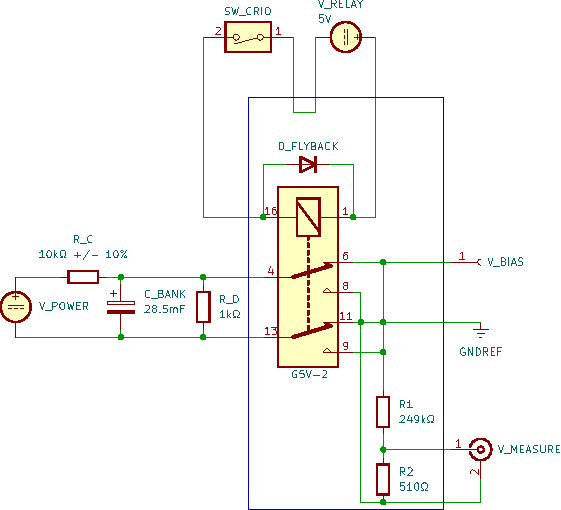
\includegraphics{chapter_pa_probe/figures/bias_polarity_switch_circuit.pdf}
    \caption[*PA Probe Biasing Circuit]{Diagram of the biasing circuit for the PA probe. The charging resistor, $R_c$, let's us charge the capacitor bank without having a short circuit while the discharge resistor, $R_d$, allows for quick changes the bias on the capacitor bank when remotely changing the power supply voltage, $V_b$. Since the capacitors are electrolytic the relay system works to change which side of the capacitor bank is connected to ground. The capacitor bank voltage is measured through a large voltage divider consisting of resistors $R_1$ and $R_2$.}
    \label{fig:pa_bias_circuit}
\end{figure}

A diagram of the biasing circuit can be found in figure \ref{fig:pa_bias_circuit} and an image in \ref{fig:pa_bias_image}. For each shot, all of the tips on the probe are biased to a single voltage relative to ground so we use a large capacitor bank to supply the tips with sufficient current while allowing for remote control using a relay system for changing bias polarity.

% \subsubsection{Principles of operation}

% The PA bias circuit system operates on the same principles as the multi-tip probe where we want a large charge reservoir to balance the current drawn by the probe and to keep the bias applied to the tip constant.

% \paragraph{Charging}

Charging is done through $V_{\text{power}}$, a remotely operated power supply that can go up to 250 V, 375 mA. We charge the capacitors through a charging resistor which reduces the maximum current allowed to flow from the power supply which protects it and the capacitors.

% \paragraph{Discharging}

To reduce the voltage to the tips quickly and for safety purposes we use a discharge resistor. This gives an RC time of approximately 30 seconds which, relative to a shot period of three minutes, is short enough to change the bias voltage to a new value between shots.

% \paragraph{Swapping polarity}

For sufficient capacitance, low inductance, and high voltage rating, we use electrolytic capacitors. As these capacitors are polarized and must be charged unidirectionally, we use a relay system to change the polarity of the bias voltage relative to ground.

% \subsubsection{How do we do this}

\begin{figure}
    \centering
    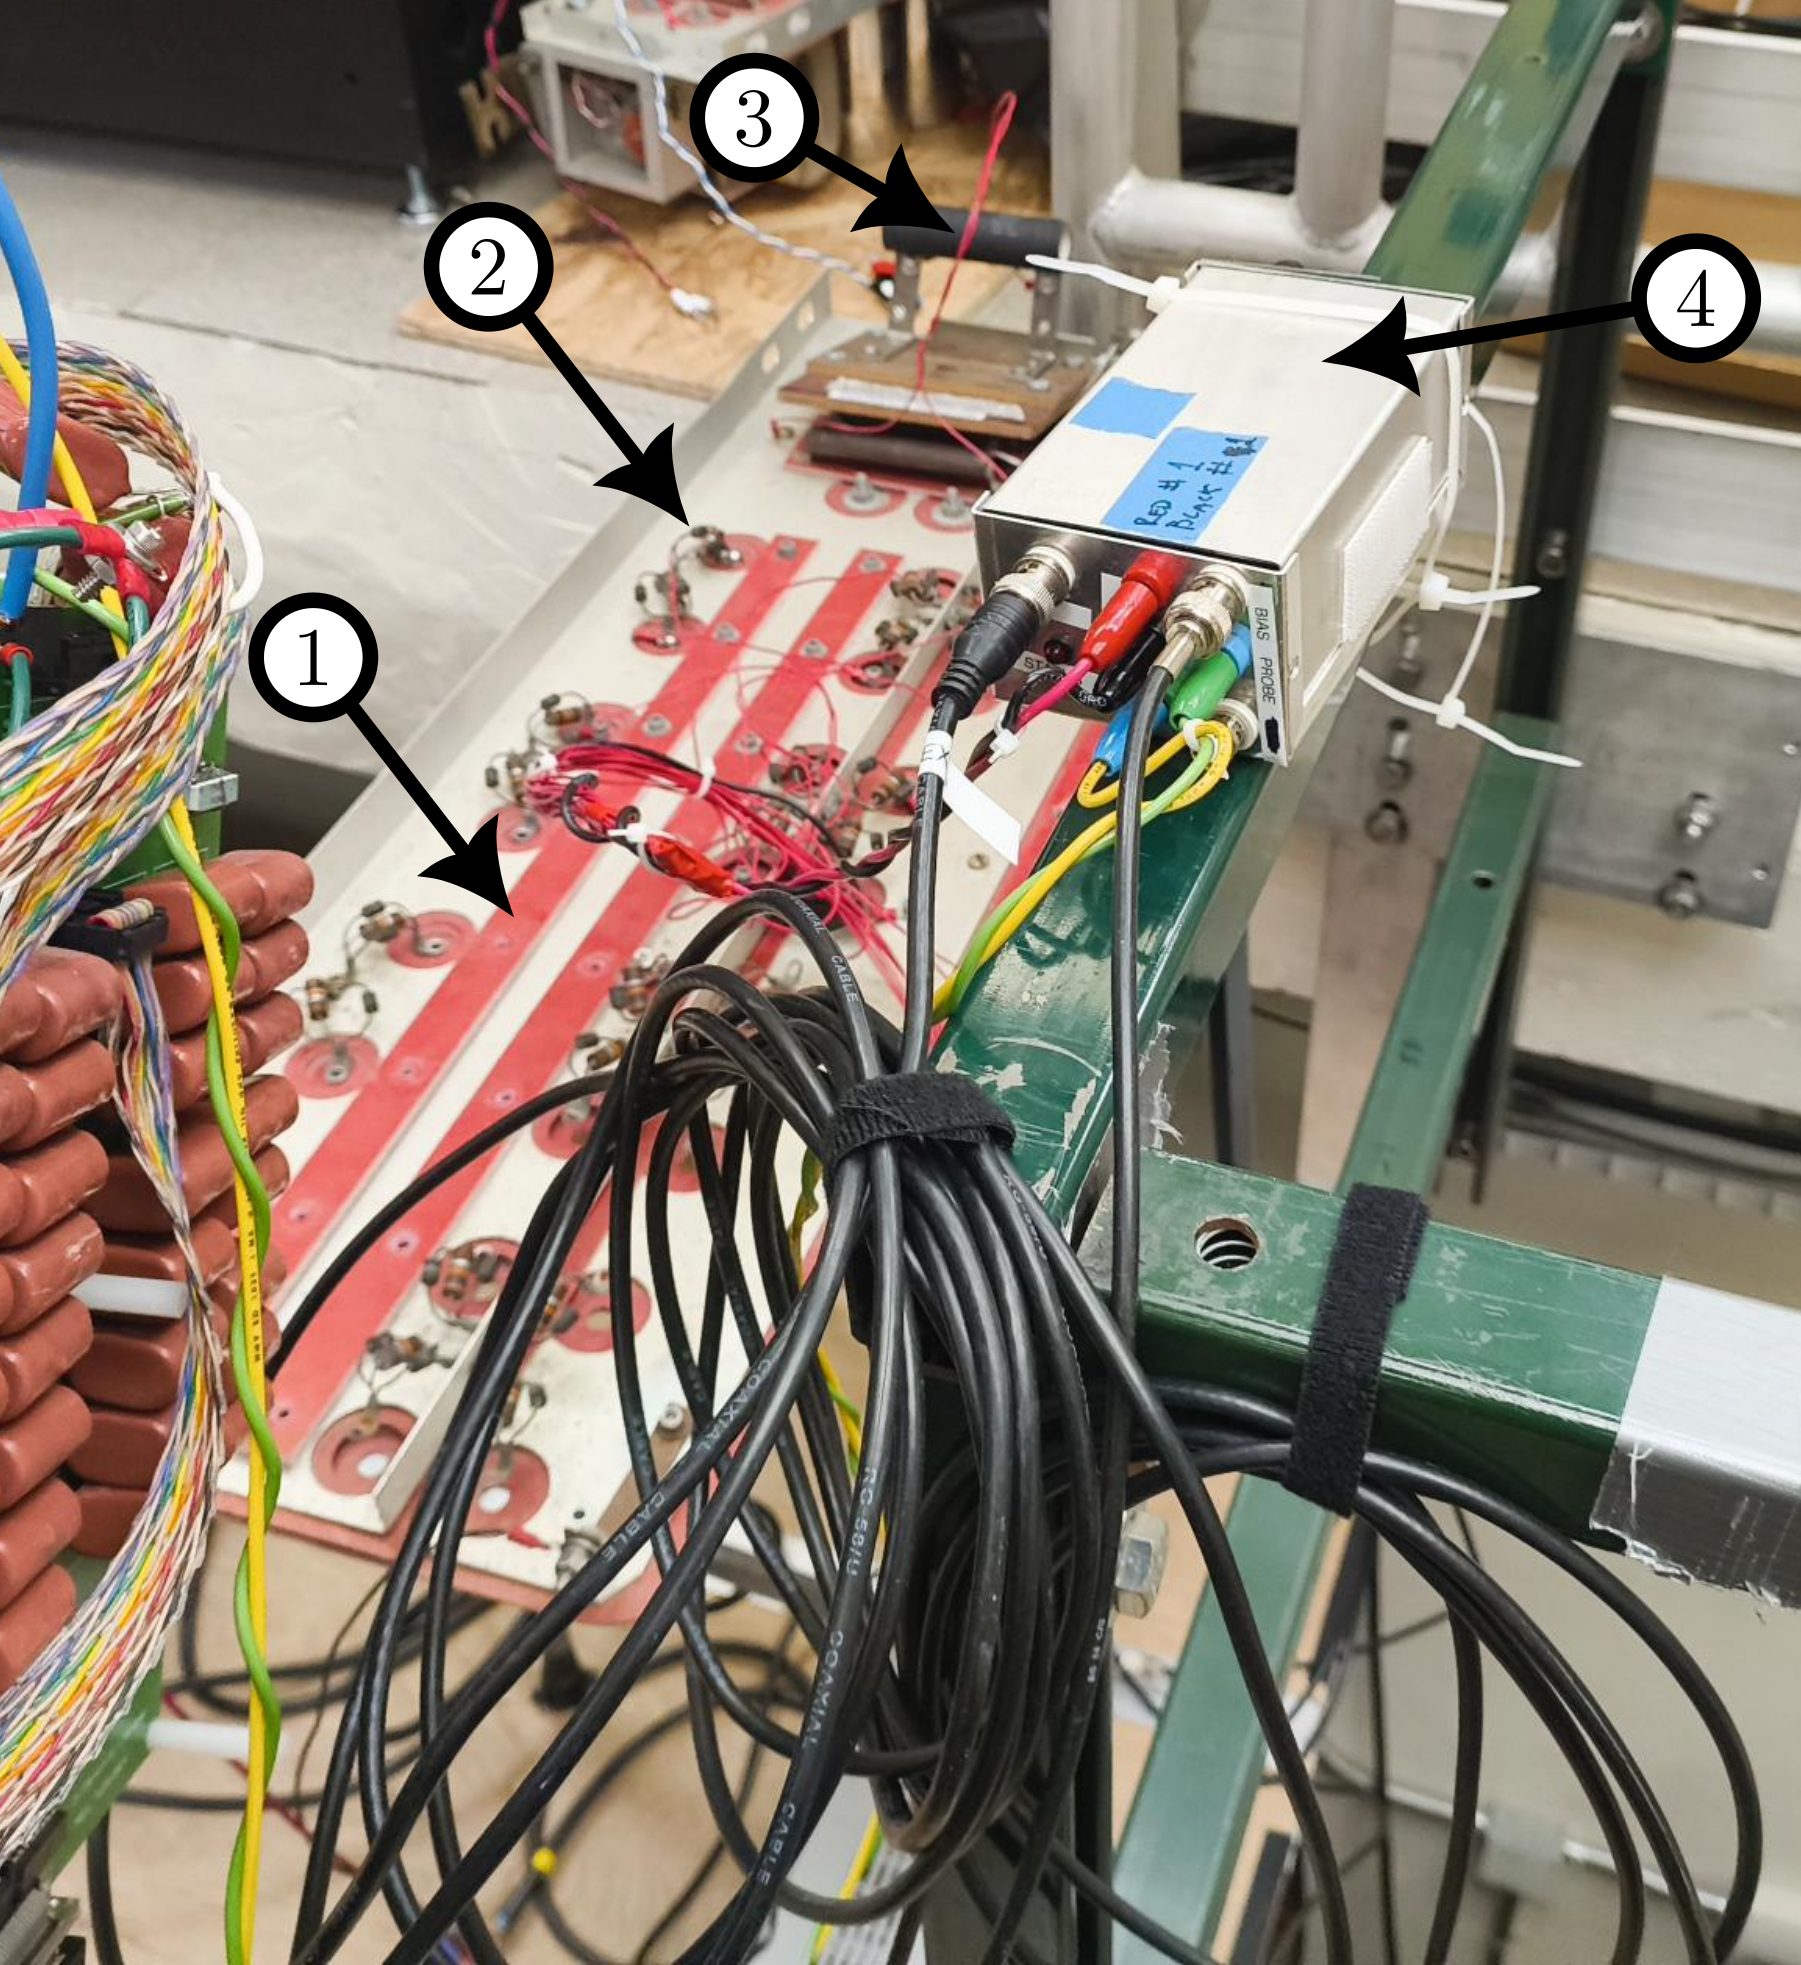
\includegraphics{chapter_pa_probe/figures/cap_bank_picture.png}
    \caption[*PA Capacitor Bank Image]{Image of the capacitor bank for the PA probe. The bank consists of two plates to apply external bias (1) which then charges the capacitors through a charging resistor (2). To discharge the capacitor we use a carborundum high power resistor (3). The polarity of the bias is set by a relay circuit (4).}
    \label{fig:pa_bias_image}
\end{figure}

% Now that we've discussed the principles of how this thing should operate, let's dive into some of the details of really getting it built and working. An image of the system can be seen in figure \ref{fig:pa_bias_image}.

% \paragraph{Cannibalization}

% A classic experimental technique is that of cannibalization; i.e. using parts from old systems that don't work quite like we want! In this case we've used a large capacitor bank, 1 in fig. \ref{fig:pa_bias_image}, consisting of many individual electrolytic capacitors which are connected to plates for positive and negative bias. Between the positive bias plate and the positive terminal is a charging resistor and also a diode for capacitor protection, 2 in fig. \ref{fig:pa_bias_image}.

% \paragraph{Discharging}

% We use a high power resistor, 3 in fig. \ref{fig:pa_bias_image}, to discharge the capacitor bank without burning up the resistor.

% \paragraph{Reducing voltage drop due to inductance}

% Since we want to keep the bias voltage applied to the tip constant, we've taken a few steps to make that happen.

% \subparagraph{Twisting Wires}

% One such solution is twisting all pairs of wires between the capacitor bank and the relay system and similarly between the relay and the board where the sense resistors are. Additionally instead of just having a single wire from the capacitors in the bank we've made it multi-stranded such that each capacitor has it's own wire to help reduce inductance.

% \subparagraph{Adding cap next to board}

% We've also put a capacitor just before the sense resistor board that, while being low capacitance, helps keep the voltage constant by storing charge for biasing right where the probe samples the bias.

% \paragraph{Reversing polarity}

% We use a Double-Pole Double-Throw relay to select which side of the capacitor bank goes to ground. This is controlled remotely using a cRIO switch. Unfortunately we found that sometimes the relay breaks and if not caught quickly, leads to many wasted shots.

% \subparagraph{Why does the relay break}

% We hypothesize that the relay breaks because of high transient current/voltage during switching. If the capacitor bank has some charge on it (say 25 V), there must be some current needed to shift the bias relative to ground because of parasitic capacitance with the lab. Additionally the capacitor we've placed at the sense resistor boards is a source of energy that could destroy the relay.

% \subparagraph{How do we fix this problem}

% We've found that if we be careful about when we change from negative to positive bias leads to a longer relay lifetime. This is coded into the control interface such that there is a discharge delay which is dependent on the initial bias applied to the capacitor bank.

% \subsubsection{Calibration}

% This power supply was calibrated in the same way as described in section \ref{ss2:multitip_remote_bias}.

\subsection{Probe Circuit}

The probe circuit model can be seen in figure \ref{fig:pa_tip_circuit_diagram} which is similar to \ref{fig:multitip_simple_tip_circuit}. We use the same circuit setup as done with the final iteration of the multi-tip probe by using differential digitizers and a secondary set of parallel circuits not shown in the diagram.

\begin{figure}
    \centering
    \begin{circuitikz}[american]
        % Shell signal, core signal, and core noise circuits.
        % Start by drawing shell signal circuit.
        \draw (0,0) node[left](bias){$V_b$} to[R=$R_{ss}$, name=Rss, i=$I_{ss}$, o-*] ++(2.5,0)
        coordinate(shell split) to[R=$R_{ws}$, name=Rws, i<=$I_{ps} + I_{pn}$] ++(5,0)
        to[short, -o, name=shell mid probe] ++(3,0) node[right](shell plasma){$V_{ps} + \tilde{V}_m$}
        (shell split) -- ++(0,-1) coordinate(shell core split)
        to[C, *-] ++(0,-1)
        to[R=$R_{ds}$, name=Rds, i>_=$I_{ds}$] ++(0,-1.5)
        to[vsource, invert, v_=$V_c$] ++(0,-1.5)
        node[tlground]{}
        % Draw core signal.
        (shell core split) -- ++(1,0) 
        coordinate(core noise split) to[short, *-] (core noise split -| Rws.west) 
        to[R=$R_{sc}$, name=Rsc] 
        (core noise split -| Rws.east) to[short, i=$I_{sc}$] ++(1,0)
        coordinate(core split) to[R=$R_{wc}$, name=Rwc, *-o, i<=$I_{pc} + I_{pn}$] (core split -| shell plasma.west) 
        node[right](core plasma){$V_{pc} + \tilde{V}_n$} 
        (core split) to[C] ++(0, -1)
        to[R=$R_{dc}$, name=Rds, i>_=$I_{dc}$] ++(0,-1.5)
        to[vsource, invert, v_=$V_c$] ++(0,-1.5)
        node[tlground](core ground){}
        % Draw core noise.
        (core noise split) -- ([yshift=-1cm] core noise split |- core ground)
        coordinate(noise turn) -- (noise turn -| Rws.west)
        to[R=$R_{sn}$, name=Rsn]
        (noise turn -| Rws.east) to[short, i=$I_{sn}$] (noise turn -| core split)
        coordinate(noise split) to[R=$R_{wn}$, name=Rwn, *-o, i<=$I_{pn}$] (noise split -| shell plasma.west)
        node[right](noise plasma){$V_{pn}$} 
        (noise split) to[C] ++(0, -1)
        to[R=$R_{dn}$, name=Rdn, i>_=$I_{dn}$] ++(0,-1.5)
        to[vsource, invert, v_=$V_c$] ++(0,-1.5)
        node[tlground](noise ground){}
        ;
        % Draw shell noise.
        \draw ([yshift=-1cm] bias |- noise ground) node[left](moise bias){$V_b$} to[R=$R_{sm}$, name=Rsm, i=$I_{sm}$, o-*] (moise bias -| shell split)
        coordinate(moise split) to[short, i<=$I_{pn}$] (moise split -| Rws.west)
        to[R=$R_{wm}$, name=Rsm]
        (moise split -| Rws.east) to[short, -o]
        (moise split -| shell plasma.west) node[right](moise plasma){$V_{pm}$}
        (moise split) to[C] ++(0,-1)
        to[R=$R_{dm}$, name=Rdm, i>_=$I_{dm}$] ++(0,-1.5)
        to[vsource, invert, v_=$V_c$] ++(0,-1.5)
        node[tlground]{}
        ;
        % \path (shell mid probe) \coord(shell mid probe);
    \end{circuitikz}
    \caption[*PA Probe Tip Circuit Diagram]{PA circuit model for a single tip with non-static digitizer ground. The shell and core (subscripts $s$ and $c$) both have independent noises ($m$ and $n$ respectively). The digitizers, which measure the voltage across $R_{d\_}$, haven't been drawn to reduce clutter. This model assumes each digitizer is connected to changing ground acting like the chassis of the digitizer changing voltage.}
    \label{fig:pa_tip_circuit_diagram}
\end{figure}

% \subsubsection{Single-ended measurement}

% There are a few different ways we could go about measuring the signals coming from the PA probe. One option is something like an oscilloscope which, while great at having a high sample rate, also has the major issue of grounding the signal through the measurement and the measurment is relative to the oscilloscope ground.

% \paragraph{TREX cells}

% These digitizers act similarly to an oscilloscope with many channels where the ground is shared between all measurement channels.

% \paragraph{Problems}

% Since the ground of the measurement is shared between all of the measurements, common mode noise very easily enters the measurement leading to wild oscillations when the capacitor bank for the drive coils triggers. Ideally subtracting off the noise measurement would correct for this but because of slight differences in circuit resistances and measurement gains, the subtraction does not sufficiently remove noise leaving an SNR of less than 0.1.

% \paragraph{Next steps}

% After a fair amount of time working to calibrate the circuit and remove noise, we decided to move onto use a different set of digitizers that use a differential measurement.

% \subsubsection{Differential measurement}

% Using the ACQ2X06s, a set of differential digitizers, we can measure the difference between two signals instead of the difference between a signal and ground so we've changed the circuit to best account for that. The circuit components are the same as seen in \ref{fig:pa_tip_circuit_diagram} but with an additional parallel circuit.

% \paragraph{Parallel circuitry}

% Instead of having a single set of resistors and a high-pass capacitor for a tip, we've doubled the circuits on the sense resistor board as can be seen in the middle blue box in figure \ref{fig:pa_grounding_diagram}. For the shell noise and signal it's a simple case of just having another set that is parallel to the shell measurement. For the core, since it is connected to the shell circuit just prior to $R_{sc}$ and $R_{sn}$, the parallel circuit is connected at the same point.

% By using this parallel circuitry we drastically reduce the noise in the measurement which helps a lot.

% \begin{table}
%     \caption{Probe circuit component values}
% \end{table}

% \subsubsection{Grounding Techniques}

% Good grounding leads to a happy diagnostic. Bad grounding leads to an unhappy graduate student.

Since we have immense amounts of current flowing when triggering the drive coils, capacitive and inductive coupling can occur leading to a significant amount of potential noise in the digitized measurements. This can be ameliorated by grounding the circuit such that currents only have a single path to ground \cite{Horowitz_Hill_1989}. After a significant amount of testing, the grounding scheme shown in figure \ref{fig:pa_grounding_diagram} has shown to be very noise resilient.

% \paragraph{Types of grounds on the ACQ}

% The ACQ2X06 digitizers (where $\text{X} \in \{1, 2\}$) have two types of ground. The first comes from the power cable plugged into the digitizer which we'll call the `chassis' ground (as can be seen in figure \ref{fig:pa_grounding_diagram}). This ground is not directly used during measurement but is instead for safety in case of arcs. The second ground is that of the onboard differential amplifier (called the `0V' ground). This ground sets the limits of the amplifier and by tying the probe circuit ground to this ground, noise between the probe circuit and amplifier can be removed. The `chassis' and `0V' grounds are connected by a high resistance so that the `0V' ground does not float away but also is decoupled.

% \paragraph{Routing grounds}

% Figuring out how to put all the grounds together was a long and arduous process. After much trial and error, we've come up with the solution found in \ref{fig:pa_grounding_diagram}. The entire system is powered by an isolation transformer, \texttt{T1}. This removes the building ground from the circuit and let's us optionally choose a different ground (we've neglected to attach a grounding wire at the transformer). Instead we ground the sytem through the `chassis' ground of the digitizers and also at the sense resistor board to tie the base of the resistor dividers. The base of the resistor dividers is also directly connected to the `0V' ground which makes the divider measurements move with the opamp making the signal have low noise.

\begin{figure}
    \centering
    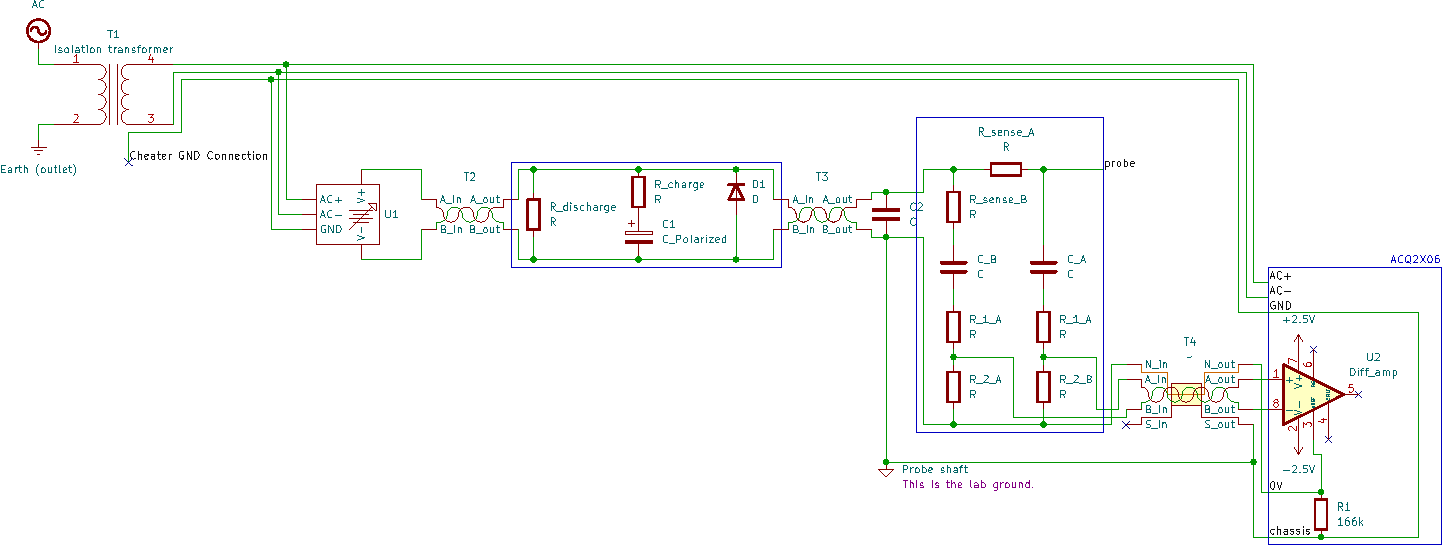
\includegraphics[width=\textwidth]{chapter_pa_probe/figures/simple_pa_circuit_no_page.pdf}
    \caption[PA Probe Grounding Diagram]{Schematic showing the ground paths for the PA probe. Power to the system comes from an isolation transformer, \texttt{T1}, which powers a controllable power supply, \texttt{U1}, and the digitizer, \texttt{ACQ2X06}. The bias capacitors, \texttt{C1}, are charged and the outgoing bias is applied to the probe board which contains the sense resistors, high-pass capacitor, and dividers (\texttt{R\_sense}, \texttt{C}, and (\texttt{R\_1}, \texttt{R\_2})). Outputs from the board are then measured by the digitizer. The grounding wire is connected to the probe shaft which is then connected to the machine.}
    \label{fig:pa_grounding_diagram}
\end{figure}

% \subsubsection{Swapping current paths}
% \label{ss2:pa_swapping_current_paths}

Since the circuit elements are not all of equal value, slight deviations in resistance can lead to artifacts in the derived probe currents and voltages. To correct for this effect we have implemented a circuit that swaps the path the current the core receives from the plasma between the $c$ subscript and $n$ subscript in figure \ref{fig:pa_tip_circuit_diagram}. Since the derivation of the core current requires the subtraction of $I_{dc}$ and $I_{dn}$ which have a large common mode component, this swapping helps with common mode noise rejection.

If our circuit components were ideal, each element would act the same as that same element for other tips. Since there is some variation in resistance between sense resistors and divider resistors, it's useful to have two current paths for the core measurements.

% \paragraph{Why do we want to do this}

% The current collected by the core is quite small and the raw voltage measurement, $V_{dc}$, is dominated by the shell current by a factor of around 20. Now $R_{sc}$ ($R_{sn}$) and $R_{dc}$ ($R_{dn}$) make a resistor divider that divides down the core signal (noise) measurement and then the core signal and noise measurements, $V_{dc}$ and $V_{dn}$, are subtracted to get the core signal.

% \subparagraph{Deviations in resistance}

% If the resistors in the circuit are different though, the subtraction does not fully remove the shell signal. This causes the derived core voltage and current to be either anomalously high or low compared to it's actual value.

% \subparagraph{Correcting for this}

% The reason the shell leaks into the core measurement is because of the different divider ratios between the core signal and noise. If we swap the resistors for those two signals though, we can see the effect of both adding shell signal and subtracting shell signal. We can then average the signal between the original path and the swapped path to remove the shell contribution.

% \paragraph{Circuitry to do this}

% The circuitry we use can be seen in figure \ref{fig:pa_swap_image} and the corresponding schematic in figure \ref{fig:pa_swap_circuit}. The circuit has a number of components used for isolating the CompactRIO (CRIO) from the circuit and also keeping current through the CRIO to a minimum.

% \subparagraph{Only swap core signal and noise}

% As we are trying to remove the influence of the different core noise and shell circuits, we only want to swap those two lines. The shell signal and noise are minimally affected by the core and the small resistor differences matter little.

% \subparagraph{Many relays}

% Each tip needs it's core measurements swapped so in total we have 12 relays. This means that we require a sufficient amount of current for all these relays and thus want to isolate the switching system from the CRIO which is low power.

% \subparagraph{Remote control}

% To control this switching system, we isolate the CRIO using an opto-isolator and use a switch in the CRIO that we can control via LabView. Since the signals we are switching are connected to the bias capacitor bank, we want to keep these high voltage high capacitance lines far away from the expensive CRIO components.

\begin{figure}
    \centering
    \begin{subfigure}{\textwidth}
    \centering
        
    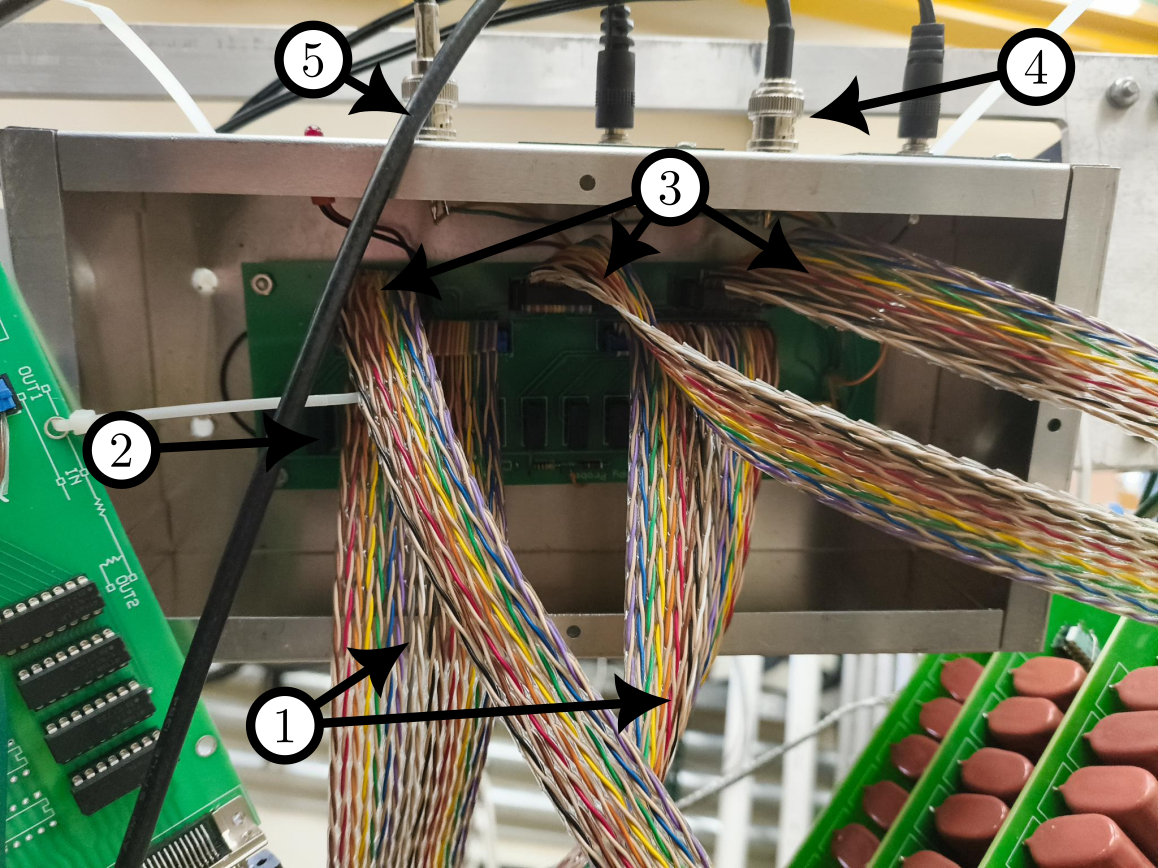
\includegraphics{chapter_pa_probe/figures/swap_box_image.png}
    \caption{Image of the swapping circuit}
    \label{fig:pa_swap_image}
    \end{subfigure}

    \begin{subfigure}{\textwidth}
    \centering
    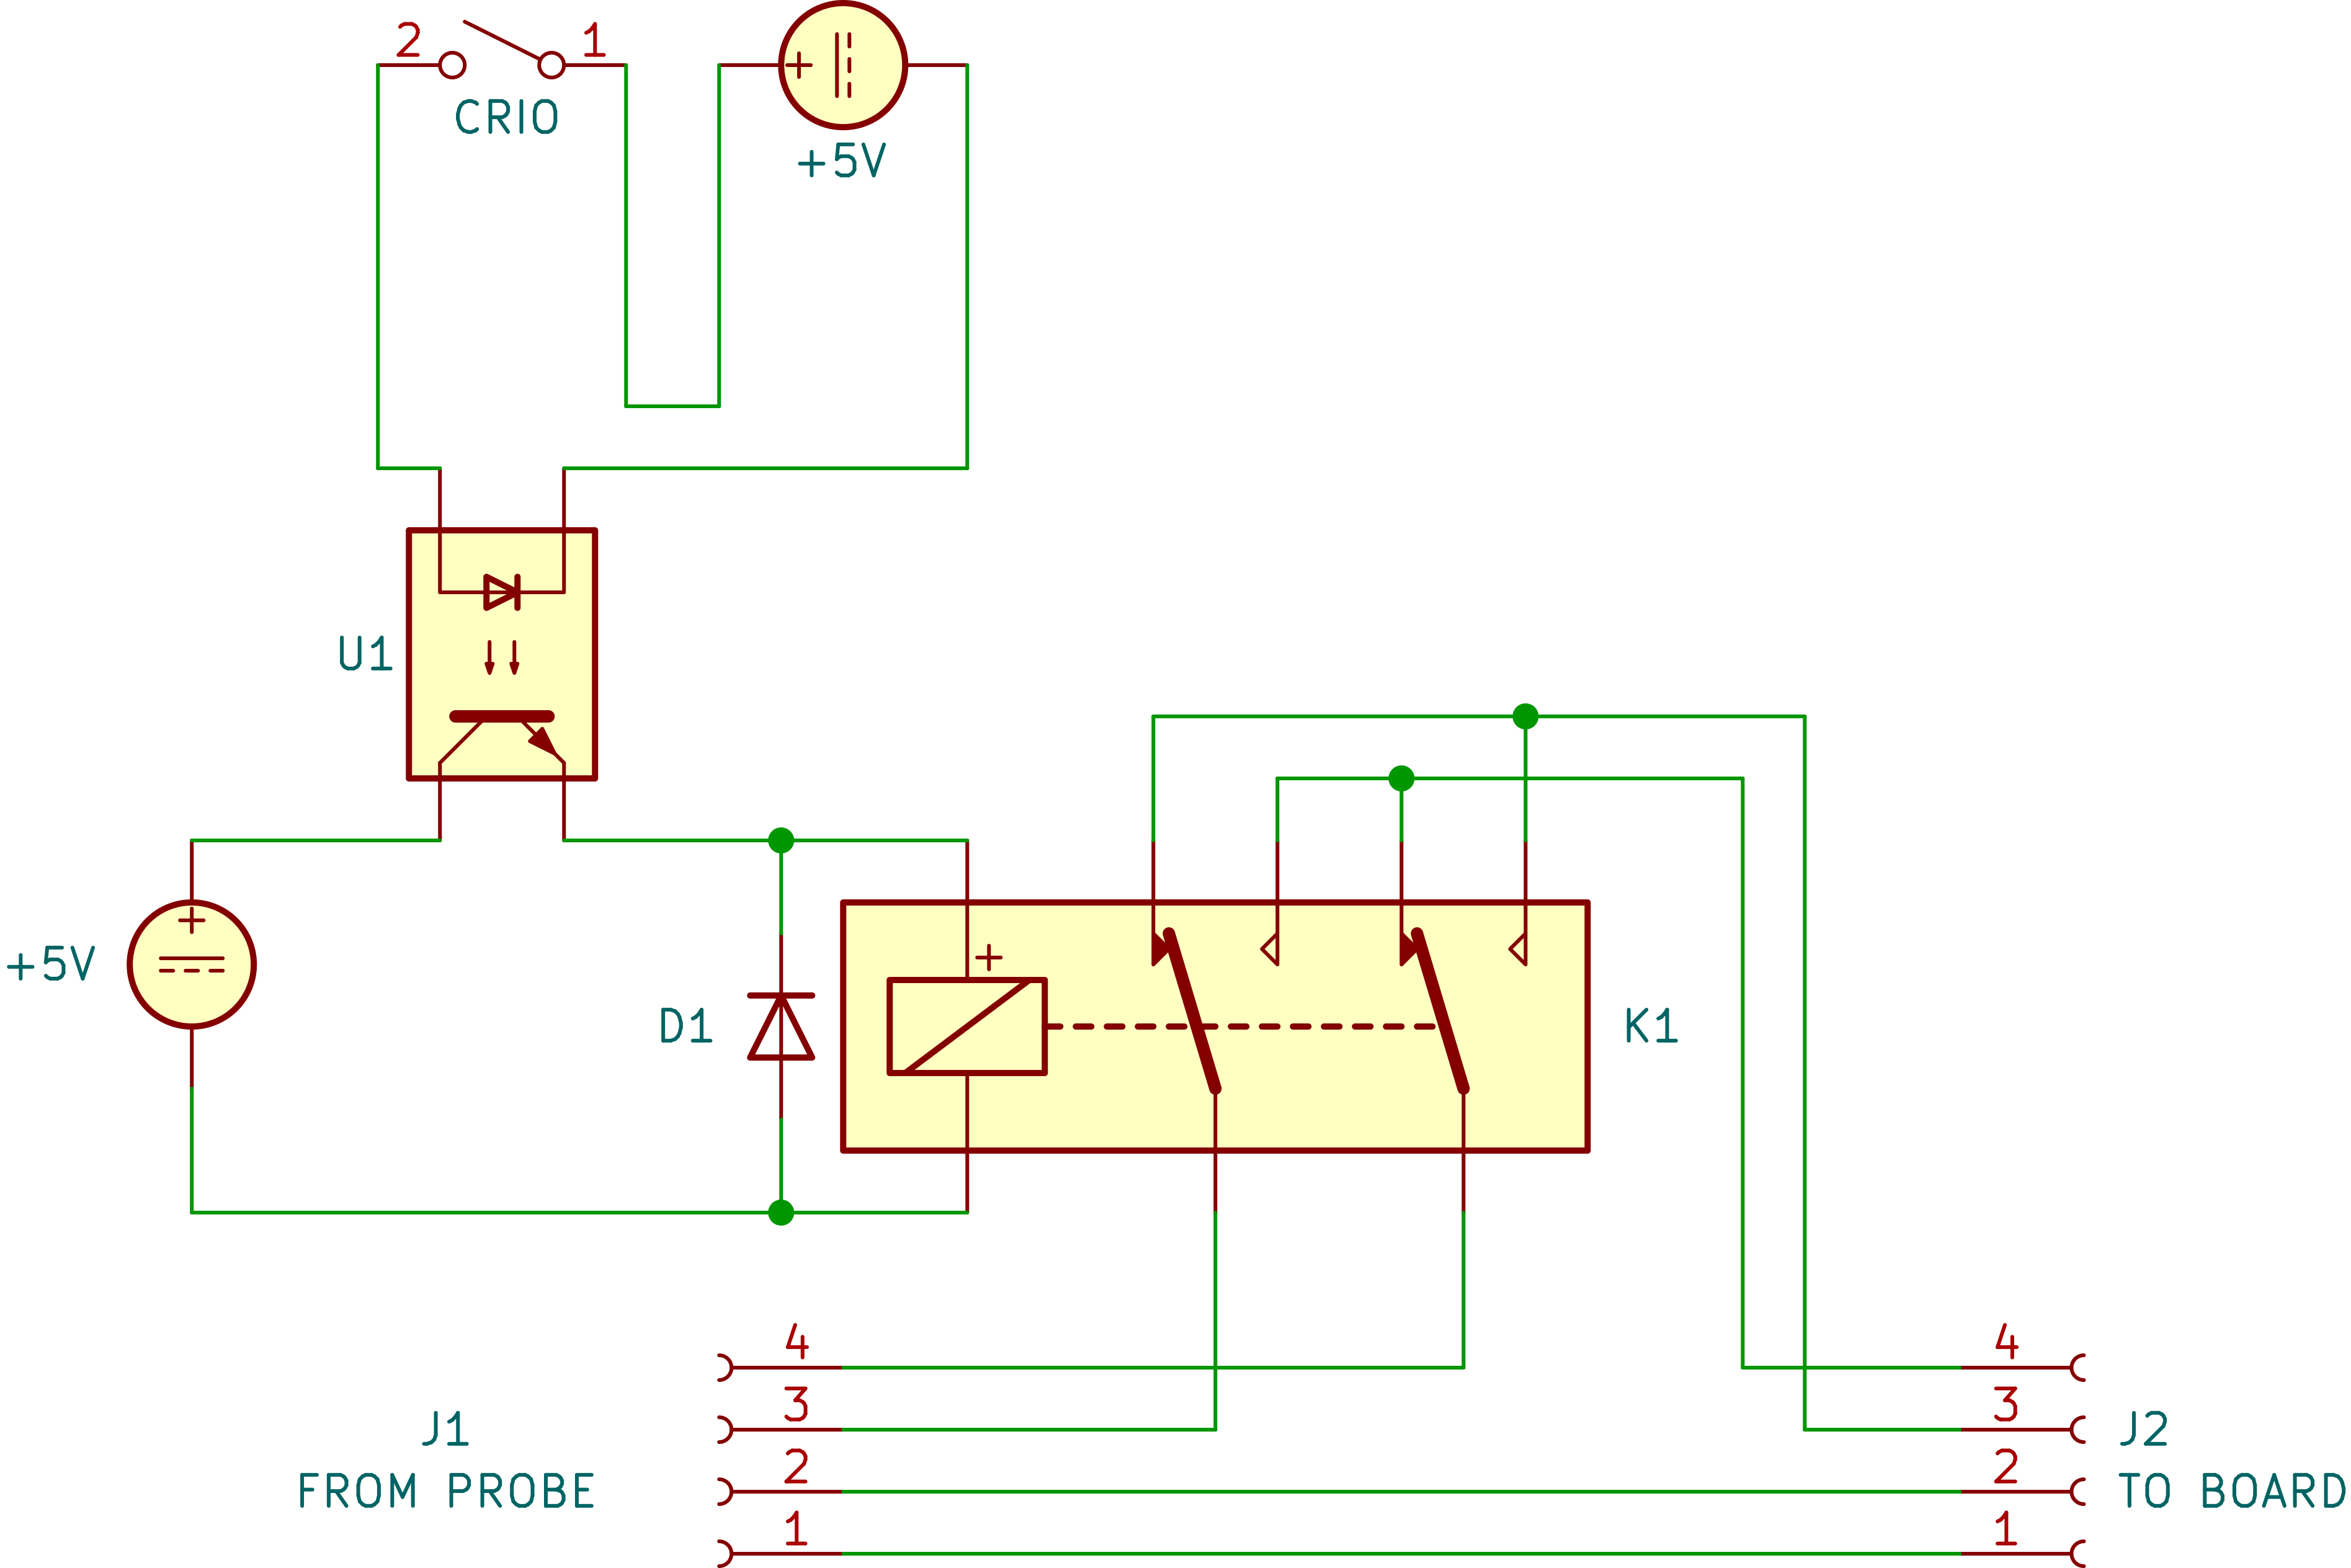
\includegraphics{chapter_pa_probe/figures/core_path_swapping_circuit.png}
    \caption{Diagram of the swapping circuit}
    \label{fig:pa_swap_circuit}
    \end{subfigure}
    \caption{An image and diagram of the circuit used for swapping the connection to the core between two circuit paths. The signals from the probe (1) \texttt{J1} enter the circuit and the core signals \texttt{3}, \texttt{4} pass through a relay (2) \texttt{K1}. This may result in \texttt{3} and \texttt{4} being swapped when leaving the probe (3) \texttt{J2}. The relay is controlled via the CompactRIO (5) \texttt{CRIO} and the relay status is measured using a digitizer (4).}
\end{figure}

% \paragraph{How does this change results}

Figure \ref{fig:pa_swap_effect} shows the difference between the un-swapped (circles) and swapped (squares) core measurements. It is especially clear in tips 2, 6, and 10 where the un-swapped measurements are far higher than the swapped because the shell is either adding or subtracting from the signal. By averaging these two options, as described in \ref{ss2:pa_averaging_relay}, we can correct for this problem.

\begin{figure}
    \centering
    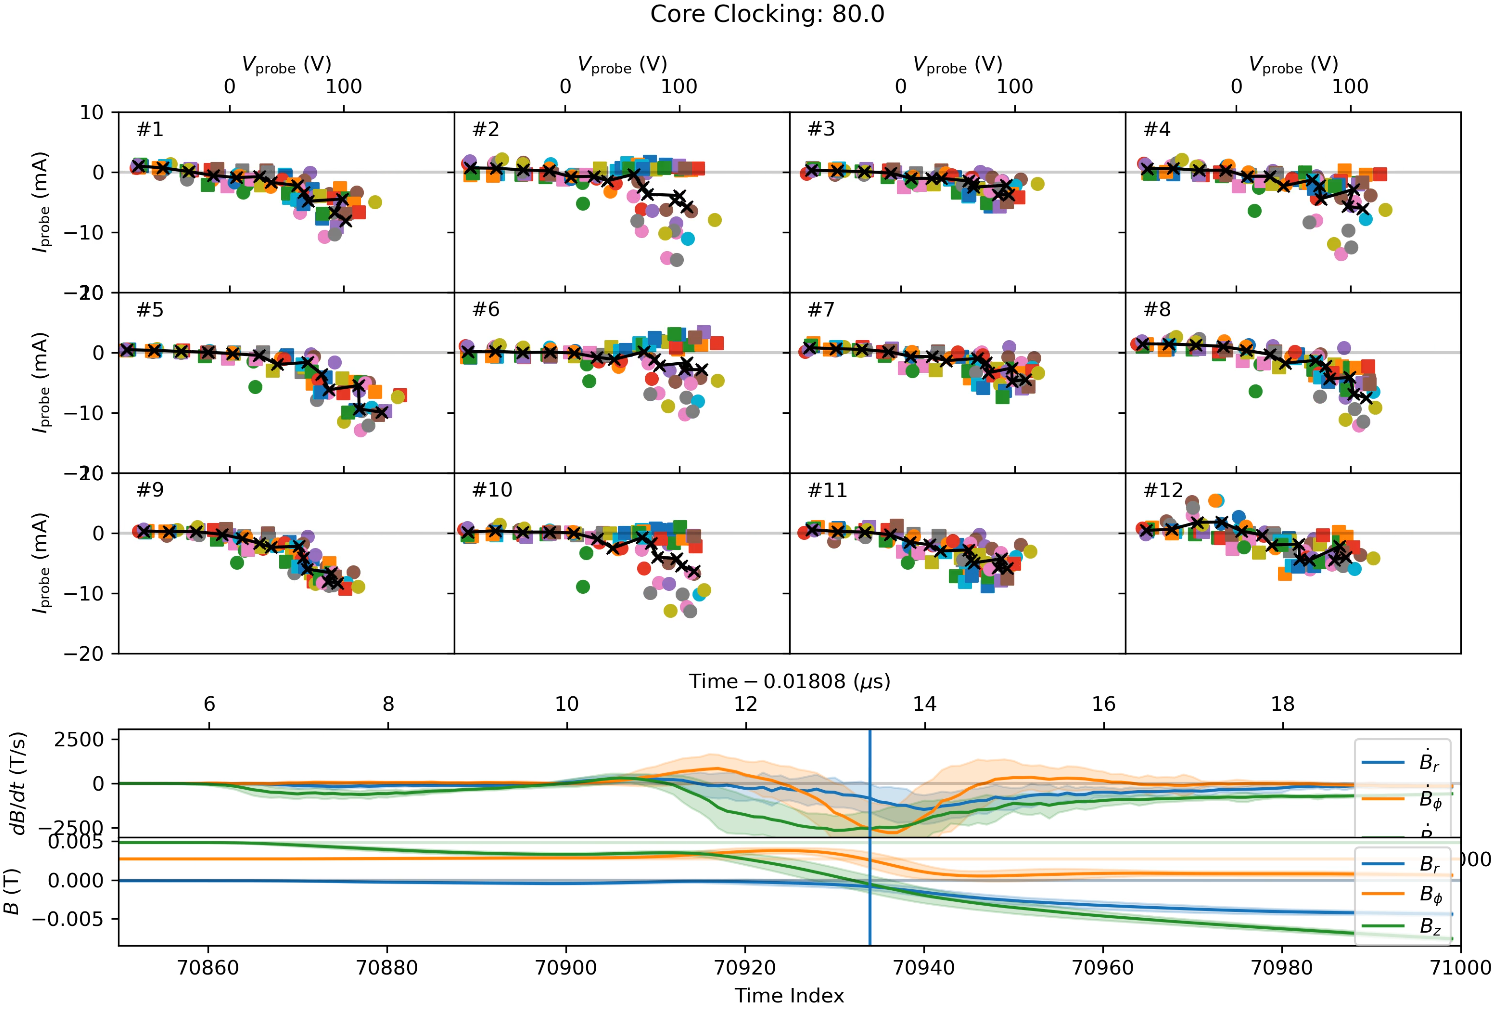
\includegraphics[width=\textwidth]{chapter_pa_probe/figures/example_core_swap_effect.png}
    \caption{Time frame for core movie of IV with separation between relay. These are the core tip's IV-characteristics derived from the digitizer measurements. Each shot is a separate colored scatter point with un-swapped being circles and swapped being squares. The relay averaged solution consists of black x's. The bottom panels show the measured magnetic field evolution at the location of the PA probe. The data shown is at the time when $B_z = 0$.}
    \label{fig:pa_swap_effect}
\end{figure}

% \subsubsection{Circuit Solution}

The circuit for the PA probe tips, figure \ref{fig:pa_tip_circuit_diagram}, acts similarly as that of the $T_e$ probe, figure \ref{fig:multitip_tip_circuit_w_noise}. The bias is input as $V_b$ and passes through a sense resistor which acts to bring the probe bias closer to the plasma floating potential (where the current from the plasma to the probe is 0). The core of each tip is attached to the shell circuit to minimize the generation of electric fields between the shell and core.

% \paragraph{Solution}

Much of this analysis is the same as that done for the multi-tip Langmuir probe in \ref{sss:multitip_probe_circuit} which result in the final equations for the probe potentials and currents, $V_{ps}$, $V_{pc}$, $I_{ps}$, and $I_{pc}$.

\begin{align*}
    % I_{pc} =& \frac{R_{dc} + R_{sc}}{R_{sc}} I_{dc} + \frac{R_{ds} (R_{sc} - R_{sn})}{R_{sc} R_{sn}} I_{ds} - \frac{R_{dn} + R_{sn}}{R_{sn}} I_{dn} \\
    % I_{ps} =& -\frac{R_{dc}}{R_{sc}} I_{dc} -\frac{R_{dn}}{R_{sn}} I_{dn} - \frac{R_{dm} + R_{sm}}{R_{sm}} I_{dm} + \left(1 + R_{ds} \left( \frac{1}{R_{sc}} + \frac{1}{R_{sn}} + \frac{1}{R_{ss}} \right) \right) I_{ds} \\
    % V_{pc} =& \frac{(R_{dc} (R_{sc}+R_{wc})+R_{sc} R_{wc})}{R_{sc}}I_{dc} -\frac{R_{ds} R_{wc}}{R_{sc}}I_{ds} +V_{b} \\
    % V_{ps} =& -\frac{R_{dc} R_{ws}}{R_{sc}}I_{dc} -\frac{R_{dn} R_{ws}}{R_{sn}}I_{dn} +\left(R_{ds} \left(\frac{R_{ws}}{R_{sc}}+\frac{R_{ws}}{R_{sn}}+\frac{R_{ws}}{R_{ss}}+1\right)+R_{ws}\right)I_{ds} +V_{b} \\
    I_{ps} =& - \frac{I_{dc} R_{dc}}{R_{sc}} + I_{dm} \left(- \frac{R_{dm}}{R_{ss}} - \frac{R_{sm}}{R_{ss}}\right) \\
    &+ I_{dn} \left(\frac{R_{dn} R_{sm}}{R_{sn} R_{ss}} - \frac{2 R_{dn}}{R_{sn}} + \frac{R_{sm}}{R_{ss}} - 1\right) \\
    &+ I_{ds} \left(- \frac{R_{ds} R_{sm}}{R_{sn} R_{ss}} + \frac{R_{ds}}{R_{ss}} + \frac{2 R_{ds}}{R_{sn}} + \frac{R_{ds}}{R_{sc}} + 1\right) \\
    V_{ps} =& - \frac{I_{dc} R_{dc} R_{ws}}{R_{sc}} + I_{dm} \left(- R_{dm} - \frac{R_{dm} R_{ws}}{R_{ss}} - R_{sm} - \frac{R_{sm} R_{ws}}{R_{ss}}\right) \\
    &+ I_{dn} \left(\frac{R_{dn} R_{sm}}{R_{sn}} + \frac{R_{dn} R_{sm} R_{ws}}{R_{sn} R_{ss}} - \frac{R_{dn} R_{ws}}{R_{sn}} + R_{sm} + \frac{R_{sm} R_{ws}}{R_{ss}}\right) \\
    &+ I_{ds} \bigg(- \frac{R_{ds} R_{sm}}{R_{sn}} - \frac{R_{ds} R_{sm} R_{ws}}{R_{sn} R_{ss}} + R_{ds} \\
    &\qquad+ \frac{R_{ds} R_{ws}}{R_{ss}} + \frac{R_{ds} R_{ws}}{R_{sn}} + \frac{R_{ds} R_{ws}}{R_{sc}} + R_{ws}\bigg) \\
    I_{pc} =& \frac{I_{dc} R_{sn} \left(R_{dc} + R_{sc}\right) - I_{dn} R_{sc} \left(R_{dn} + R_{sn}\right) + I_{ds} R_{ds} \left(R_{sc} - R_{sn}\right)}{R_{sc} R_{sn}} \\
    V_{pc} =& I_{dc} \left(R_{dc} + \frac{R_{dc} R_{wc}}{R_{sc}} + R_{wc}\right) + I_{dm} \left(- R_{dm} - R_{sm}\right) \\
    &+ I_{dn} \left(\frac{R_{dn} R_{sm}}{R_{sn}} + R_{sm}\right) \\
    &+ I_{ds} \left(- \frac{R_{ds} R_{sm}}{R_{sn}} - \frac{R_{ds} R_{wc}}{R_{sc}}\right)
\end{align*}

% \paragraph{Assumptions}

% Here we have the same assumption of noise coming from a changing measurement ground but we now can account for a second source of noise which is extraneous current flowing down the probe wires due to coupling or other strange effects. We've also assumed, similar to previously, that the high pass capacitors change too slowly during a shot for their charge to matter.

% \subsubsection{Calibration}

Calibration of the PA probe is done very similarly to that of the multi-tip Langmuir probe, \ref{sss:multitip_probe_circuit}. During the initial plasma equilibrium, the plasma is quite isotropic and along with the isotropic collection of the shells, we can calibrate the relative areas between each shell using the ion saturation current. Similarly, the wire resistances can be calibrated by using points on the exponential in the initial equilibrium.

% \paragraph{Calibrating on the exponential}

% \paragraph{Rotation calibration}

Although the initial equilibrium is quite isotropic, there is some flow from the plasma guns and cross-field diffusion of the plasma to higher radii. Thus to correct for these issues we calibrate the same core parameters as the shell by rotating the probe between shots such that each direction is covered by different tips. Then we can use the different shots with tips in the same direction in both the ion saturation region and on the exponential to get the core wire resistance and area.

% \subsubsection{The path to ground}

% \paragraph{Why do we have to care}

% \paragraph{How do we set it}

% \begin{figure}
%     \centering
    
%     \caption{Picture of circuit setup.}
%     \label{fig:pa_circuit_picture}
% \end{figure}

% \subsubsection{Capacitive coupling}

In the construction of this probe, each signal wire is twisted together with a noise wire, $s$ with $m$ and $c$ with $n$. This works well to make sure any noise due to capacitive coupling to the plasma was very similar between the signal and noise wires. Since they are twisted together, we found that there was a significant amount of capacitive coupling that the noise wires saw.

As can be seen in figure \ref{fig:pa_example_capacitive_coupling}, the shell noise (signal number 5) is approximately the derivative of the shell current (signal number 6) multiplied by some constant. This same feature exists for all tips but this coupling effect is far smaller for the core measurements since the difference in voltage between the $c$ and $n$ is very small.

\begin{figure}
    \centering
    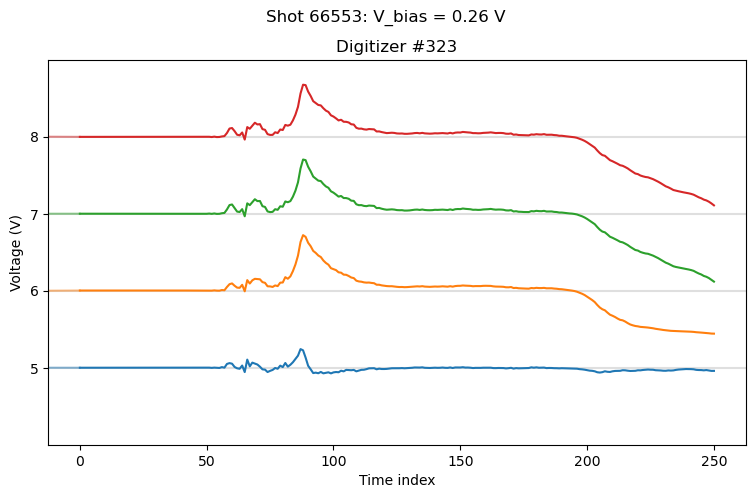
\includegraphics[width=\textwidth]{chapter_pa_probe/figures/example_raw_signal_trace_with_capacitive_coupling.png}
    \caption{Example of the raw signal measured by the digitizers. This signal is from tip \#2. Each signal has it's zero at the corresponding channel of the digitizer (i.e. the signal that starts at 5 V is really starting at 0 V but is offset by the channel number). Channel 5 is the shell noise wire, channel 6 is the shell signal wire, channel 7 is the core noise wire, and channel 8 is the core signal wire.}
    \label{fig:pa_example_capacitive_coupling}
\end{figure}

We believe this is due to the coupling acting as part of a passive differentiator. As can be seen in figure \ref{fig:passive_differentiator}, a passive differentiator is a resistor and capacitor acting as a divider. When $\overline{x} - g$ varies, at low frequency the capacitor acts as a break in the circuit leading to no voltage difference on $\overline{y}$ but at very high frequencies all the voltage is transferred to $\overline{y}$ since the capacitor acts as a short. The transfer function for this circuit can be written as
\begin{equation}
    \label{eq:passive_differentiator}
    \overline{Y} = \frac{sRC}{1 + sRC} \overline{X}
\end{equation}
where $\overline{X} = \overline{x} - g$ and $\overline{Y} = \overline{y} - g$ and $\overline{x}$, $\overline{y}$, and $g$ are the voltages at their respective nodes.

\begin{figure}
    \centering
    \begin{circuitikz}[american]
        \draw (0, 0) node[left]{$\overline{x}$}
        to[C=$C$, o-] ++(2, 0) coordinate(RC split)
        to[R=$R$] ++(0, -2) coordinate(gnd split)
        to[short, -o] (0, -2) node[left]{$g$}
        (RC split) to[short, -o] ++(1, 0) node[right]{$\overline{y}$}
        (gnd split) to[short, -o] ++(1, 0) node[right]{};
    \end{circuitikz}
    \caption{A passive RC differentiator. This figure is reproduced from \href{https://commons.wikimedia.org/wiki/File:Passive_differentiator_circuit_1.png}{Wikipedia}.}
    \label{fig:passive_differentiator}
\end{figure}

Figure \ref{fig:pa_tip_circuit_diagram_w_coupling} is the same as figure \ref{fig:pa_tip_circuit_diagram} except that we've added the capacitive coupling as a capacitor, $C_c$, and are only using the shell and shell noise components. As can be seen in the simplified circuit at the bottom of figure \ref{fig:pa_tip_circuit_diagram_w_coupling}, everything to the left of $C_c$ combines into a combination of the shell voltage measurement and the difference between the probe and plasma potentials. Elements to the right of $C_c$ lumped together becomes a resistor divider where $V_m$ is the output.

\begin{figure}
    \centering
    \begin{tikzpicture}
        % Paths, nodes and wires:
        \draw (11, 7.75) to[variable american resistor, l={$R_p$}] (11, 6.25);
        \draw (9, 8) to[american resistor, l={$R_w$}] (7.5, 8);
        \draw (6.5, 8) to[american resistor, l={$R_s$}] (5, 8);
        \draw (6.5, 6) to[american resistor, l={$R_s$}] (5, 6);
        \draw (9, 6) to[american resistor, l={$R_w$}] (7.5, 6);
        \draw (9.5, 7.75) to[capacitor, l={$C_c$}] (9.5, 6.25);
        \draw (7, 8.5) to[capacitor, l={$C_t$}] (7, 10);
        \draw (7, 4) to[capacitor, l={$C_t$}] (7, 5.5);
        \draw (7, 2) to[american resistor, l={$R_d$}] (7, 3.5);
        \draw (7, 10.5) to[american resistor, l={$R_d$}] (7, 12);
        \draw (4.5, 4.5) to[capacitor, l={$C_b$}] (4.5, 6);
        \draw (4.5, 2.5) to[american voltage source, l={$V_b$}] (4.5, 4);
        \draw (11, 2.5) to[american voltage source, l={$V_p$}] (11, 4);
        \draw (7.5, 8) -- (6.5, 8);
        \draw (7, 8.5) -| (7, 8);
        \draw (7, 10.5) -| (7, 10);
        \draw (7, 12) -| (12.25, 2) -| (4.5, 2.5);
        \draw (4.5, 4.5) -| (4.5, 4);
        \draw (4.5, 6) -- (5, 6);
        \draw (5, 8) -- (4.5, 8) -| (4.5, 6);
        \draw (6.5, 6) -- (7.5, 6);
        \draw (7, 5.5) -| (7, 6);
        \draw (7, 4) -| (7, 3.5);
        \draw (9, 8) -| (11, 7.75);
        \draw (11, 6.25) -| (11, 4);
        \draw (11, 2.5) -| (11, 2);
        \draw (9.5, 8) -| (9.5, 7.75);
        \draw (9.5, 6.25) |- (9, 6);
        \draw (7, 10.5) to[voltmeter, l={$V_s$}] (8.5, 10.5);
        \draw (8.5, 12) -| (8.5, 10.5);
        \draw (7, 3.5) to[voltmeter, l={$V_m$}] (8.5, 3.5);
        \draw (8.5, 3.5) -| (8.5, 2);
        \path[draw={rgb,255:red,224;green,27;blue,36}, line width=2pt, -latex] (7.25, 1.75) -- (7.25, 1);
        \draw (4, -1.5) to[voltmeter, l={$V_s$}] (4, 0);
        \draw (12.75, -1.5) to[voltmeter, l_={$V_m$}] (12.75, 0);
        \draw (5.25, -1.5) to[american resistor, l={$R_d$}] (5.25, -0);
        \draw (6.5, -1.5) to[american resistor, l={$R_s$}] (6.5, -0);
        \draw (6.5, 0) to[american resistor, l={$R_w$}] (8, -0);
        \draw (8, 0) to[capacitor, l={$C_c$}] (9, -0);
        \draw (9, 0) to[american resistor, l={$R_w$}] (10.5, -0);
        \draw (10.5, -1.5) to[american resistor, l={$R_s$}] (10.5, -0);
        \draw (11.75, -1.5) to[american resistor, l={$R_d$}] (11.75, -0);
        \draw (8, -0) to[variable american resistor, l_={$R_p$}] (8, -1.5);
        \draw (4, -0) -- (6.5, -0);
        \draw (4, -3) -- (12.75, -3);
        \draw (10.5, -0) -- (12.75, -0);
        \draw (6.5, -3) -- (6.5, -1.5);
        \draw (10.5, -3) -- (10.5, -1.5);
        \draw (8, -3) to[american voltage source, l_={$V_p - V_b$}] (8, -1.5);
        \draw (4, -1.5) -| (4, -3);
        \draw (5.25, -1.5) -| (5.25, -3);
        \draw (11.75, -1.5) -| (11.75, -3);
        \draw (12.75, -1.5) -| (12.75, -3);
    \end{tikzpicture}
    \caption{The capacitive coupling of the shell signal and the shell noise which are coupled by capacitor $C_c$. The signals are measured via $V_n$ and $V_s$. The left side of the top circuit is the bias voltage ($V_b$) applied to the biasing capacitor ($C_b$). $R_p$ is the resistance of the plasma which is calculated from Ohm's law: $V_\text{probe} - V_\text{plasma} = I_\text{probe} R_\text{plasma}$. The $p$'s in $V_p$ and $R_p$ are for `plasma'. To achieve the bottom circuit, we've simplified the top circuit by combining voltage supplies and removing capacitances that are too large to play into the capacitive coupling effect we see.}
    \label{fig:pa_tip_circuit_diagram_w_coupling}
\end{figure}

% \paragraph{Magnitude of effect}

We are using very fine twisted pair wire with a wire diameter of 0.003 inches, a separation between wire centers of 0.003 inches, and insulating dielectric constant of 2.2. This gives a capacitance per meter of 84.2 pF / m. Using a sense resistance of 680 $\Omega$ we find that $RC \approx 0.11$ \textmu s. Since our signals are on the order of 0.1 \textmu s ($s \approxeq 6 \cdot 10^7$ rad/s) the magnitude of the coefficient in \ref{eq:passive_differentiator} is $\approx 0.8$.

% \paragraph{Removing effect}

% TODO: Update this.
As of this writing, the best way to take care of this effect is to ignore it. This is because the only reason we may want to remove this effect is if we want to extract the common mode noise to then remove from the signal. For the shell, the magnitude of the coupling on the noise signal can be up to 1/3rd of the shell signal whereas the common mode noise for the shell is far smaller (on the order of 1\%). For the core, since both the core signal and core noise have a very similar voltage, the capacitive coupling is very small and although the common mode noise is larger, the capacitive coupling is very small.

\section{Plasma Theory}

The PA probe is a novel diagnostic and an understanding of the plasma parameters that result in the measured IV-characteristics must be derived. The following two methods are based around either fitting all the tips at once by integrating the distribution function or fitting tips individually and later combining their results.

\subsection{All Tip Model}

This model operates to fit all the tips at once in the ion attracting/electron repelling regime where the probe potential is less than the plasma potential.

% \subsubsection{Plasma Distribution}

We assume that the plasma can be modeled as a drifting bi-Maxwellian for the electrons where the temperature parallel to the magnetic field, $\vb{B}$, is different than the temperature perpendicular to it. Let the drift velocity be $\vb{v_D}$. Then we can write our distribution function as the following:
\begin{equation}
    f_e(\vb{v}) = \left(\frac{e m_e}{2\pi}\right)^{3/2} \frac{n}{\sqrt{T_{e\perp}^2 T_{e\parallel}}} \exp\left[-\frac{e m_e}{2} \left(\frac{(\vb{v} - \vb{v_D})_\parallel^2}{T_{e\parallel}} + \frac{(\vb{v} - \vb{v_D})_\perp^2}{T_{e\perp}}\right)\right]
    \label{eq:drifting_bimaxwellian}
\end{equation}
where
\begin{align*}
    (\vb{v} - \vb{v_D})_\parallel^2 &= \left((\vb{v} - \vb{v_D}) \cdot \hat{b}\right)^2 \\
    (\vb{v} - \vb{v_D})_\perp^2 &= \left((\vb{v} - \vb{v_D}) - \left((\vb{v} - \vb{v_D}) \cdot \hat{b}\right) \hat{b} \right)^2.
\end{align*}

We assume the ions are isotropic but may drift. The ion temperature is minimally impactful to the IV-characteristic as can be seen in many Langmuir probe theories.

% \subsubsection{Ion particle flux}

The core of each tip receives very little ion current throughout the shot so high accuracy is not necessary. Thus we'll use a relatively simple empirical model by Hutchinson derived from a set of PIC simulations \cite{Hutchinson_mach_2002}.

The normalized ion flux is given as
\begin{equation}
    \Gamma(\bar{v}_f, \cos \theta) = \Gamma_0 \exp \left\{\frac{1}{2} \bar{v}_f \left[(1 - \cos \theta) K_u - (1 + \cos \theta) K_d\right]\right\}
\end{equation}
where $\bar{v}_f$ is the flow velocity normalized by $\sqrt{T_e / m_i}$, $\theta$ is the angle of the measurement direction to the flow direction ($\theta = 0 \equiv$ tip pointed in direction of flow therefore low ion flux), $\Gamma_0 = 0.62$, $K_u = 0.64$, and $K_d = 0.70$. The flux is normalized to $n_i \sqrt{T_e / m_i}$.

Thus the unnormalized ion current density is
\begin{equation}
    J_i(v_f, \theta) = e n_i \sqrt{\frac{T_e}{m_i}} \Gamma_0 \exp \left\{\frac{1}{2} v_f \sqrt{\frac{m_i}{T_e}} \left[(1 - \cos \theta) K_u - (1 + \cos \theta) K_d\right]\right\}.
    \label{eq:pa_ion_current_density_full}
\end{equation}

% We split the calculation of the current to the probe into a multistage process.

To calculate the total electron current to the core we need to calculate the flux to the probe from a specific direction. We assume the electrons travel in straight lines to the probe and are collected by the probe if their perpendicular kinetic energy is larger than the size of the repelling potential.

% \paragraph{Coordinate System}

We change velocity coordinate system into one pointed along the probe direction. The position coordinate system is ignorable as we assume that the small separation in tip position is ignorable. Let $v$ be the radial magnitude, $\theta_T$ be the polar angle, and $\varphi_T$ be the azimuthal angle. $\theta_T = 0$ along the tip direction pointed into the plasma and away from the probe body.

Let $\hat{t}_1$, $\hat{t}_2$, and $\hat{t}_3$ be the cartesian unit vectors in this coordinate system. The third unit vector is pointed along $\theta_T = 0$. $\hat{t}_1$ and $\hat{t}_2$ are arbitrarily chosen to be perpendicular to $\hat{t}_3$. The direction of the tip in machine coordinates can be derived from the rotation of the probe and the coordinates of the port it is attached to. To convert a vector, $\vb{u}_{mach}$, in machine cartesian coordinates into a vector in this new coordinate system we take $u_i = \vb{u}_{mach} \cdot \hat{t}_i$. This gives us the components of $\vb{u}_T$ where the $T$ subscript identifies the vector as being in tip coordinates.

% \paragraph{Minimum velocity}

\begin{figure}
    \centering
    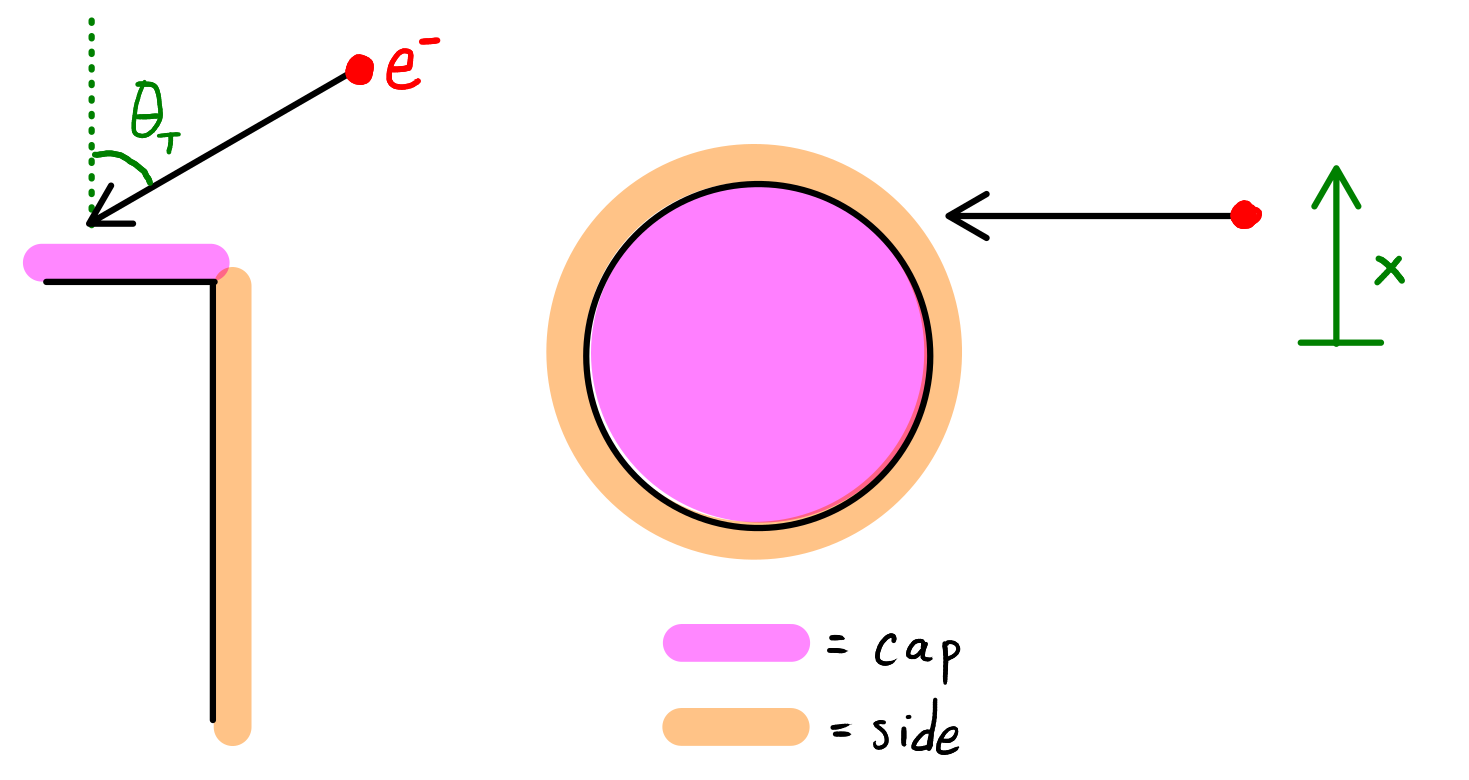
\includegraphics[scale=0.2]{chapter_pa_probe/figures/minimum_velocity_handdrawn.png}
    \caption{Diagram of electron coming from a direction $\theta_T$ and finite impact parameter on the side of the core.}
    \label{fig:pa_minimum_velocity_handdrawn}
\end{figure}

The velocity perpendicular to the cap, $c$, and side, $s$, shown in figure \ref{fig:pa_minimum_velocity_handdrawn} is given by
\begin{align*}
    v_{\perp, c} &= v \cos(\theta_T) \\
    v_{\perp, s} &= v \sin(\theta_T) \sqrt{1 - \frac{x^2}{r^2}}.
\end{align*}
Since the electron needs to overcome the probe potential to be collected, this can be written as
\begin{align*}
    |v_\perp| &\geq v_\perp^\mathrm{min}(x) \\
    \frac{1}{2} m_e v_\perp^\mathrm{min}(x)^2 &= e (V_p - V_0) \\
    \Rightarrow v_{\perp}^\mathrm{min}(x) &= \sqrt{\frac{2e}{m_e} (V_p - V_0)} \\
    \Rightarrow v_{c}^\mathrm{min}(x) &= \frac{1}{\cos{\theta_T}}\sqrt{\frac{2e}{m_e} (V_p - V_0)} \\
    \Rightarrow v_{s}^\mathrm{min}(x) &= \frac{1}{\sin(\theta_T) \sqrt{1 - x^2 / r^2}} \sqrt{\frac{2e}{m_e} (V_p - V_0)}
\end{align*}
where $V_0$ is the plasma potential far from the probe.

% \paragraph{Area}
% \label{spg:pa_area}

\begin{figure}
    \centering
    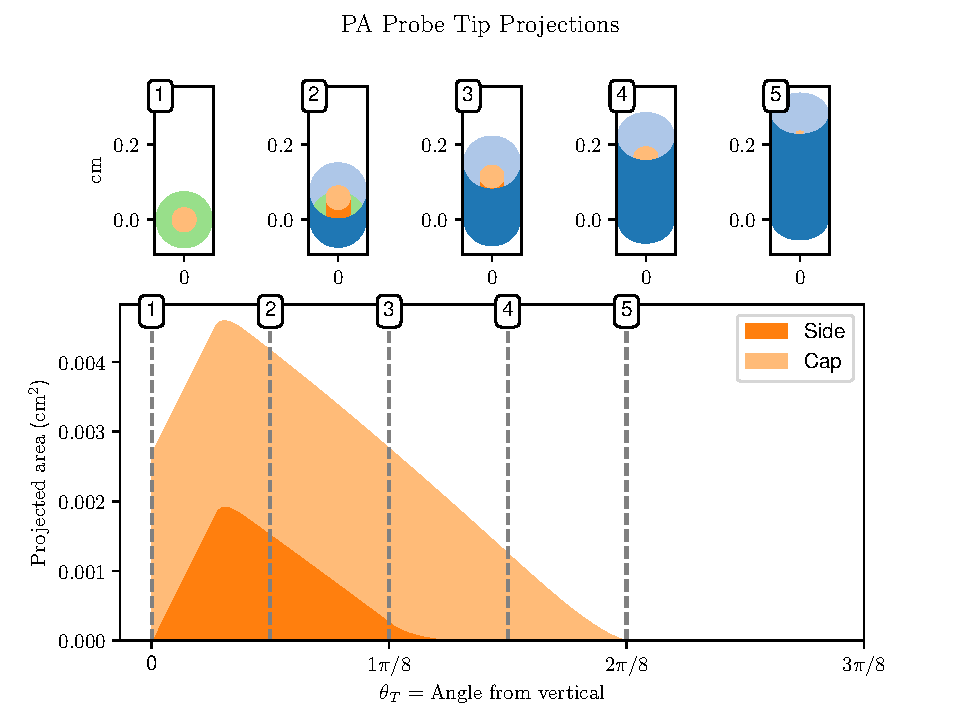
\includegraphics[scale=0.8]{chapter_pa_probe/figures/projected_area.pdf}
    \caption{The bottom plot shows the projected area of the core as a function of direction. The top plots are what the probe tip looks like from specific direction associated with the vertical dashed grey lines. The shell is blue, insulation green, and core orange. The total projected area is maximized near $\pi / 16$ and the largest contributor is the cap.}
    \label{fig:pa_projected_area}
\end{figure}

In the tip oriented coordinate system, we can calculate the area of the cap, $c$, and side, $s$, of the core. We must derive the area projected along some direction since electrons from that direction will only see a limited amount of area. Let $x$ be the horizontal distance from the center of the tip as seen on the x-axis of panels (1)-(5) or figure \ref{fig:pa_projected_area}. The equations for the projected height are
\begin{align*}
    h_{\mathrm{bottom}, s}(x) &= -\cos(\theta_T) \sqrt{r^2 - x^2} \\
    h_{\mathrm{top}, s}(x) &= -\cos(\theta_T) \sqrt{r^2 - x^2} + h \sin(\theta_T) \\
    h_{\mathrm{bottom}, c}(x) &= -\cos(\theta_T) \sqrt{r^2 - x^2} + h \sin(\theta_T) \\
    h_{\mathrm{top}, c}(x) &= \cos(\theta_T) \sqrt{r^2 - x^2} + h \sin(\theta_T) \\
    h_{\mathrm{top}, \mathrm{shell}}(x) &= -\cos(\theta_T) \sqrt{R^2 - x^2} + H \sin(\theta_T)
\end{align*}
where $R$ is the radius of the shell. The constants $h$ and $H$ are the heights of the core and shell respectively measured from the insulation height.

The total exposed height for the side and cap including the covering due to the shell is
\begin{align*}
    h_s(x) &= h_{top,s}(x) - \min\left[h_{top,s}(x), \max\left[h_{bottom,s}(x), h_{top,shell}(x)\right]\right] \\
    h_c(x) &= h_{top,c}(x) - \min\left[h_{top,c}(x), \max\left[h_{bottom,c}(x), h_{top,shell}(x)\right]\right]
\end{align*}

There is a maximum angle at which the side of the core gets fully covered by the shell. There is a larger angle similarly associated with the cap. The conditions of coverage are
\begin{align*}
    h_{\mathrm{top}, \mathrm{shell}}(x = r, \theta_T = \theta_{T,s}^\mathrm{max}) &= h_{\mathrm{top}, s}(x = r, \theta_T = \theta_{T,s}^\mathrm{max}) \quad \mathrm{Side} \\
    \Rightarrow \theta_{T,s}^\mathrm{max} &= \tan^{-1} \left(\frac{\sqrt{R^2 - r^2}}{H - h}\right) \\
    h_{\mathrm{top}, \mathrm{shell}}(x = 0, \theta_T = \theta_{T,c}^\mathrm{max}) &= h_{\mathrm{top}, c}(x = 0, \theta_T = \theta_{T,c}^\mathrm{max}) \quad \mathrm{Cap} \\
    \Rightarrow \theta_{T,c}^\mathrm{max} &= \tan^{-1} \left(\frac{R + r}{H - h}\right).
\end{align*}

% \paragraph{Particle Flux}

We are now ready to calculate the particle flux to the probe. We integrate the distribution function along a specific $\varphi_T$ and $\theta_T$ then integrate over solid angle to calculate the total flux. The particle flux is calculated by multiplying the area along a projected direction by the number of particles from that direction along with the velocity perpendicular to the probe given as
\begin{equation}
    \Gamma_e = \int_{0}^{2\pi}d\varphi_T \sum_{l \in \{s, e\}} \int_{0}^{\theta_{T,l}^{\max}} d\theta_T \int_{-r}^{r} dx \int_{v_{l}^\mathrm{min}(\theta_T, x)}^{\infty}dv \, v^2 \sin(\theta_T) h_l(x) v_{\perp,l} f_e(v, \theta_T, \varphi_T).
    \label{eq:electron_particle_flux}
\end{equation}
$v^2 \sin(\theta_T)$ is due to spherical coordinates, $h_l(x)$ is the height of the projected area going from left to right in the small plots of \ref{fig:pa_projected_area}, the $v_{\perp,l}$ term accounts for the velocity perpendicular to the probe, and $f_e$ is the distribution function.

The particle flux to the side and core for some example plasma parameters and tip directions can be seen in fig \ref{fig:pa_example_particle_flux_to_core}. It can be seen that the flux to the side of the core is very small relative to the cap flux and only starts to become significant near $V_p = 0$. Thus for future analysis and to accelerate the models computational scheme we ignore the side flux.

\begin{figure}
    \centering
    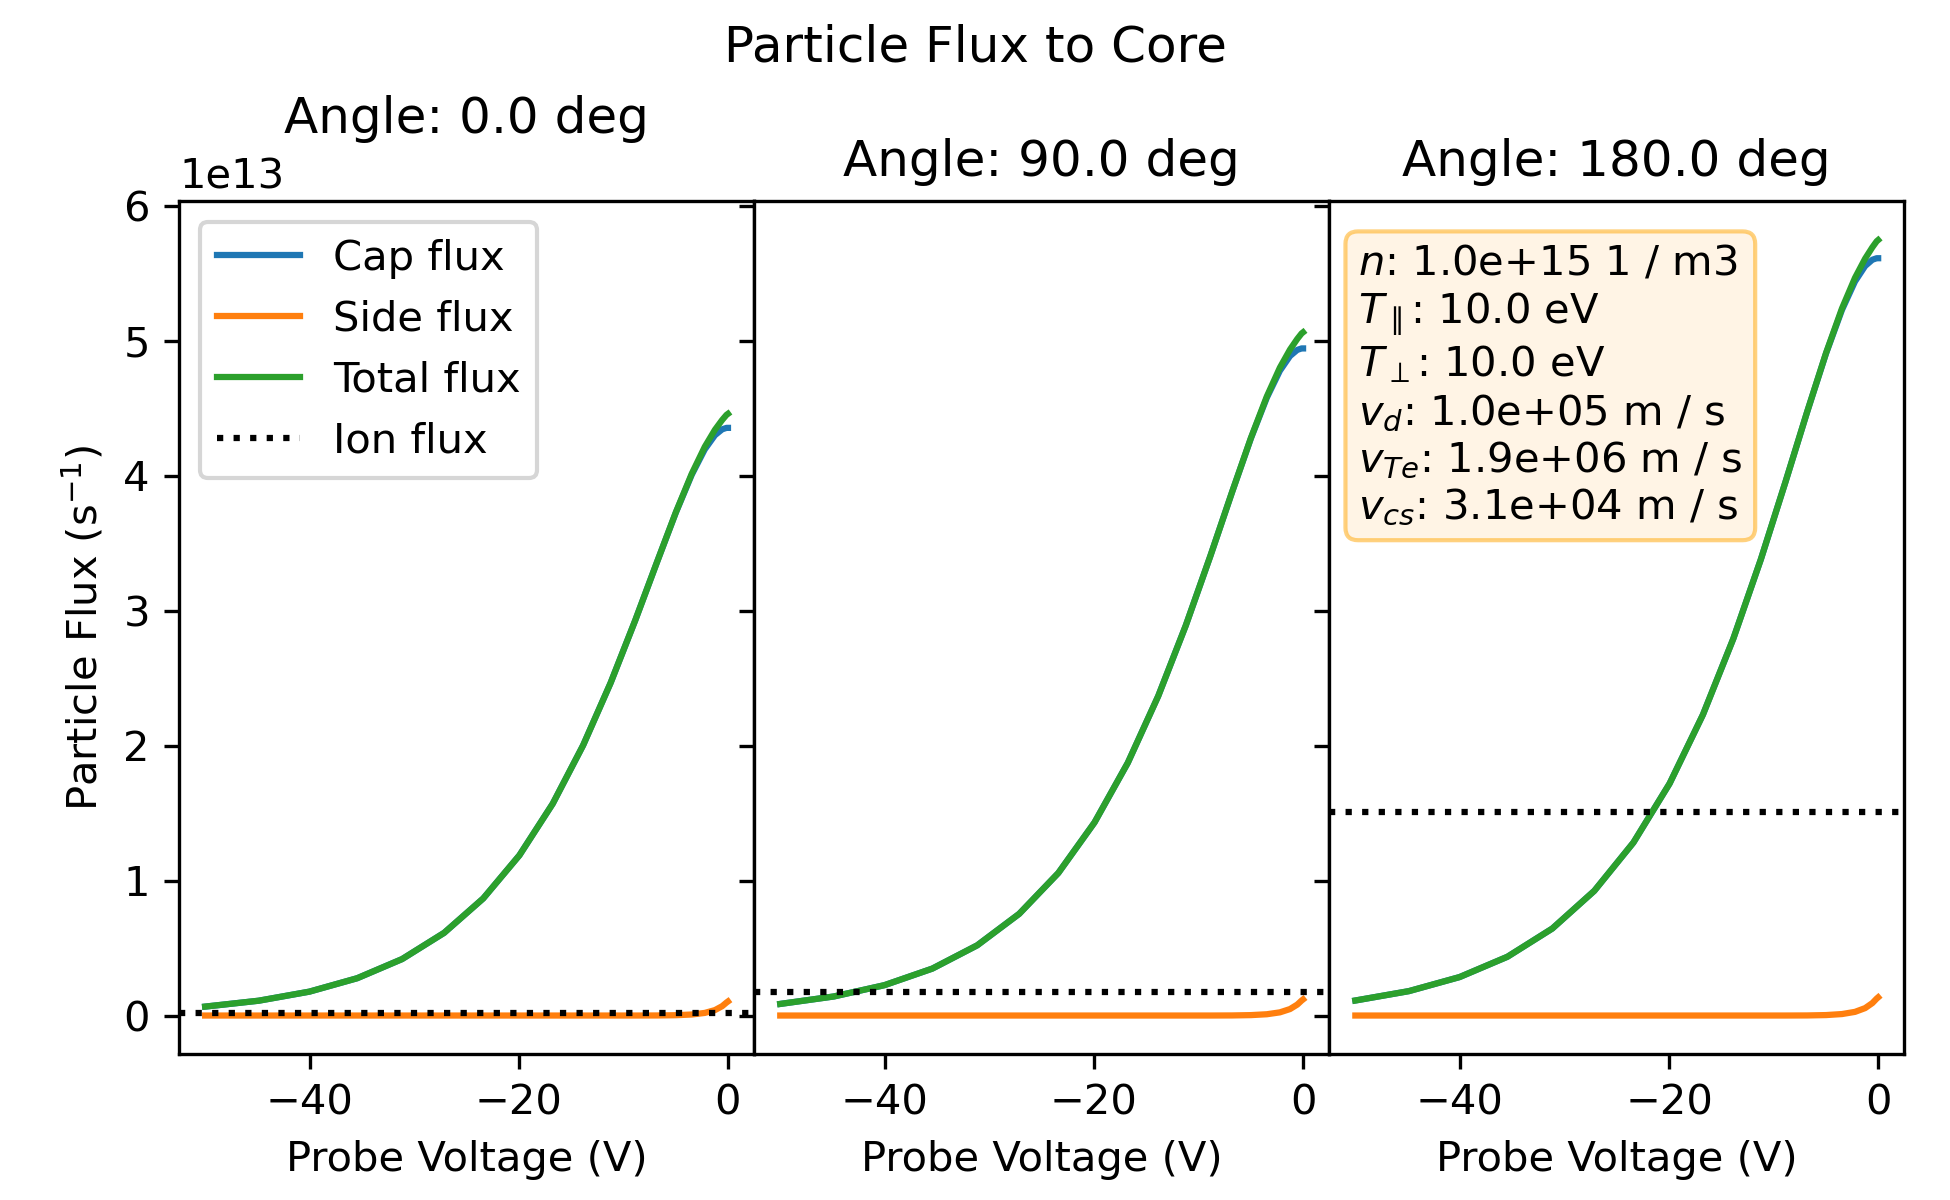
\includegraphics[width=\textwidth]{chapter_pa_probe/figures/example_core_particle_flux.png}
    \caption{Example particle flux to the core for the electrons and ions of a flowing Maxwellian. The ion particle flux is much less for the tip pointed away from the flow (Angle = 0) compared to the tip pointed into the flow (Angle = 180). The electron particle flux is much less affected by the flow but does change some in magnitude. The particle flux to the side of the tip is very small in comparison to the flux to the cap. Plasma parameters are given in the legend with $v_d \coloneq$ drift velocity, $v_{Te} \coloneq$ thermal speed, and $v_{cs} \coloneq$ sound speed.}
    \label{fig:pa_example_particle_flux_to_core}
\end{figure}

% \subsubsection{Theoretical JV curves}

Now that we have developed a theory for the expected current to a probe given some plasma parameters, we simulate the expected IV-characteristics the probe should see.

% \paragraph{Reading radar plots}

% Normally, IV-characteristics are read using a 2D plot of the probe potential vs. probe current (or current density). As we want to incorporate a directional aspect to this plot let's use a radar plot.

% \subparagraph{Radar axis}

% The radar plot has a direction component which is the angle around the circle. For the probe potential we use the radial distance and choose a minimum voltage to be at zero radius (not plotting any points with bias less that the minimum voltage). The color is then the current to the probe at a given angle and voltage. We also draw a grey line where the floating potential is (i.e. there is no current to the probe).

% \paragraph{Solutions}
Figure \ref{fig:pa_theoretical_radar_plots} shows some example electron distribution functions (top row) and their corresponding IV-characteristic radar plots (bottom row). In a Maxwellian plasma with no drift (left column) the IV radar plot looks the same for any angle. This is expected since the plasma has no directional dependence. Once we add a drift, middle column, the distribution changes shape. In this case the plasma is flowing upward with a drift velocity that is small relative to the electron thermal speed but is on the order of tenths of ion sound speed. This means that the Mach effect will come into play which leads to more ion current hitting probes pointing into the flow (pointing downwards) and very little ion current for probes pointed in the direction of flow. Finally, a drifting bi-Maxwellian will have both a Mach effect and a difference in temperature. Here we've set the drift to be upwards and the magnetic field direction (parallel direction) to be up and to the left. When this is the case we have two noticeable features. Ion current has a directional dependence due to the drift and the electron current to the probe is much higher in the direction of higher temperature than in the direction of low temperature. This is as to be expected because there is higher electron flux in the high electron temperature direction.

\begin{figure}
    \centering
    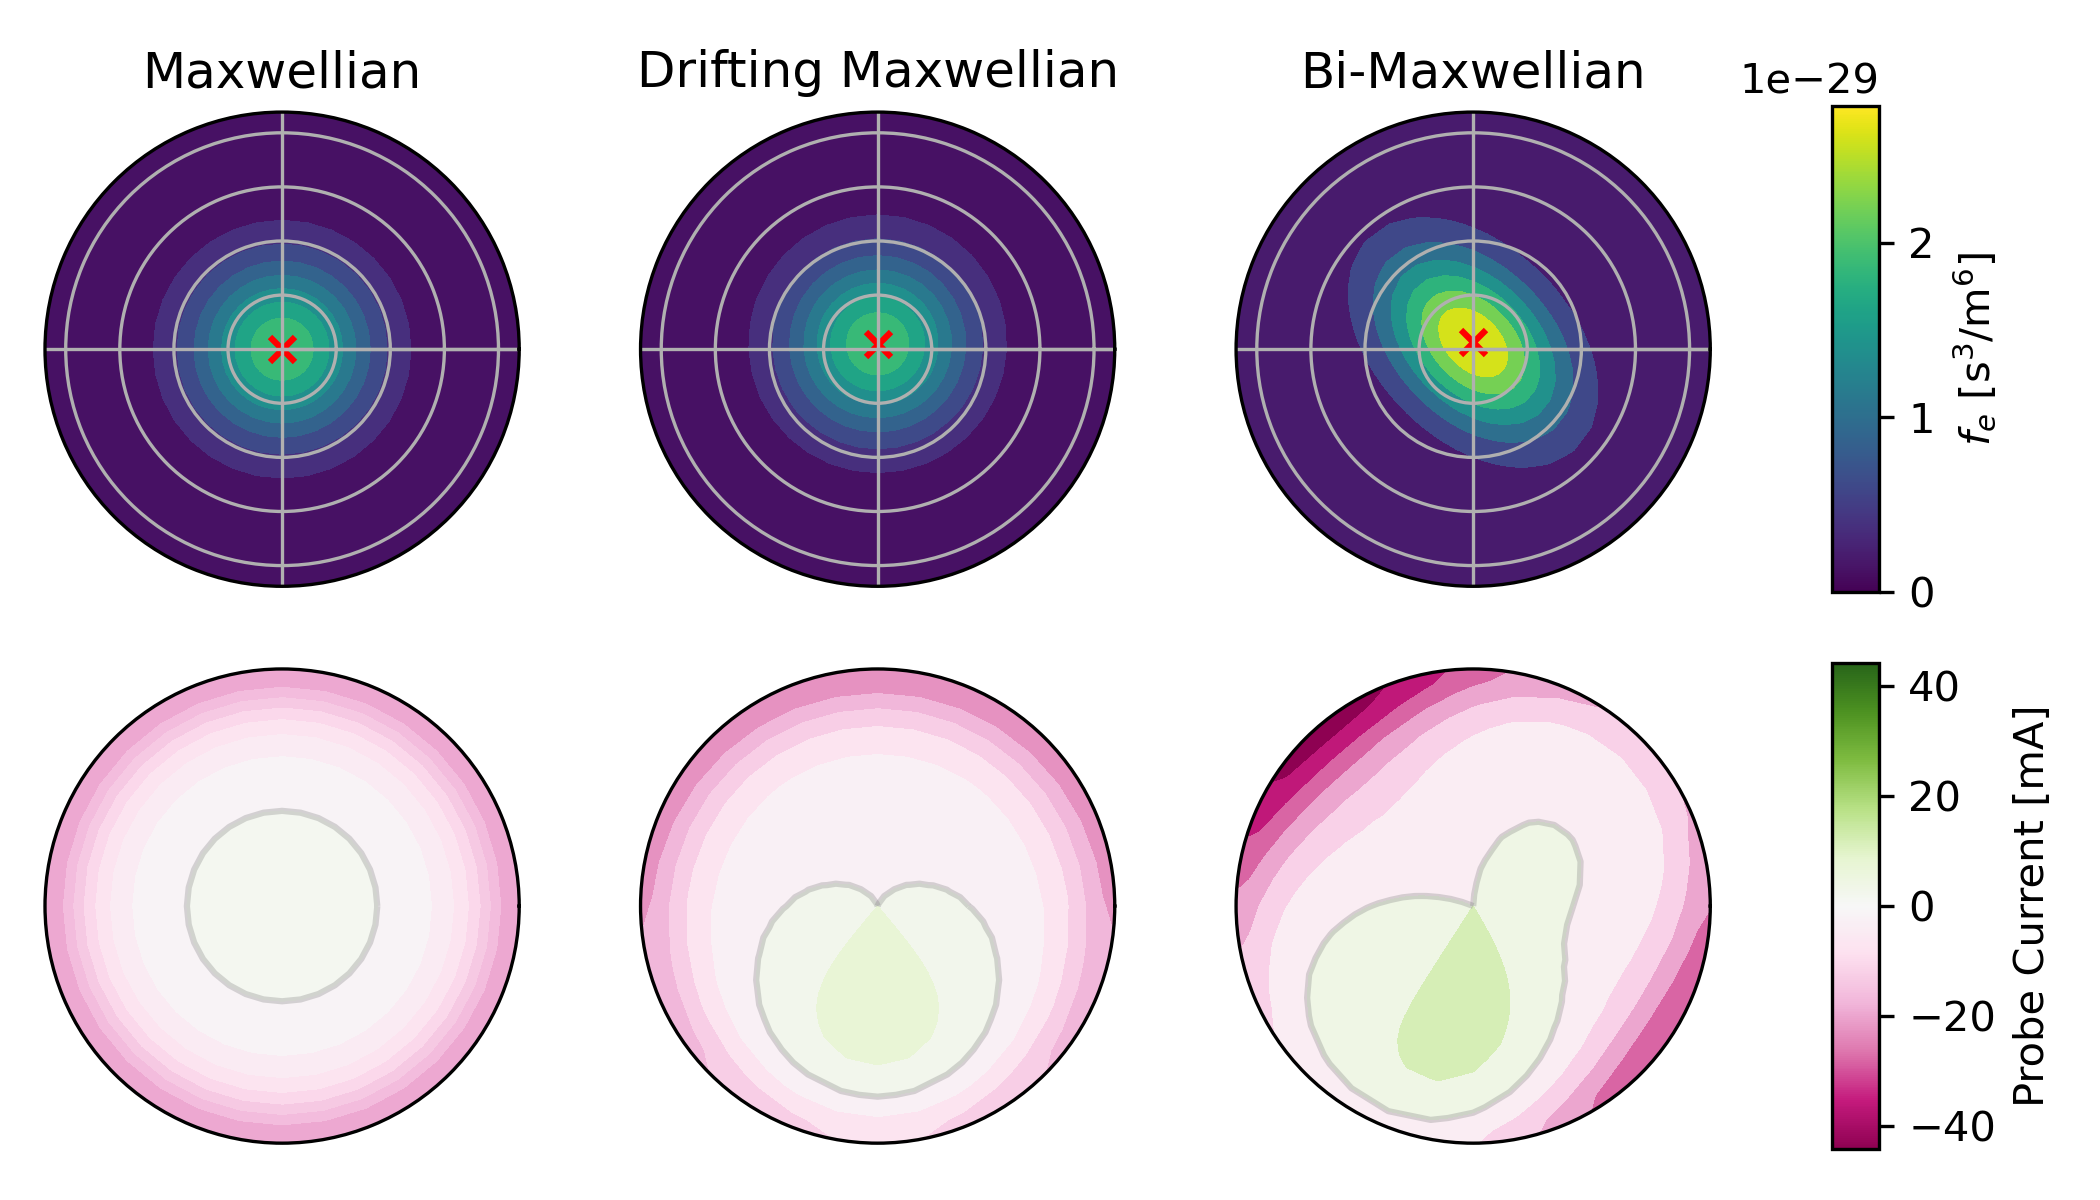
\includegraphics[width=\textwidth]{chapter_pa_probe/figures/theoretical_pa_radar_plots.png}
    \caption[Theoretical plasma distributions and IV-characteristics]{This figure shows three possible electron distribution functions in the top row and their corresponding IV-characteristics in the bottom row. For the distribution functions, the angle is the direction of the velocity, the radius is the velocity magnitude, and the color is the phase space density. The IV-characteristics show the direction of the tip as angle, the probe potential as radius, and the expected current to the probe as color. The grey contour is identifies the probe potential at which the current to the probe is zero.}
    \label{fig:pa_theoretical_radar_plots}
\end{figure}

\subsection{Individual Tip Model}
\label{sss:pa_individual_tip_fitting}

Instead of fitting all the tips at once, we can instead fit each using a routine similar to that for the multi-tip Langmuir probe and then combine the individual plasma parameters from each tip into bulk properties.

% \subsubsection{Why do this instead}

We have found that the full model suffers from optimization difficulties. It is computationally intensive to recalculate the IV-characteristic when optimizing the parameters and suffers from fitting too many parameters, namely the electron density, parallel temperature, perpendicular temperature, and three components of the drift velocity. We find that this algorithm faces some difficulty in correctly reproducing the characteristic magnitudes which may be due to non-Maxwellian features in the plasma and the simplicity of this model not correctly reproducing the actual plasma response to an acceptable degree.

% \subsubsection{Individual Tip Theories}

% Let's take a look as to the options we have available for fitting each tip separately.

% \paragraph{Multi-tip methods}

In sections \ref{sss:multitip_hutchinson_theory} and \ref{sss:multitip_brl_theory} we discussed two plasma theories to predict the expected current to a simple Langmuir probe given a set of plasma parameters describing an unmagnetized Maxwellian plasma. Both of these methods, and many other Langmuir probe theories, show the same general trends for the expected current to a Langmuir probe independent of theory approximations and magnetization. Thus we can apply each of these theories to each tip and fit the plasma parameters using Orthogonal Distance Regression.

% \paragraph{Exponential}
% \label{spg:pa_theory_exponential}

While both of the previous theories, Hutchinson and BRL, work well for a normal Langmuir probe, we find that the geometry of our system may lead to different ratios of the electron to ion current than expected from one of these physically derived theories.

% \subparagraph{Ions don't hit core}


\begin{figure}
    \centering
    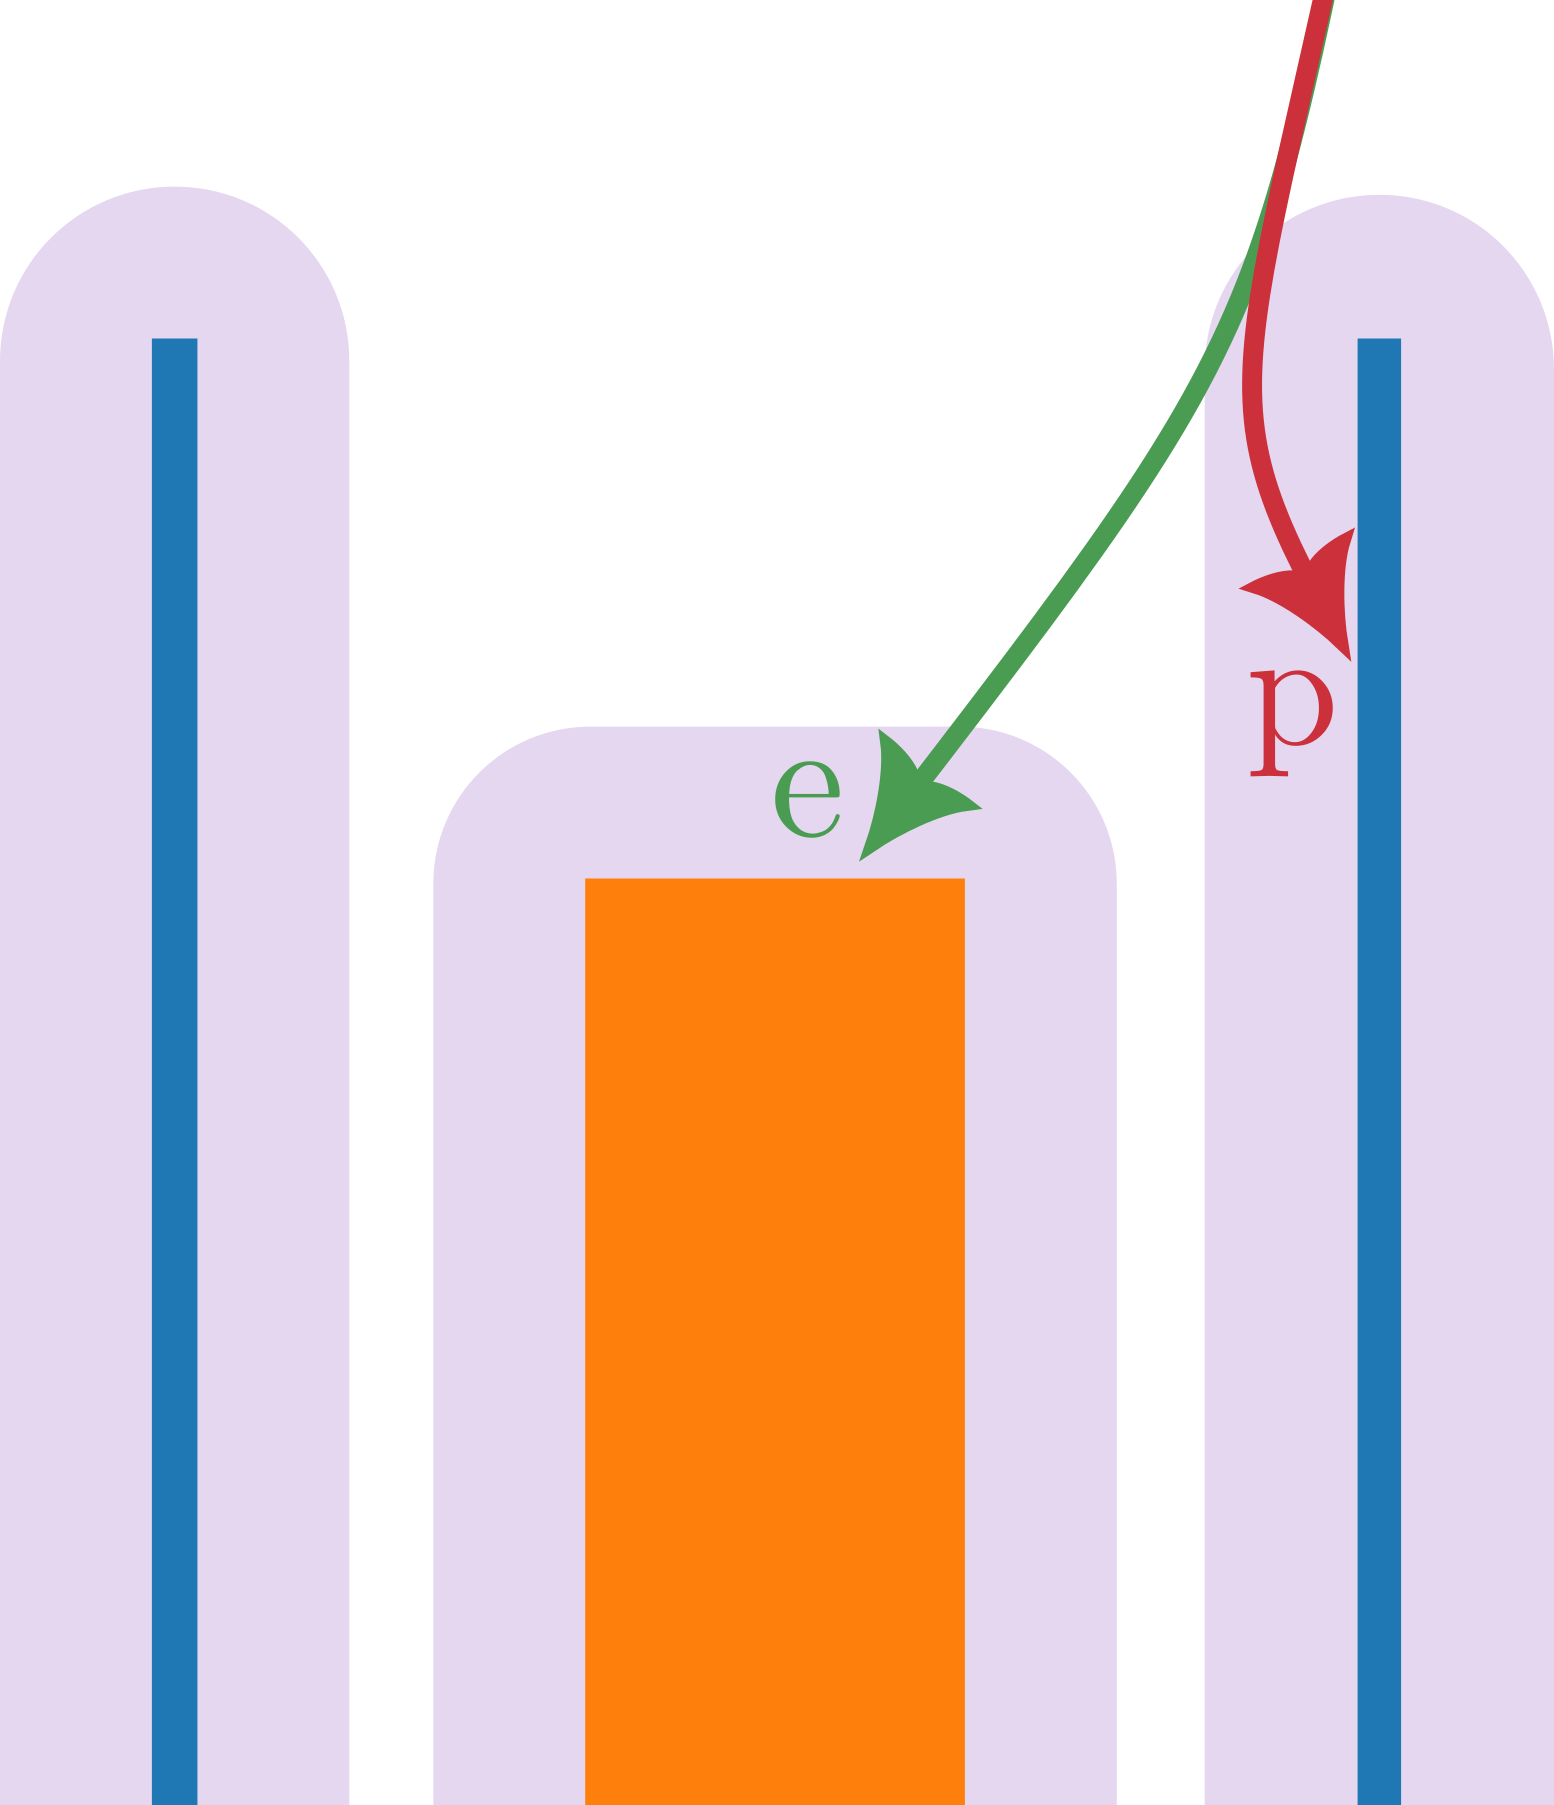
\includegraphics{chapter_pa_probe/figures/pa_ion_attraction.png}
    \caption[PA Ion vs. Electron trajectories]{This figure shows some what may occur to ions in comparison to electrons when the probe is attracting ions. Ions, in this case protons signified by `p' in red, are attracted to the probe and when passing close to the shell on their way to the core they hit the shell. The electrons (green, e) are instead repelled from the shell (blue rectangles) and focused toward the core (orange rectangle). The purple regions are the extent of the sheath over which there is a non-negligible electric field pointed toward the conductors.}
    \label{fig:pa_ion_vs_electron_trajectories}
\end{figure}

% \subparagraph{More Free Parameters}

As already noted, the current to a Langmuir probe is well approximated by a constant ion current and an exponential electron current like as seen in Hutchinson's model.
Figure \ref{fig:pa_ion_vs_electron_trajectories} shows an approximate sheath around the core (orange rectangle) and shell (blue rectangles) as a cross section of the probe tip. Since ions will be consumed by the shell and electrons will be focused towards the core, the expected ratio of ion versus electron current will be smaller than expected from a simple Langmuir probe theory. Thus in fitting the IV-characteristics from each tip we will fit the electron and ion densitiies separately.

% \subparagraph{Model equation}

To simplify fitting, we've taken the current to the tip to be
\begin{equation}
    I_p(V_p) = -A \exp(V_p / B) + C
    \label{eq:pa_exp_model}
\end{equation}
where the parameters to fit ($A$, $B$, and $C$) are greater than zero.

% \subparagraph{Plasma parameters to exponential parameters}

Using Hutchinson's model, equation \ref{eq:multitip_hutchinson_model}, we can write the terms in the exponential model, eq. \ref{eq:pa_exp_model}, as
\begin{align}
    A(n_e, T_e; V_\text{plasma}) &= n_e e \sqrt{\frac{e T_e}{m_i}} \left[\frac{1}{2} \sqrt{\frac{2 m_i}{\pi m_e}} \exp\left(\frac{- V_\text{plasma}}{T_e}\right)\right] \label{eq:pa_plasma_to_exp_params_A}\\
    B(T_e) &= T_e \\
    C(n_i, T_e; V_\text{plasma}) &= n_i e \sqrt{\frac{e T_e}{m_i}} \exp\left(-\frac{1}{2}\right).
\end{align}

% \subparagraph{Exponential parameters to plasma parameters}

Since we have four plasma parameters and three exponential parameters, we can't invert the entire fitting procedure. To correct for this, we use the shell's measured plasma potential to remove one parameter. Thus we have
\begin{align}
    n_e(A, B) &= \left. A \middle/ e \sqrt{\frac{e B}{m_i}} \left[\frac{1}{2} \sqrt{\frac{2 m_i}{\pi m_e}} \exp\left(\frac{- V_\text{plasma}}{B}\right)\right] \right. \\
    T_e(B) &= B \\
    n_i(C, B) &= \left. C \middle/ e \sqrt{\frac{e B}{m_i}} \exp\left(-\frac{1}{2}\right) \right.
\end{align}
where everything on the right side is an external input or a fit parameter.

% \subparagraph{Converting fit errors}

After fitting the exponential parameters, our fitting routine returns a set of standard deviations for each fit parameter. Assuming linear error propagation, the standard deviations for each of the plasma parameters are
\begin{align}
    \sigma_{ne} &= \sqrt{(\partial_A n_e(A, B) \sigma_A)^2 + (\partial_B n_e(A, B) \sigma_B)^2} \nonumber \\
    &= \sqrt{\frac{\pi}{2}} \sqrt{\exp\left(\frac{2 V_\text{plasma}}{B}\right) \frac{m_e}{B^5 e^3} \left(4 B^4 \sigma_A^2 + A^2 \sigma_B^2 (B + 2 V_\text{plasma})\right)} \\
    \sigma_{Te} &= \sigma_B \\
    \sigma_{ni} &= \sqrt{(\partial_C n_e(C, B) \sigma_C)^2 + (\partial_B n_e(C, B) \sigma_B)^2} \nonumber \\
    &= \frac{\exp\left(\frac{1}{2}\right)}{2}\sqrt{\frac{m_i}{B^3 e^3} \left(C^2 \sigma_B^2 + 4 B^2 \sigma_C^2\right)}.
\end{align}

% \subsubsection{Extracting plasma parameters}

We have derived a model for each tips IV-characteristics and will now describe a method for calculating bulk plasma properties using spherical harmonics.

% \paragraph{Spherical harmonics}

We align the spherical harmonic's coordinate system with the local magnetic field direction. By using spherical harmonics that only vary as a function of polar angle, $\theta$, we can measure the dependence on angle ignoring agyrotropic effects.

% \subparagraph{Parallel and Perpendicular Temperature}

If we ignore the drift velocity in the distribution function (since drifts in our experiment are small relative to the electron thermal speed), equation \ref{eq:drifting_bimaxwellian}, we find that the term in the exponential coefficient takes the form
\begin{equation}
    -\frac{e m_e}{2} v^2 \left(\frac{\cos^2\theta}{T_\parallel} + \frac{\sin^2\theta}{T_\perp}\right)
\end{equation}
where $\theta$ is the angle between the magnetic field and the velocity (whose magnitude is given by $v$). Thus we can write a directional temperature as
\begin{equation}
    T(\theta) = \frac{T_\perp T_\parallel}{T_\parallel \sin^2 \theta + T_\perp \cos^2 \theta}.
    \label{eq:pa_directional_temperature}
\end{equation}
This can not be written in a finite number of spherical harmonics but the inverse temperature can be written as
\begin{align}
    \frac{1}{T(\theta)} &= \frac{T_\parallel \sin^2 \theta + T_\perp \cos^2 \theta}{T_\perp T_\parallel} \\
    &= \frac{T_\parallel}{T_\perp T_\parallel} + \frac{T_\perp - T_\parallel}{T_\perp T_\parallel} \cos^2\theta \\
    &= \frac{2 \sqrt{\pi}}{3} \left(\frac{2 T_\parallel + T_\perp}{T_\parallel T_\perp} Y_{0,0}(\theta, \phi) - \frac{2}{\sqrt{5}} \frac{T_\parallel - T_\perp}{T_\parallel T_\perp} Y_{2, 0}(\theta, \phi)\right) \label{eq:pa_bimax_inv_temp}
\end{align}
where $Y_{i,j}$ are the spherical harmonics.

Now, the mean temperature of all the tips is not necessarily the mean temperature calculated from the second moment of the distribution function. From the distribution function integration, the mean temperature is
\begin{equation}
    \frac{1}{2} m_e \iiint v^2 f(v) \, \dd \vb{v} = \frac{T_\parallel + 2 T_\perp}{3}.
\end{equation}
If we assume that each tip only measures the distribution function along a ray in the direction of the tip then we need to average the directional temperature, equation \ref{eq:pa_directional_temperature}. As we are really fitting $1/T$ we find that
\begin{equation}
    T_\text{avg} = \left(\frac{\iint 1 / T(\theta) \, \dd \Omega}{\iint \, \dd \Omega}\right)^{-1} = \frac{3 T_\parallel T_\perp}{2 T_\parallel + T_\perp}.
\end{equation}
To note, if we were to instead average the temperature, not the inverse temperature, we would find
\begin{equation}
    T_\text{avg,non-inverse} = \begin{cases*}
        \frac{T_\parallel T_\perp}{\sqrt{T_\parallel \left(T_\perp - T_\parallel \right)}} \cos^{-1}\left(\sqrt{\frac{T_\parallel }{T_\perp }}\right) & if $T_\parallel < T_\perp$  \\
        \frac{T_\parallel T_\perp}{\sqrt{T_\parallel \left(T_\parallel - T_\perp \right)}} \cosh^{-1}\left(\sqrt{\frac{T_\parallel }{T_\perp }}\right) & if $T_\parallel > T_\perp$
    \end{cases*}
\end{equation}
which is larger than $T_\text{avg}$ for all $T_\parallel / T_\perp$. The differences between averaging schemes can be seen in figure \ref{fig:pa_t_averaging}.

\begin{figure}
    \centering
    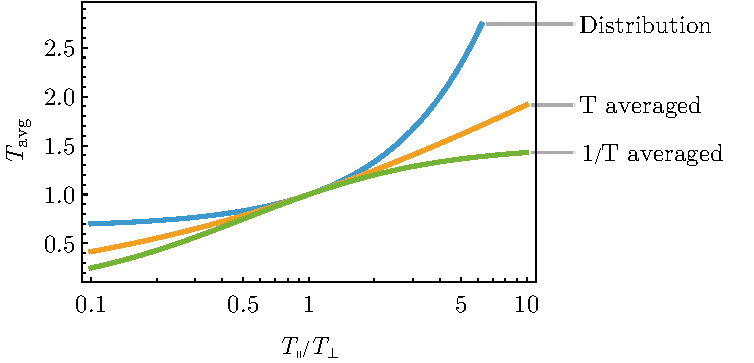
\includegraphics{chapter_pa_probe/figures/t_averaging_comparison.pdf}
    \caption[T averaging methods]{A comparison of the various methods for averaging the temperature. Averaging the distribution always leads to the largest average temperature whereas averaging the temperature by direction scales at a different rate.}
    \label{fig:pa_t_averaging}
\end{figure}

% \subparagraph{Tri-Maxwellian Temperature}

In calculating the parallel and perpendicular temperature we enforced that temperatures of the distribution had to be in the coordinate system of the local magnetic field direction. This forces us to only be able to see temperature differences aligned with the field and thus may introduce some errors into our analysis. Additionally, we would like to identify if the distribution is actually rotating with the magnetic field as expected.

We can relax this constraint by considering a tri-Maxwellian distribution given by
\begin{equation}
    f(\vb{v}) \propto \exp\left(-\frac{(\vb{v}\cdot\hat{t}_1)^2}{T_1} -\frac{(\vb{v}\cdot\hat{t}_2)^2}{T_2} -\frac{(\vb{v}\cdot(\hat{t}_1 \cross \hat{t}_2))^2}{T_3}\right)
\end{equation}
where $\hat{t}_1$, $\hat{t}_2$, and $\hat{t}_3$ are orthonormal and aligned with $T_1$, $T_2$, and $T_3$ respectively. If we define a spherical coordinate system with $\hat{t}_1$ as the polar axis we can then write
\begin{equation}
    \frac{1}{T_\text{tri}(\theta', \phi')} = \frac{\cos^2\theta'}{T_1} + \frac{\sin^2\theta'\cos^2\phi'}{T_2} + \frac{\sin^2\theta'\sin^2\phi'}{T_3}.
    \label{eq:pa_trimax_inv_temp}
\end{equation}
We leave it as an exercise to the reader to show that this reproduces the bi-Maxwellian inverse temperature equation, eq. \ref{eq:pa_bimax_inv_temp}.

Let the unprimed coordinates $\theta$ and $\phi$ represent the angles relative to whatever set of axis are convenient for calculating spherical harmonics (not necessarily aligned with the temperatures). We can construct a tensor from this inverse temperature equation by populating each element in the matrix, $T$, via
\begin{align*}
    T_{ij} &= \int x_i x_j \frac{1}{T(\theta, \phi)} \dd \Omega \\
    &= c_{0,0} y_{0,0} + \sum_{m=-2}^2 c_{2,m}^{ij} y_{2,m}
\end{align*}
where
\begin{align*}
    c_{l,m}^{ij} &= \int x_i x_j Y_{l,m}(\theta, \phi) \dd \Omega \\
    y_{l,m} &= \int \frac{1}{T(\theta, \phi)} Y_{l,m}(\theta, \phi) \dd \Omega.
\end{align*}

Now we diagonalize this tensor into $T = P D P^{-1}$ where this acts to rotate this arbitrarily directed tri-Maxwellian into a coordinate system aligned with $\hat{t}_1$, $\hat{t}_2$, and $\hat{t}_3$. The eigenvectors contained in $P$ give the directions of each temperature and the eigenvalues $\lambda_i$, which make up the diagonal of $D$, are just $T_{ij}'$ (the elements of $T$ in the coordinate system aligned with the temperatures).

Thus we can solve for $y_{l,m}'$ in our rotated coordinate system by solving
\begin{align}
    \begin{bmatrix}
        \lambda_1 \\
        \lambda_2 \\
        \lambda_3
    \end{bmatrix} = \begin{bmatrix}
        c_{0,0} & c_{2,0}^{xx} & c_{2,\pm 2}^{xx} \\
        c_{0,0} & c_{2,0}^{yy} & c_{2,\pm 2}^{yy} \\
        c_{0,0} & c_{2,0}^{zz} & c_{2,\pm 2}^{zz} \\
    \end{bmatrix} \begin{bmatrix}
        y_{0,0}' \\
        y_{2,0}' \\
        y_{2,+2}' + y_{2,-2}'
    \end{bmatrix}.
\end{align}
Note that $c_{2,+2} = c_{2,-2}$ so we've combined those spherical harmonics.

Returning to our inverse temperature equation, \ref{eq:pa_trimax_inv_temp}, we can split the inverse temperature into spherical harmonics as
\begin{align*}
    \frac{1}{T_\text{tri}(\theta', \phi')} =& y_{0,0}' Y_{0,0}(\theta', \phi') + y_{2,0}' Y_{2,0}(\theta', \phi') \\
    &+ (y_{2,+2}' + y_{2,-2}') \left(Y_{2,+2}(\theta', \phi') + Y_{2,-2}(\theta', \phi')\right) \\
    y_{0,0}' =& \frac{2\sqrt{\pi}}{3} \frac{T_1 (T_2 + T_3) + T_2 T_3}{T_1 T_2 T_3} \\
    y_{2,0}' =& -\frac{2}{3} \sqrt{\frac{\pi}{5}} \frac{T_1 (T_2 + T_3) - 2 T_2 T_3}{T_1 T_2 T_3} \\
    y_{2,+2}' + y_{2,-2}' =& -\sqrt{\frac{8 \pi}{15}} \frac{T_2 - T_3}{T_2 T_3}.
\end{align*}
These equations can be solved for the temperatures which along with the eigenvectors gives us the tri-Maxwellian temperatures and directions.


% \subparagraph{Ion Drift Velocity}

From equation \ref{eq:pa_ion_current_density_full} we can see that the logarithm of the ion current density can be decomposed into a finite number of spherical harmonics and thus we can measure the ion drift velocity. We already fit $n_i$, which in our simple model is proportional to the ion current density. The logarithm of the current density is
\begin{align}
    \ln(J_i(v_f, \theta')) =& \ln\left(e n_i \sqrt{\frac{e T_e}{m_i}} \Gamma_0\right) \nonumber \\
    &+ \left\{\frac{1}{2} v_f \sqrt{\frac{m_i}{e T_e}} \left[(1 - \cos \theta') K_u - (1 + \cos \theta') K_d\right]\right\}.
    \label{eq:pa_log_ion_current_density}
\end{align}
$\theta'$ is the angle between the flow direction, $(\theta_f, \phi_f)$, and the tip direction, $(\theta_t, \phi_t)$ which can be written as
\begin{align*}
    \theta' = \cos^{-1}(&\left(\sin\theta_t \cos\phi_t \hat{x} + \sin\theta_t \sin\phi_t \hat{y} + \cos\theta_t \hat{z}\right) \cdot \\
    &\left(\sin\theta_f \cos\phi_f \hat{x} + \sin\theta_f \sin\phi_f \hat{y} + \cos\theta_f \hat{z}\right)).
\end{align*}
As the ion density is a real number, we use spherical harmonics defined in the real domain:
\begin{equation*}
    Y_{l,m}(\theta, \phi) = \begin{cases*}
        \frac{i}{\sqrt{2}} \left(Y_l^m(\theta, \phi) - (-1)^m Y_l^{-m}(\theta, \phi)\right) & if $m < 0$\\
        Y_l^0(\theta, \phi) & if $m = 0$\\
        \frac{1}{\sqrt{2}} \left(Y_l^{-m}(\theta, \phi) + (-1)^m Y_l^{m}(\theta, \phi)\right) & if $m > 0$
    \end{cases*}.
\end{equation*}
To note, for the case of extracting the parallel and perpendicular temperature there was no azimuthal dependence on $Y_{0,0}$ and $Y_{2,0}$ so we did not have to convert the harmonic to real space.

We can then write the spherical harmonic coefficients of equation \ref{eq:pa_log_ion_current_density}:
\begin{align*}
    c_{0,0} &= \sqrt{\pi} \left((K_u - K_d) \sqrt{\frac{m_i}{e T_e}} v_f + 2 \ln\left(e n_i \sqrt{\frac{e T_e}{m_i}} \Gamma_0\right)\right) \\
    c_{1,-1} &= -(K_u + K_d) \sqrt{\frac{\pi}{3}}\sqrt{\frac{m_i}{e T_e}} v_f \sin \theta_f \sin \phi_f \\
    c_{1,0} &= -(K_u + K_d) \sqrt{\frac{\pi}{3}}\sqrt{\frac{m_i}{e T_e}} v_f \cos \theta_f \\
    c_{1,+1} &= -(K_u + K_d) \sqrt{\frac{\pi}{3}}\sqrt{\frac{m_i}{e T_e}} v_f \sin \theta_f \cos \phi_f
\end{align*}
We can see that $c_{1,-1}$, $c_{1,0}$, and $c_{1,+1}$ recover the flow velocity vector given the electron temperature. $c_{0,0}$ sets the ion number density once we calculate the flow velocity magnitude. It can be seen that $c_{1,-1}$, $c_{1,0}$, and $c_{1,+1}$ construct a vector antiparallel to the flow such that
\begin{equation*}
    c_{1,+1} \hat{x} + c_{1,-1} \hat{y} + c_{1,0} \hat{z} = -(K_u + K_d) \sqrt{\frac{\pi}{3}}\sqrt{\frac{m_i}{e T_e}} \vb{v}_f.
\end{equation*}

% \paragraph{Error bars}

In calculating the error on the drifts or temperatures, we use a Monte-carlo method of the following form. For calculating the drift we are taking spherical harmonics of the ion density. From the individual tip fits we get $n_i^j \pm \sigma_{ni}^j$. Thus we can sample that distribution and recalculate the drift velocity many times. This then gives us a distribution of drift velocities for a single time point that let us derive error bars on the drift velocity. The same can be done for the temperatures where we recalculate the spherical harmonic coefficients many times for distributions of temperature measurements.

\section{Curve Fitting}

To measure the plasma parameters we first cleanup the data by combining multiple shots and then use data from both the shell and core to get the final plasma parameters of interest.

\subsection{Combining multiple shots}

Over many distinct shots, we sample the IV-characteristic such that we can well fit the resulting plasma parameters. To do so, we take shots at a variety of different bias voltages and with the core current paths un-swapped and swapped. In total, this requires on the order of 100 shots and thus we must remove outlier shots and align each shot in time.

% \subsubsection{Timing alignment}
% \label{ss2:pa_timing_alignment}

\begin{figure}
  \centering
  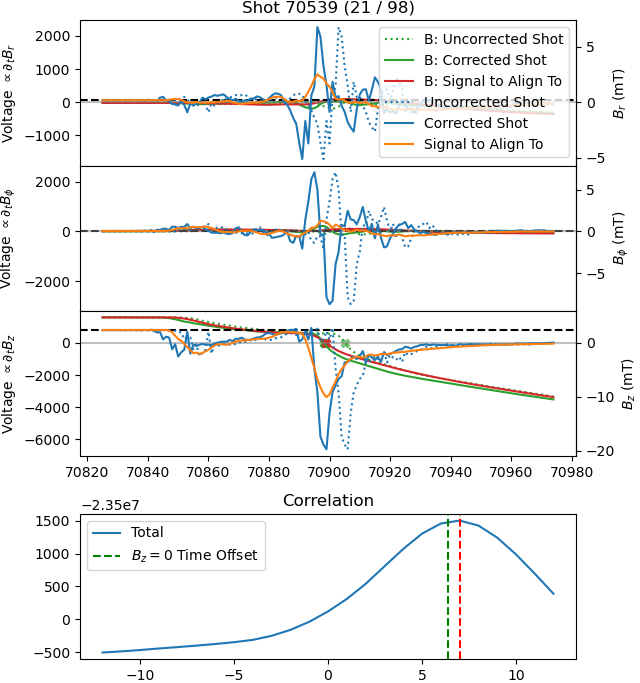
\includegraphics[width=\textwidth]{chapter_pa_probe/figures/PA_example_time_alignment.png}
  \caption{The alignment procedure for a single shot. Alignment can occur in one of two ways. Either the cross-correlation of the B-dot signals can be maximized or the crossing time of $B_z = 0$ can be aligned. Here we've chosen a particularly egregious shot for alignment purposes since the alignment process offsets the arrays by 8 time samples for the B-dot cross-correlation (0.8 \textmu s) or 7 time samples for the $B_z = 0$ alignment (red and green dashed lines respectively in bottom panel). The top three panels show the unaligned data from the shot (blue dotted for both B-dot and B). The orange and red lines are the data to align with which is found using the mean of the B-dot and B signals for all of the shots. The x's in the $\partial_t B_z$ panel are where $B_z = 0$ for the unaligned and aligned data.}
  \label{fig:pa_example_time_alignment}
\end{figure}

\begin{figure}
  \centering
  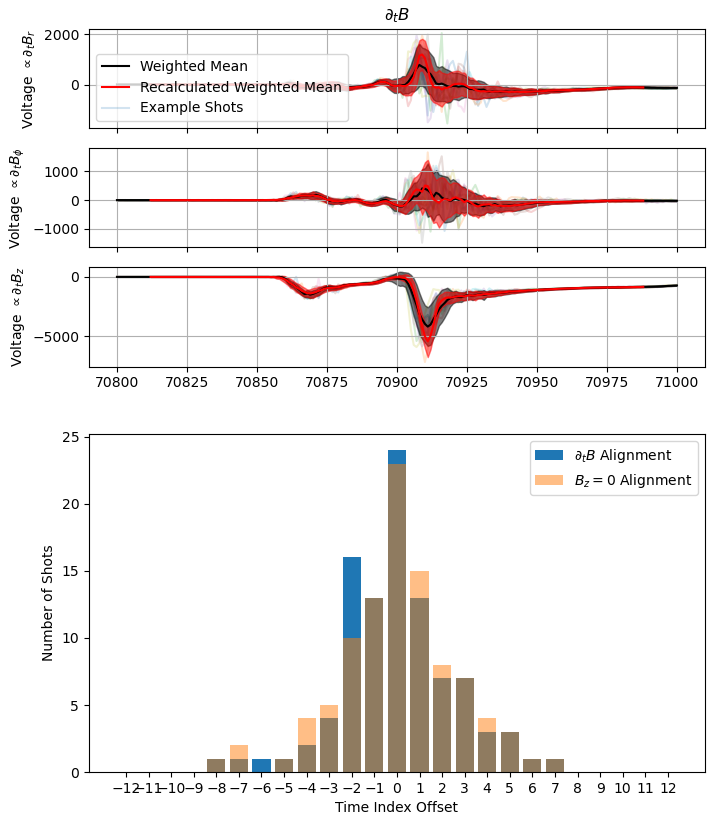
\includegraphics[width=\textwidth]{chapter_pa_probe/figures/PA_time_alignment_over_many_shots.png}
  \caption{An example of the effects of aligning data for the PA probe. Using 98 shots we have aligned the data in time using either cross-correlation of the B-dot signals on the probe or by aligning the $B_z = 0$ crossing time index. The differences in the alignment method are seen in the bottom figure. The histograms for both methods are similar and thus give similar alignment results. The top three panels show example B-dot traces (light colored lines). The average of all 98 signals before alignment is seen in black with one standard deviation bounds. After alignment, a new mean is calculated and shown in red. It can be seen that the standard deviation is far smaller after alignment and the red mean has less smoothed features.}
  \label{fig:pa_time_alignment_many_shots}
\end{figure}

Since each shot is slightly different, we adjust the time index for each shot such that the features in the magnetic field data align. An example of this can be seen in Fig. \ref{fig:pa_example_time_alignment} where the actual shot timing is eight time samples (0.8 \textmu s) after the normal shot timing. We can correct this in one of two ways:

\paragraph{B-dot cross-correlation}

Cross-correlation is a method of finding when different signals align by applying different amounts of offset between the two signals and calculating
\begin{equation}
    C_{i,j}(\Delta t) = \frac{1}{T_i T_j} \int \vb{S}_i(t) \cdot \vb{S}_j(t + \Delta t) \, \dd t.
\end{equation}
Both of our signals are of the same length but because we are shifting them by $\Delta t$ the amount of time they overlap goes as $T_i = T - \Delta t$. Additionally as we have a discrete set of sample points, this is a sum in our case and subtracting off the mean of both signals before multiplying them (i.e. $\vb{S} \rightarrow \vb{S} - \overline{S}$) helps with correlation.

If we take the cross-correlation of the probe B-dot signals in machine coordinates we can maximize that to find when the signals for that shot best align with the average shot.

During the initial phase when the capacitor bank trigger activates and later, when the bank switch turns on, there is an enormous amount of ringing in the lab which can lead to oscillations at the start of the signal. Since the trigger is very uniform between shots, this can lead to alignment at the trigger time, not alignment of the plasma features. Thus we smooth out the start of the shot so that ringing is removed.

\paragraph{Bz = 0 alignment}

Instead of aligning the entire B-dot signal, we can instead focus only on when the reconnection layer passes and the reconnecting magnetic field, $B_z$, reverses direction. This has the advantage of aligning the plasma features near the reconnection layer where we expect to observe anisotropy.

% \subparagraph{Aligns where we expect Anisotropy}

% \subparagraph{Depends heavily on prior bdot data}

Since this method depends on calculating $\vb{B}$ by integrating the B-dot signal this depends on all data points measured earlier in time and since these coils aren't optimized for not ideal for high frequency measurement, this can lead to incorrect alignments.

% \paragraph{Delay cause}

This delay in firing that both alignment methods attempt to account for is due to the capacitor bank thyratron (for capacitor bank layout see \cite{Endrizzi_2021}). The trigger, which is a spark in the gas inside the thyratron, can lead to a variety of different full conduction times such that there is a distribution of drive start times which can be seen in the bottom panel of Fig. \ref{fig:pa_time_alignment_many_shots}. Additionally, the reason for different reconnection timings may also be due to slight variations in how the layer forms and reconnects.

% \paragraph{Result comparison}

It is difficult to quantify which method works better for alignment because of a lack in ground truth knowledge, the method behind B-dot cross-correlation appears more sound and is less susceptible to noise which is widespread in the lab. Both methods lead to very similar results which can be seen in the bottom panel of \ref{fig:pa_time_alignment_many_shots} where both histograms are very similar in shape and so we've chosen to use the B-dot correlation for alignment.

% \subsubsection{Shot selection}

\begin{figure}
    \centering
    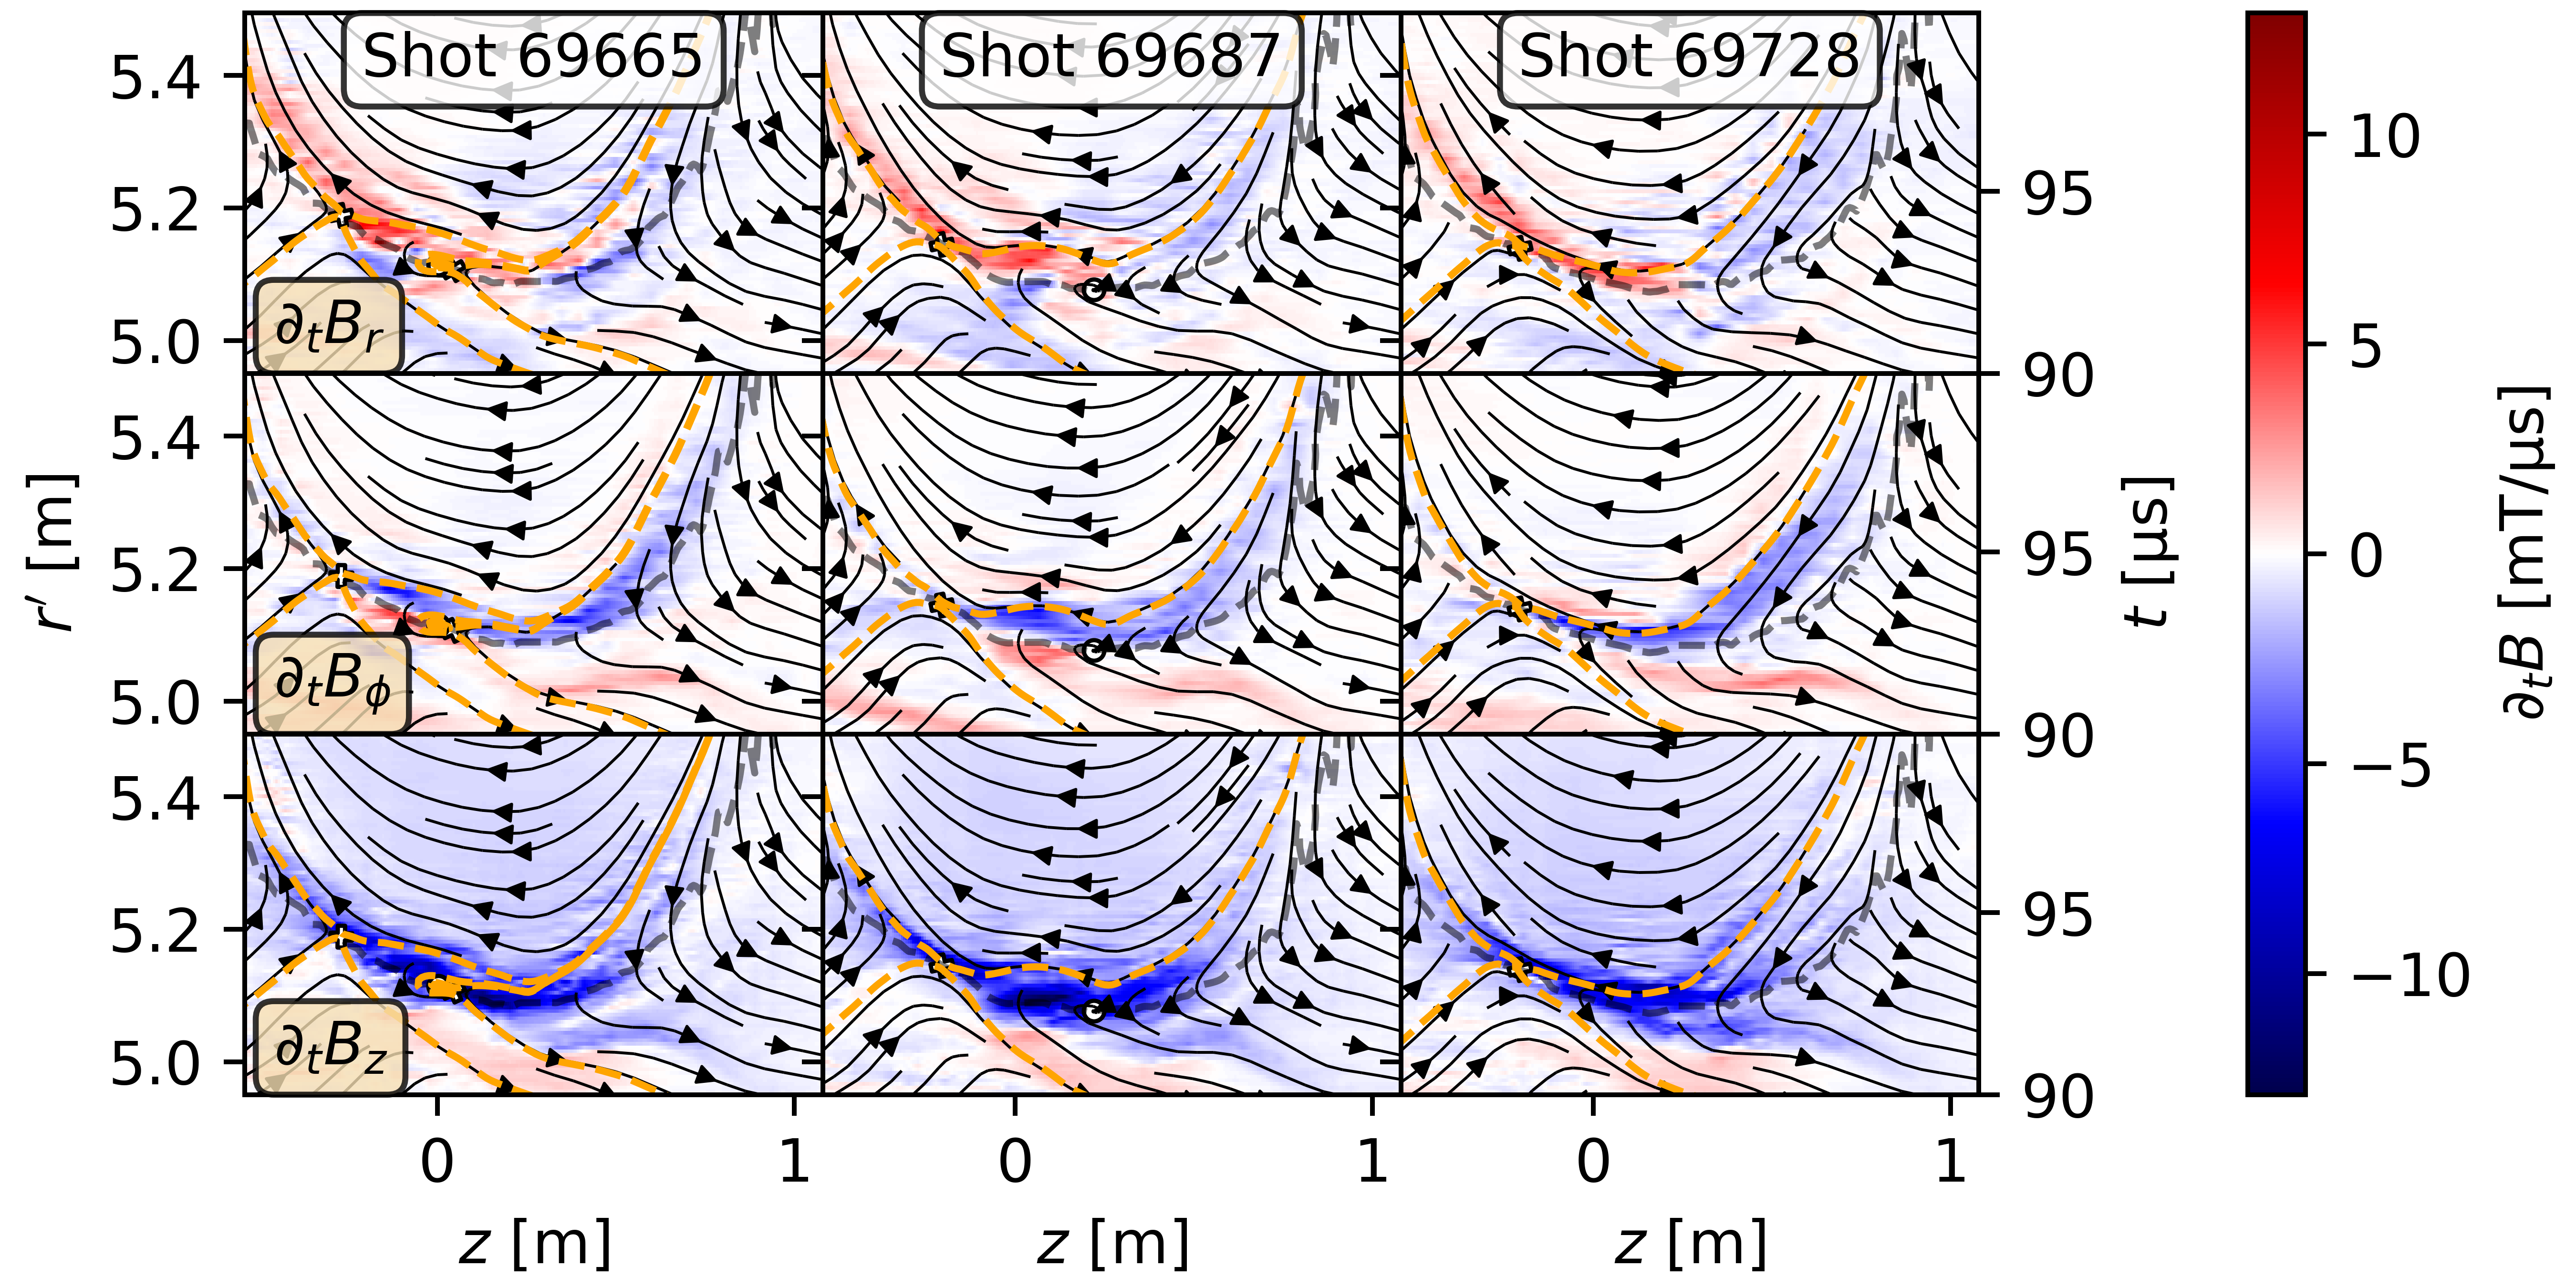
\includegraphics[width=\textwidth]{chapter_pa_probe/figures/example_lightsaber_measurements.png}
    \caption[Lightsaber Probe Measurements]{This figure shows three different shots (columns) and their respective B-dot measurements in various directions (rows). Most shots are like that of shot 69728 where there is a single x-point for many of our configurations but sometimes during a shot, plasmoids can form like those in shots 69664 and 69687. These plasmoids can form either to the left or right of the main reconnecting x-point and can change the outflow dynamics of the reconnecting current layer.}
    \label{fig:pa_lightsaber_plots}
\end{figure}

We have to use many shots to build up a full IV-characteristic for the PA probe and different machine setups/parameters lead to different amounts of reproducibility. In the plasmas we are studying while looking for pressure anisotropy, we find the dominant source of irreproducibility are plasmoids that form near the x-point and are ejected into the outflow (shots 69665 and 69687 in figure \ref{fig:pa_lightsaber_plots}). It is relatively easy to pick out shots that vary drastically by eye from these lightsaber probe measurements (see \ref{sss:diagnostics_overview} for the probe description).

We can also remove bad shots by comparing all shots where the PA probe was at the same bias. If a shot gives signals for all the tips that are very different than the other shots we remove the outlier shot.

% \subsubsection{Averaging of core data}
% \label{ss2:pa_averaging_relay}

To average the data we start by finding clusters of shots where the bias voltage, $V_{\text{bias}}$, is within some tolerance of each other (usually $~5$ V). Then we calculate $I_\text{probe}$ and $V_\text{probe}$ for each shot. For each cluster of shots of size $N$ there will be $n$ shots with the core signals un-swapped and $N - n$ shots with the signals swapped. Then our averaged data can be written as
\begin{align*}
  I_\text{probe}^\text{avg} &= \frac{1}{2} \left( \frac{1}{n} \sum_{i \in n} I_\text{probe}^i + \frac{1}{N - n} \sum_{i \in N - n} I_\text{probe}^i \right) \\
  &= \frac{1}{2 n (N - n)} \sum_{i \in n} \sum_{j \in N - n} \left( I_\text{probe}^i + I_\text{probe}^j \right) \\
  V_\text{probe}^\text{avg} &= \frac{1}{2 n (N - n)} \sum_{i \in n} \sum_{j \in N - n} \left( V_\text{probe}^i + V_\text{probe}^j \right).
\end{align*}
Here we have normalized our averaging terms by the number of shots in each cluster.

% \subsection{Fitting shell}

The shells act very much like a normal Langmuir probe in that they collect isotropically and thus their analysis is relatively simple. We use all the data from all of the shots which creates a large distribution of points on the IV-characteristic and additionally combine all the tips together while fitting such that we measure $n_e^\text{shell}$, $T_e^\text{shell}$, and $V_\text{plasma}$. Example fits from the routine can be seen in figure \ref{fig:pa_example_shell_fits}.

\begin{figure}
    \centering
    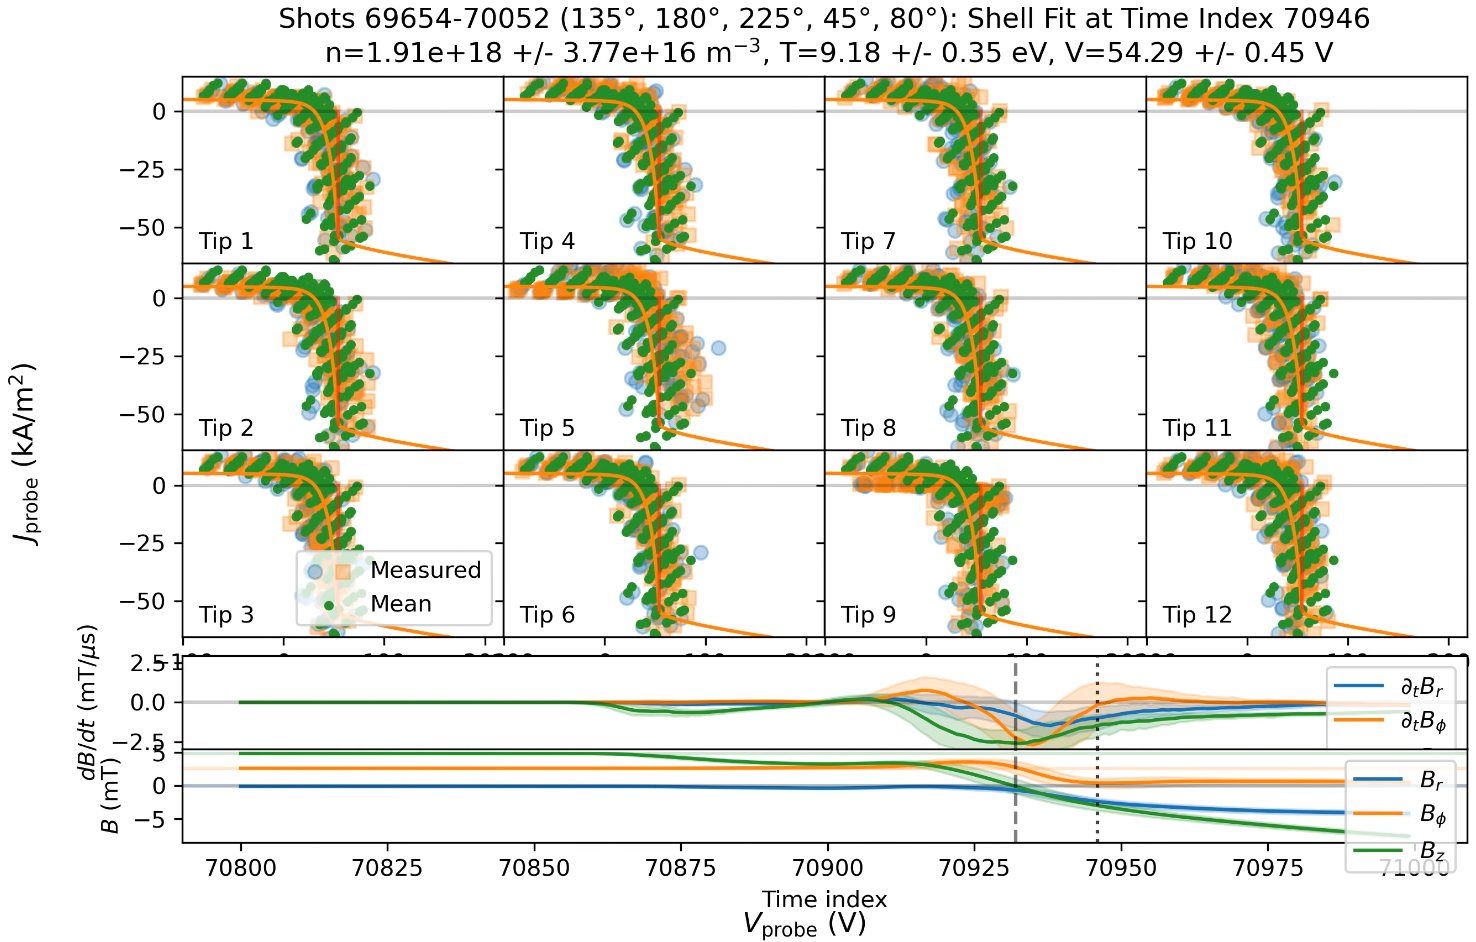
\includegraphics[width=\textwidth]{chapter_pa_probe/figures/shell_fit_screen_grab.png}
    \caption{Example fits for the shell data at a single time after combining many shots and clocking angles (shot numbers and angles can be seen in the figure title). The bottom two panels show the magnetic field evolution with error bars being the standard deviation between all the PA probe magnetic field measurements. The dashed black line is the location where $B_z = 0$ and the dotted black line is the time for the shown shell IV-characteristics. The twelve panels each show the individual tip measurements in pale blue or orange for swapped vs. un-swapped core while the mean value of all the tips for a given shot is in green. The solid orange lines are the fit BRL characteristics with the red line being the plasma voltage.}
    \label{fig:pa_example_shell_fits}
\end{figure}

% \subsection{Fitting core}

In fitting the core IV curves we fit each tip individually as the full IV-characteristic model suffers from some issues as described in \ref{sss:pa_individual_tip_fitting}.
We fit each tip using a similar routine as done for the core and multi-tip Langmuir probe in that we use Orthogonal Distance Regression (ODR) along with the exponential plasma model.
% \subsubsection{Individual fitting method}

% \paragraph{ODR errors}

ODR requires a way to model the error on the measured parameters (i.e. the bias voltage and the various digitizer measurements) that propagates to the model to fit. For the multi-tip Langmuir probe we were able to fully model the errors we expect to appear in $V_\text{probe}$ and $I_\text{probe}$ since both of those derived measurements depended solely on the measurements during a single shot. Thus if there is an error on $v_{ds}$ of $\sigma_{ds}$, this would lead to an error of $\sigma_{V,\text{probe}} = V_\text{probe}(v_{ds} + \sigma_{ds}) - V_\text{probe}(v_{ds})$ (a similar analysis can be done for $I_\text{probe}$ where this example used the variables as seen in equations \ref{eq:multitip_V_p} and \ref{eq:multitip_I_p}). Then all errors on the bias voltage and the probe signals can be incorporated into the fitting routine.

Since we will be using data averaged over many shots, there are other sources of error to account for like variable time delays and irreproducable plasma parameters. We find that a good alternative to a full error model is by setting the error of the probe current and voltage to
\begin{align*}
    \sigma_{I,pc} &= \tilde{I}_{pc} - I_{pc} \\
    \sigma_{V,pc} &= \tilde{V}_{pc} - V_{pc}
\end{align*}
where the tilde represent the the measured signal with some error (like what $v_{ds}$ was in the last example). $\sigma_{I,pc}$ and $\sigma_{V,pc}$ are set such that $\sigma_{V,pc} = R_s \sigma_{I,pc}$. The magnitude of this error does not matter for fitting as ODR will try to minimize the error in the same way independent of a scaling factor on both errors. By choosing an error like this, the fitting routing will use ellipses oriented along the current and voltage axis in the IV-characteristic fitting (the example consisted of errors acting as skewed ellipses that were aligned with $J \approx V / R_s$).

% \paragraph{Exponential fitting method}

% \paragraph{Constant Plasma Potential}

\section{Results}

% \subsection{Drive cylinder}

As described in \cite{Gradney_Egedal_Barnhill_Flores-García_Greess_Kuchta_Olson_Wallace_Yu_Forest_2023}, we have installed a drive cylinder that acts like many individual coils in parallel. This decreases the inductance of our system, driving the reconnection layer with much larger loop voltage leading to a higher Lundquist number. The drive cylinder also generates a long uniform current sheet which is useful for studying basic physics of reconnection without some of the edge effects that come from discrete coils.

To identify configurations with pressure anisotropy, we searched the experimental parameter space for the existence of a third current jet in the $\partial_t B_z$ data. As we were only using the flux arrays for this search, the resolution of the coils in the $z$ direction is 12 cm. This was too large of a distance to identify any jets in our system and thus were unable to identify shots with magnetic field features matching anisotropy.

Since the drive cylinder increases the speed of the layer, this leads to fewer data points in the outflow reducing the signal-to-noise ratio of our data and requiring higher timing accuracy.

For future studies, B-dot probes with high $z$ resolution like the lightsaber probe, may be able to identify when to use the PA probe but we have thus far been unable to identify anisotropy with the drive cylinder.

% \subsection{3 coil}

We were able to measure pressure anisotropy in our three coil system that successfully reproduced the expected measurements from simulation. Figure \ref{fig:pa_wetherton_vpic} shows a cut through a particle in cell simulation that reproduced features similar to those seen in spacecraft (see \cite{Wetherton_Egedal_Le_Daughton_2022}). These traces show a number of features. The top plot shows $J_\phi$ which in our system is proportional to $\partial_t B_z$. Here, there are three distinct current jets, two that follow the separatrices and a third the bisects the outflow. Taking a trace through the outflow (brown and green line) the magnetic field drops in the outflow but does not reach zeros while the temperature anisotropy has a double peaked feature. The jet appears in a region of high anisotropy where the marginal firehose condition, $F$, approaches $0.5$.

\begin{figure}
    \centering
    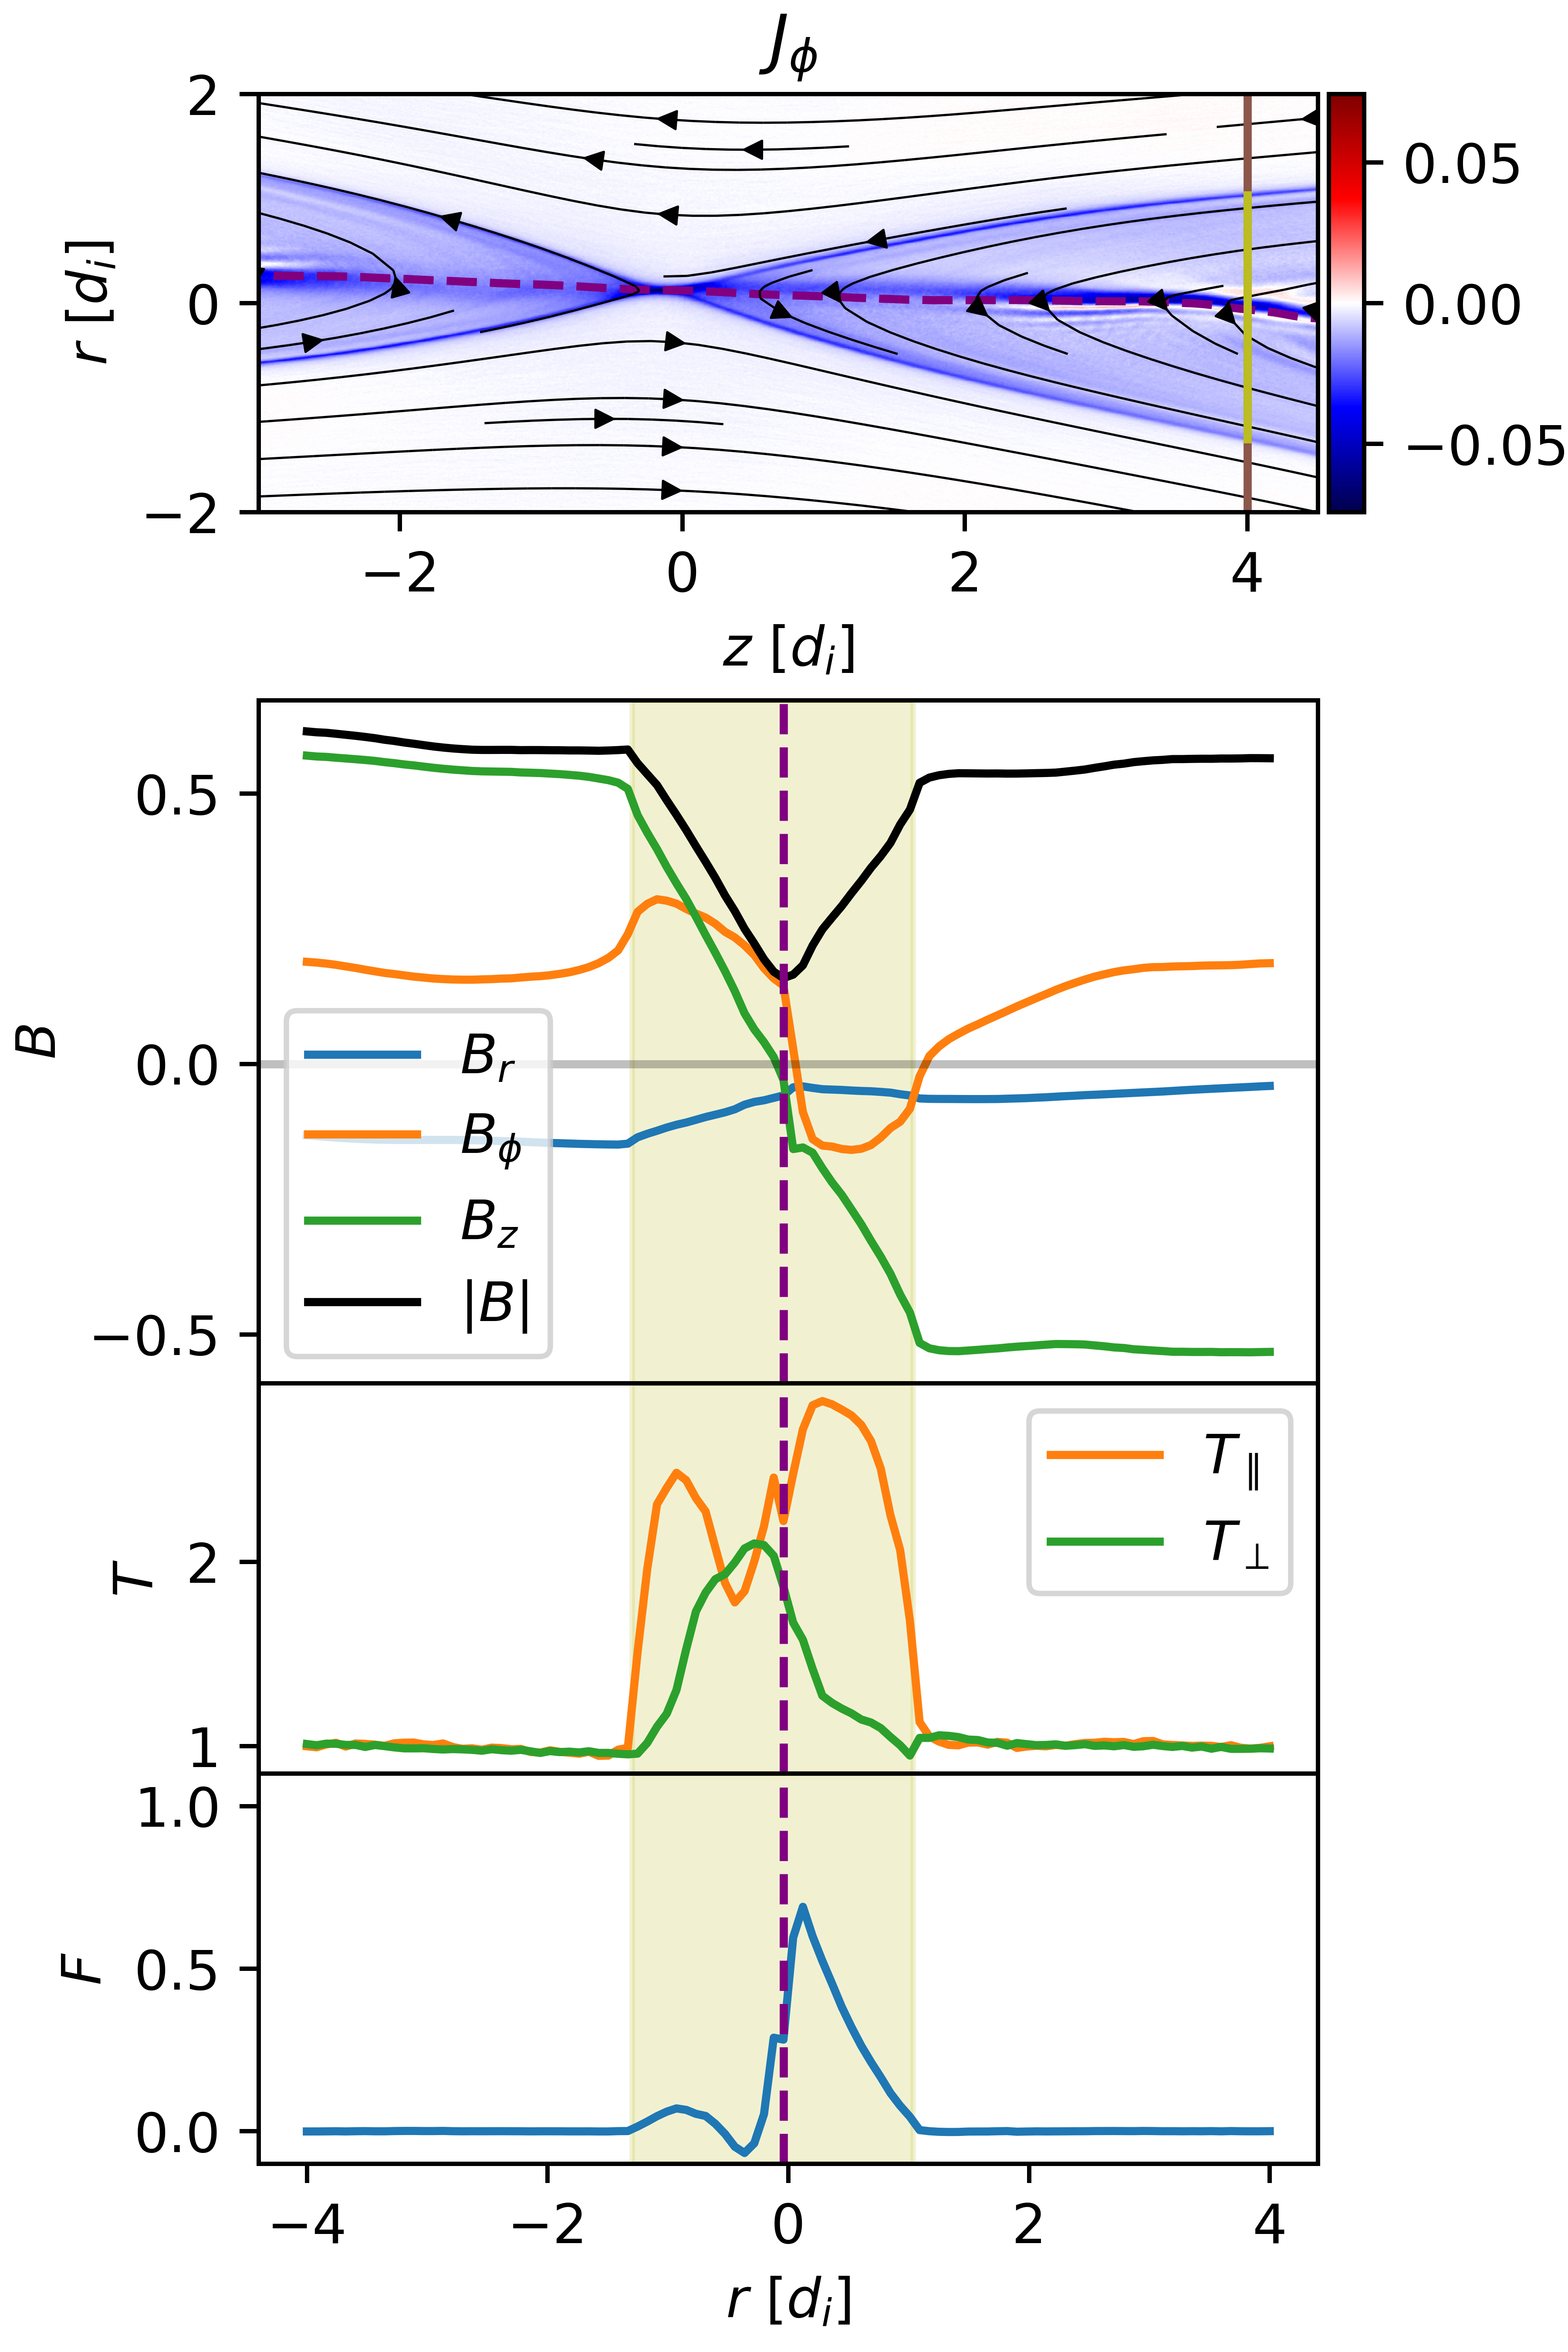
\includegraphics{chapter_pa_probe/figures/wetherton_vpic_cut.png}
    \caption{Data reproduced from \cite{Wetherton_Egedal_Le_Daughton_2022}. The top plot shows the out of plane current with a clear three jet structure in the outflow. When taking a trace through the outflow, shown by the brown and green line, the magnetic field, anisotropy, and firehose condition are plotted. The field drops to a non-zero value and at the jet the pressure anisotropy is large with a firehose condition of approximately 0.5.}
    \label{fig:pa_wetherton_vpic}
\end{figure}

From our magnetic field data, we can see that there are three jets in the outflow which are reproducible (see figure \ref{fig:pa_lightsaber_with_jet}). This implies that the cause of this third jet should be measurable and from prior work may be due to pressure anisotropy.

\begin{figure}
    \centering
    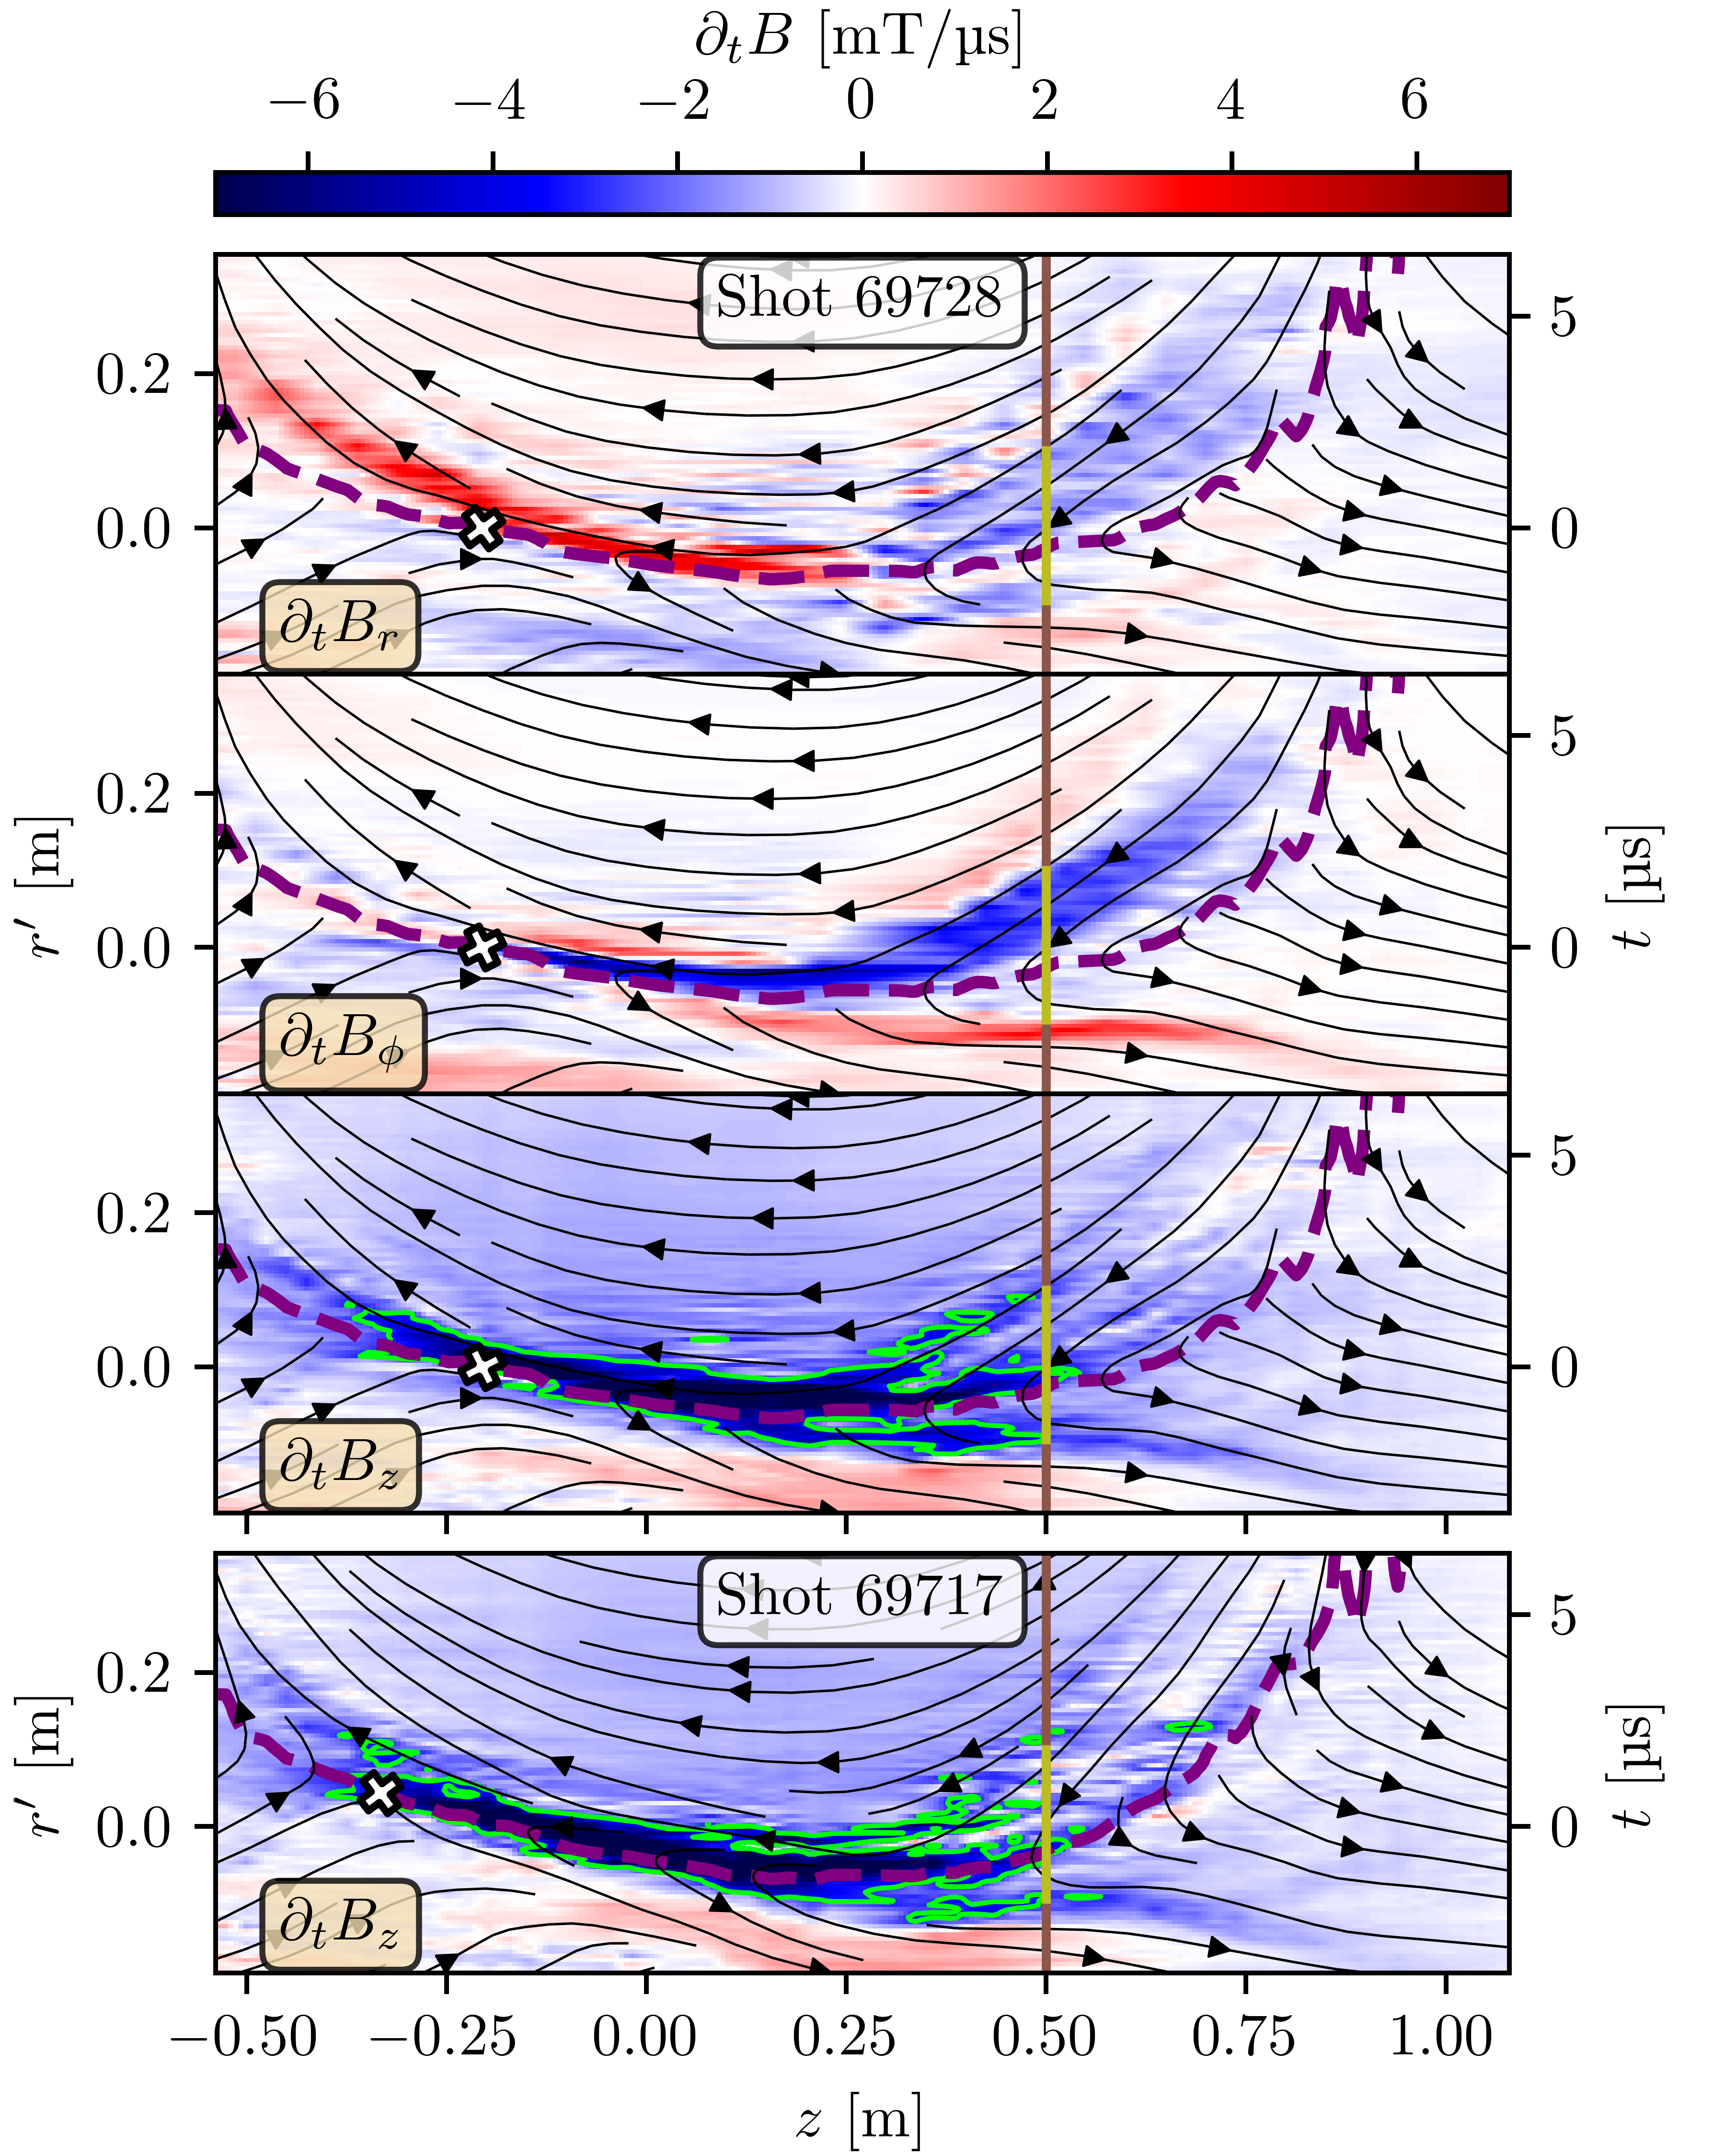
\includegraphics{chapter_pa_probe/figures/example_lightsaber_measurements_69728_69717.png}
    \caption{Measurements of the lightsaber probe for two separate shots. The black streamlines are the direction of the field and the x's are the location of the x-point calculated using the winding number. The green contour in the $\partial_t B_z$ data highlights the three jets. The right axis is the time coordinate centered at the x-point while the left axis is an approximate position derived from the ``jogging'' method \cite{Olson_2020}. Both shots show similar outflow features even though the x-point is moved to the left in shot 69717 compared to shot 69728.}
    \label{fig:pa_lightsaber_with_jet}
\end{figure}

\begin{figure}
    \centering
    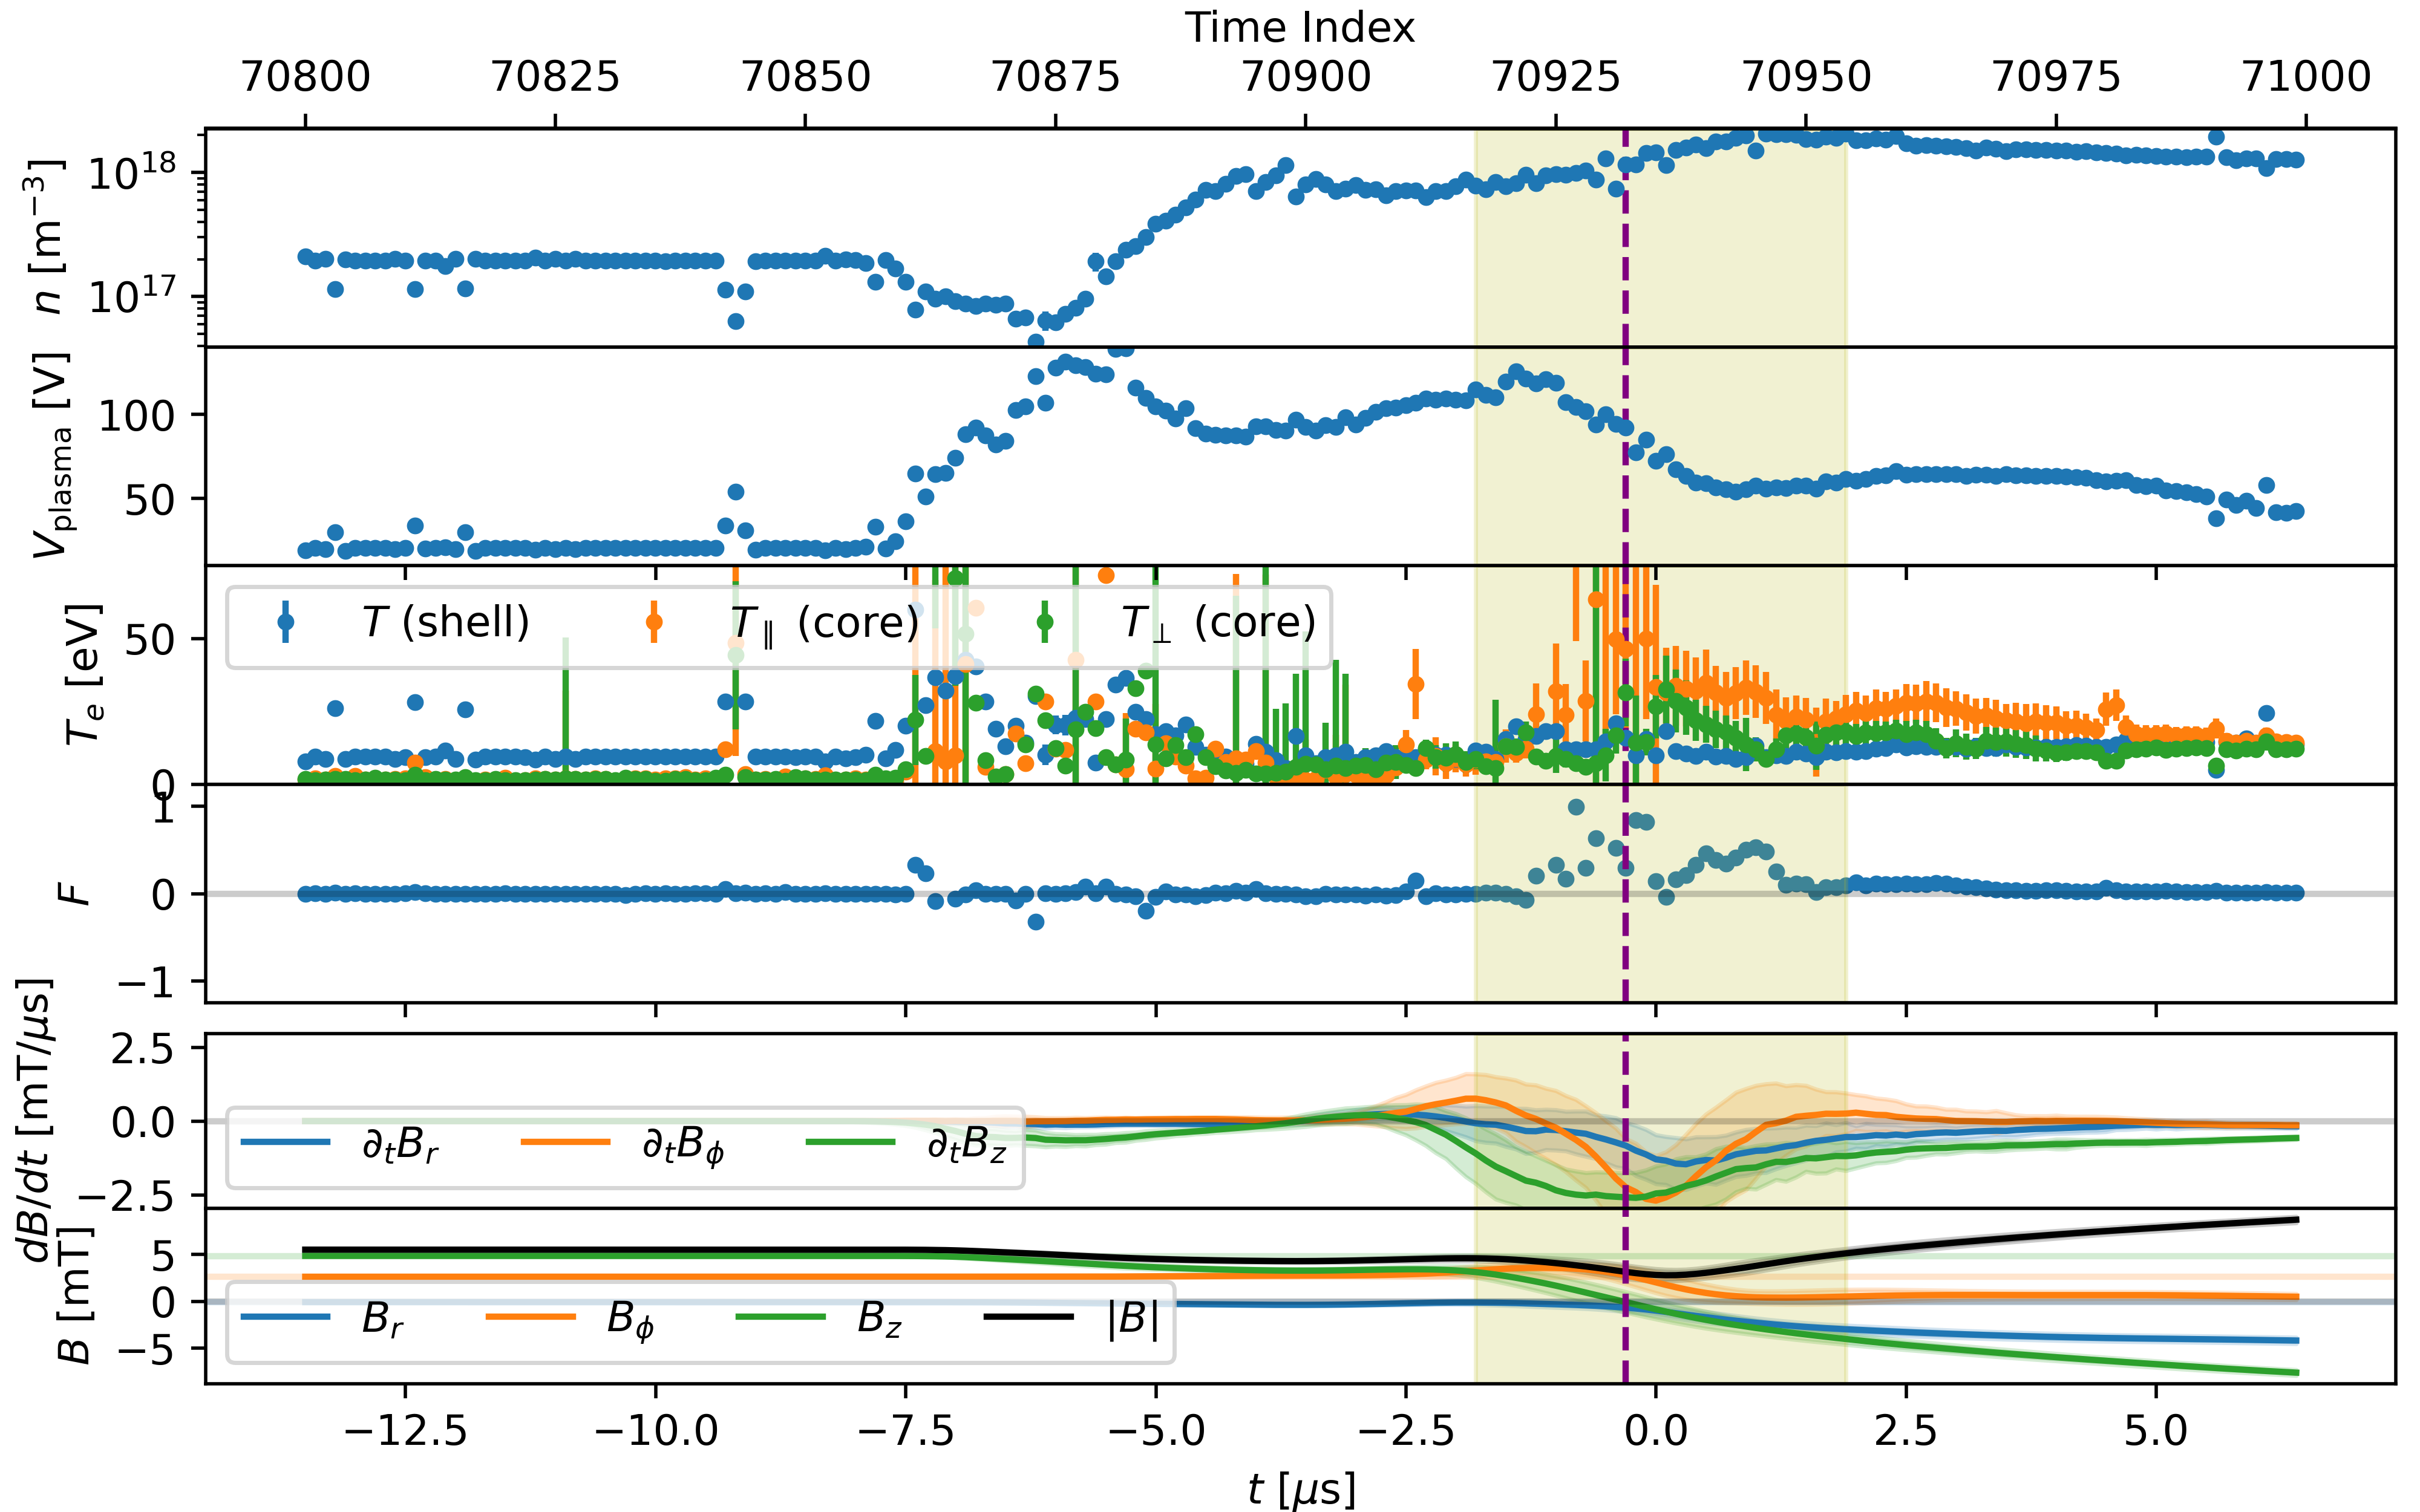
\includegraphics[width=\textwidth]{chapter_pa_probe/figures/fits_69654-70052_clock_45_80_135_180_225.png}
    \caption{Measurements from the pressure anisotropy probe during a shot with high guide field. Pressure anisotropy exists in and around the outflow (highlighted by the green box) and while in the outflow the firehose condition approaches 0.5 as expected from simulation and spacecraft. The dip in firehose condition is also expected as can be seen in figure \ref{fig:pa_wetherton_vpic}.}
    \label{fig:pa_high_field_results}
\end{figure}

B-dot measurements are not enough to confirm nor deny pressure anisotropy so we employ the PA probe. Results of those measurements can be seen in figure \ref{fig:pa_high_field_results}. The PA probe sees many of the same features as seen in \ref{fig:pa_wetherton_vpic} with an increase in pressure anisotropy in the outflow and a similar double peaked structure in the marginal firehose condition. The magnetic field magnitude additionally shows a similar dip in strength while staying greater than zero.

The anisotropy we measure may be due to some tips always measuring a higher temperature and the moving field causing the anisotropy to show only in the outflow. To check for this we've applied the aforementioned tri-Maxwellian analysis to the measurements and found that in the outflow the highest temperature is almost always more parallel to the field than the cooler two temperatures as can be seen in figure \ref{fig:pa_hodogram}.

\begin{figure}
    \centering
    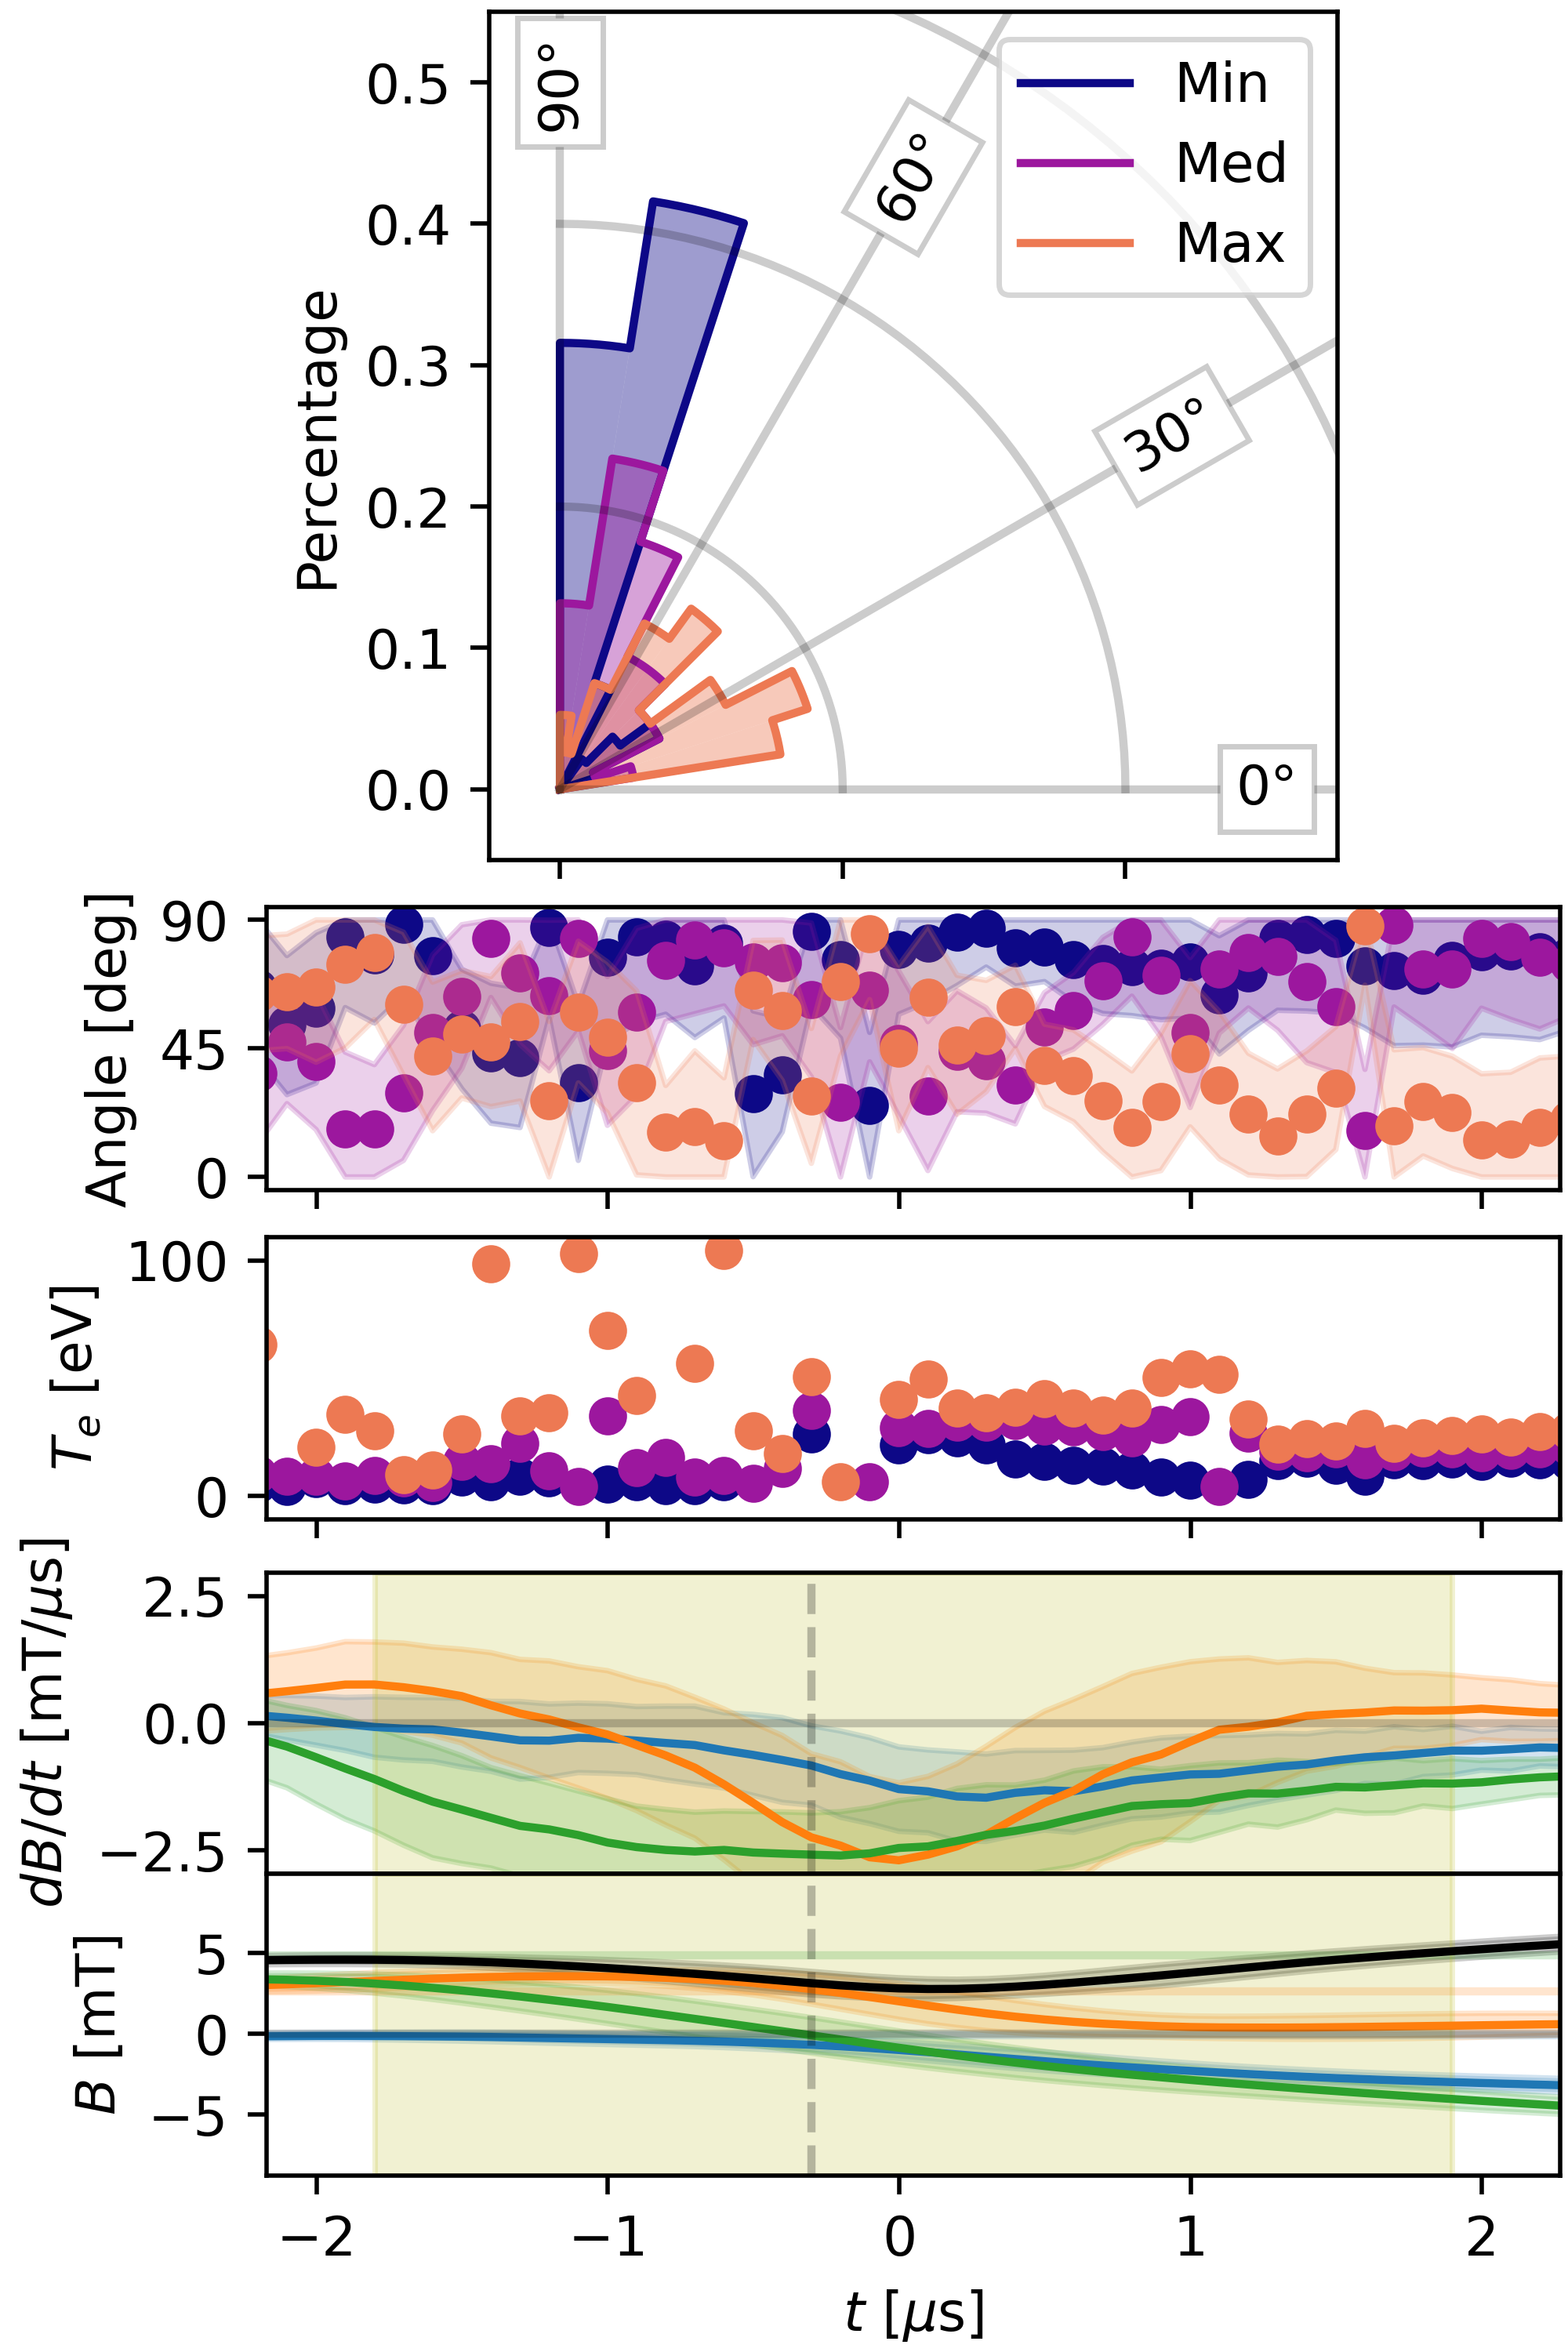
\includegraphics{chapter_pa_probe/figures/b_proj_69654-70052_clock_45_80_135_180_225.png}
    \caption{This plot shows how the tri-Maxwellian analysis performs in the outflow of reconnection. The top plot shows a histogram of the minimum (`min'), median (`med'), and maximum (`max') temperatures relative to the magnetic field. It can be seen that the hottest temperature is most often relatively parallel to the magnetic field. The second panel shows the angles of these temperatures with respect to the field once again showing that the higher temperatures are more parallel especially later on in the outflow. The third panel shows the temperatures from the tri-Maxwellian analysis. The histogram is only calculated in the outflow.}
    \label{fig:pa_hodogram}
\end{figure}

When we reduce the guide field we see the jet disappear and a reversal in the pressure anisotropy. We expect that this is due to isotropization of the distribution function at the x-point (due to lack of magnetic moment conservation). When the flux tubes leave the x-point they undergo a process that is the opposite of what occurred during on inflow. The flux tubes compress in the perpendicular direction and extend in the parallel leading to a perpendicular temperature that is higher than the parallel temperature. This can be seen in figure \ref{fig:pa_no_field_results}.

\begin{figure}
    \centering
    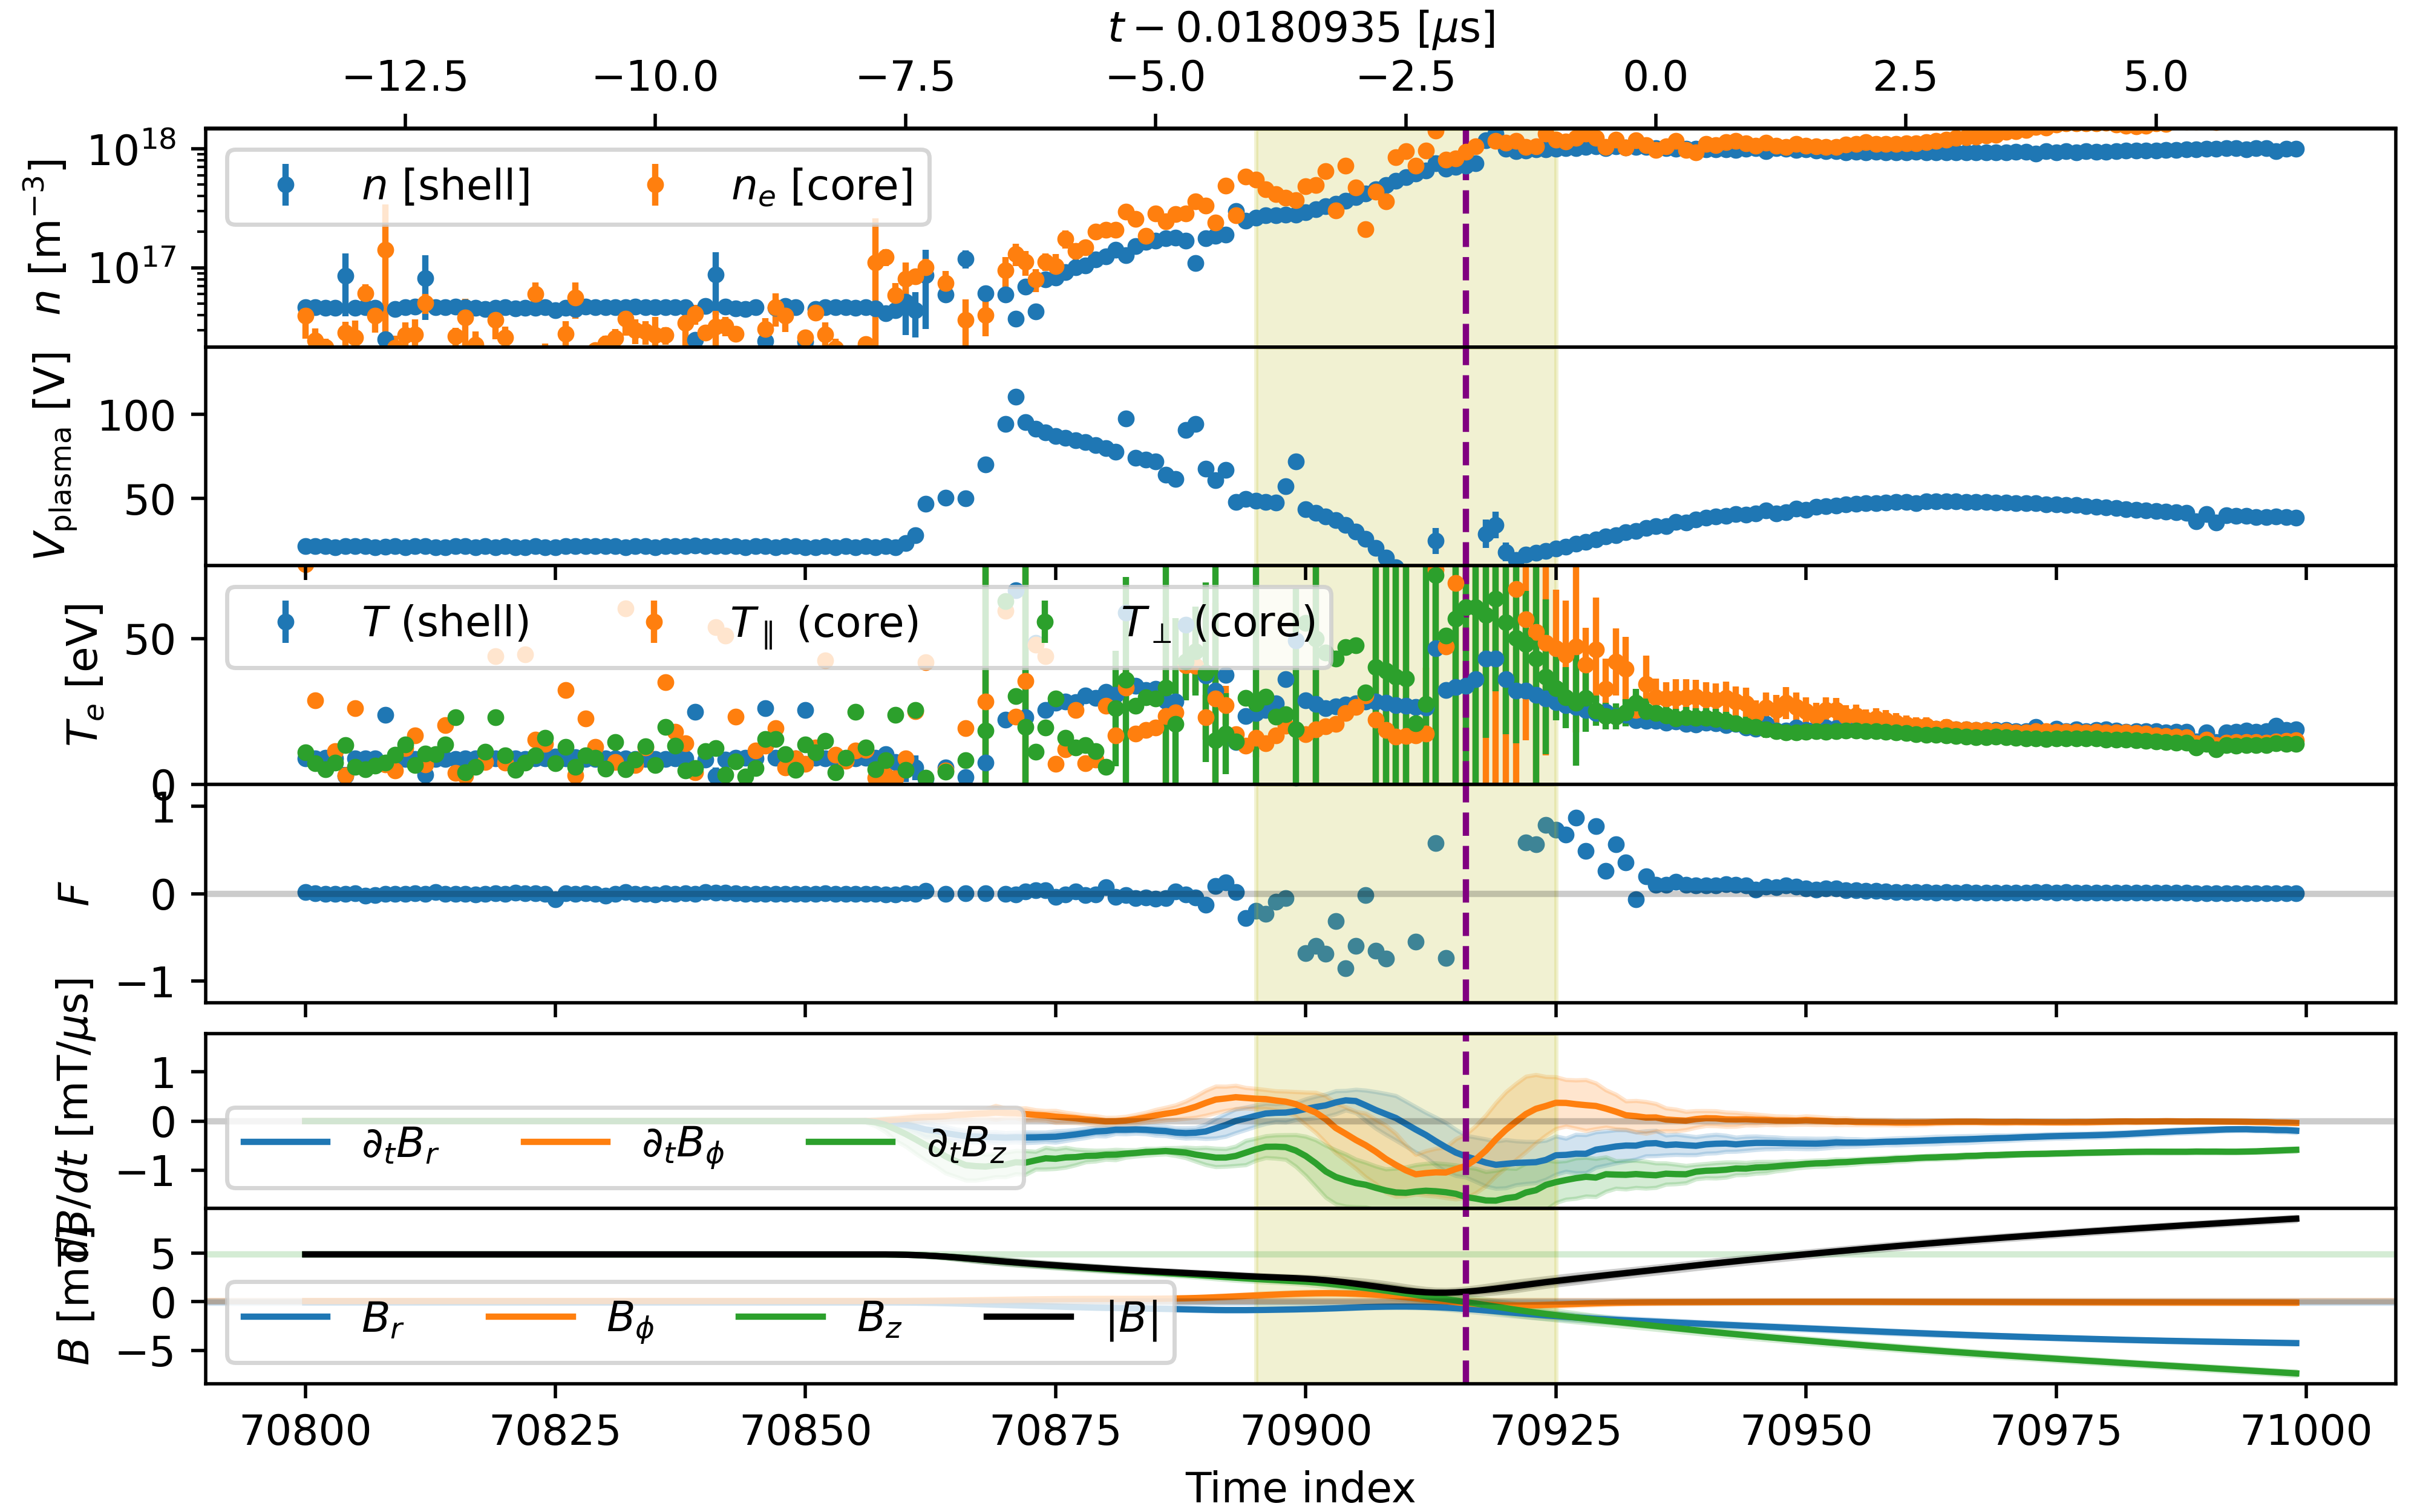
\includegraphics[width=\textwidth]{chapter_pa_probe/figures/fits_70267-70410_clock_45_90.png}
    \caption{The same figure setup as \ref{fig:pa_high_field_results} except the plasma had no guide field, $B_\phi$. The outflow has $T_\perp > T_\parallel$ which is expected due to isotropization at the x-point.}
    \label{fig:pa_no_field_results}
\end{figure}
